\documentclass[draftthesis,fancy,edeposit]{uiuc_thesis_template}

\usepackage{epigraph,hyperref}
\usepackage[backend=bibtex,style=numeric-comp]{biblatex}
\usepackage{graphicx}
\usepackage{multirow}
\usepackage{amsmath}
\usepackage{seqsplit}
\usepackage{bm}
\usepackage{rotating}

%\bibliography{Bibliography/intro}
\bibliography{Bibliography/ML}
\bibliography{Bibliography/calo_ML}
\bibliography{Bibliography/SUSY}

\begin{document}

\newcommand{\MET}{$E_{T,miss}$}
\newcommand{\mll}{$m_{\ell\ell}$}
\newcommand{\mindphijm}{$\Delta\phi(E_{T,miss},jet_{1,2})_{min}$}
\newcommand{\chpi}{$\pi_{\pm}$}
\newcommand{\pizero}{$\pi_0$}
\newcommand{\pt}{$p_T$}
\title{A Search for Supersymmetry with the ATLAS Detector, and the Use of Machine Learning Techniques for Object Classification in High Energy Physics}
\author{Matt Zhang}
\department{Physics}
\schools{B.S. University of Texas at Austin, 2013}
\phdthesis
\advisor{Ben Hooberman}
\degreeyear{2021}
\committee{Associate Professor Ben Hooberman\\
Professor Mark Neubaeur\\
Associate Professor Jessie Shelton\\
Professor Lance Cooper}
\maketitle

\frontmatter

\begin{abstract}
We conduct a search for supersymmetry using data from the ATLAS detector at CERN, in a region with 2 leptons, 2 jets, and large \MET. We also demonstrate the development of various machine learning techniques to enhance similar physics searches in the future, including the use of neural nets on calorimeter data for particle-type classification, particle energy regression, and shower generation.
\end{abstract}

\chapter*{Acknowledgments}

This thesis is for my friends, who almost managed to keep me sane after all these years. I'd also like to thank my advisor Ben Hooberman, for helping me grow into a confident and competent researcher. My gratitude also goes out to my lab mates, and to all the students, professors, and staff of UIUC for creating such a nurturing learning environment. And of course, I'd like to thank the community at CERN for supporting the international particle physics community and allowing this type of research to flourish. %[text]
\chapter*{An Introduction}

If you are reading this thesis, then I have either applied for or have  already received my PhD in Physics from UIUC. If it's the former, thanks for coming to my thesis defense.

I'm going to try to convince you that I know some things about particle physics, and that I've done some things worthy of a doctorate. Hopefully I'll even teach you something new along the way.

Here's a short summary of my thesis, in case you're skimming it over ten minutes before my defense:

\begin{itemize}

    \item Like many particle physicists over the years, I've spent my graduate career searching for evidence of extensions to the Standard Model. My thesis begins by describing the Standard Model and the supersymmetric (SUSY) models which we were hoping to find evidence for\footnote{Spoiler: we found no such evidence.}.
    
    \item After this, I briefly describe the relevant components of the detector with which our precious PhD-sustaining data was collected, and walk through the basic steps and terminology of a particle physics search.
    
    \item Next up is a description of the SUSY search which forms the bulk of my thesis work. This is the section which proves that I am actually a physicist as opposed to a computer scientist. I describe the details of our search, and describe my contributions to the project.

    \item My particular specialty is in machine learning, which in recent years has come to dominate the field of artificial intelligence to such a degree that the terms might as well be interchangeable. I describe how machine learning works, including the general classes of techniques which I used in my various studies.
    
    \item After that I go through details of two machine learning studies which I led.
    
    \begin{itemize}
    
        \item The first study was on the identification and generation of particle showers in calorimeters. This means that we wrote an algorithm which is able to look at a calorimeter shower after a collision event and both determine what type of particle produced the shower and how much energy the particle had. We could also artificially generate showers for different particles at various energies, a technique which may allow us to circumvent computationally-intensive Monte Carlo (MC) simulations in the future. My main focus was the particle classification section, though I contributed to all parts of the project.

        \item The second study was on the identification of heavy-flavor-decay leptons, which form the largest background in a number of searches. This study used recurrent neural nets (RNN's) to perform lepton classification based on track information.

    \end{itemize}

    \item Following this I describe some detector upgrade related work and other small projects that I have done, including:
    
    \begin{itemize}
        \item work on the Fast TracKer upgrade (FTk)
        \item pixel detector assembly and beam testing work which I did during a one-year residency at Argonne National Lab
        \item improvements to vertex reconstruction algorithms
    \end{itemize}

    \item And of course, no thesis is complete without a conclusion, in which I'll basically tell you all of this information again, except now you'll understand what I'm talking about. I'll also describe methods of applying the machine learning tools I have built to future physics searches.

\end{itemize}

Thanks for reading my thesis. Let's begin.

\tableofcontents
\listoftables
\listoffigures
\chapter*{List of Abbreviations and Definitions}

\begin{symbollist*}
\item[$\eta$] Also known as pseudorapidity. $\eta=-ln(tan(\theta/2))$. $\eta$ is typically used rather than $\theta$ because differences in pseudorapidity are relativistically invariant to boosts along the beam axis.
\item[$\theta$] Angle measured from the beam axis.
\item[ATLAS] A Toroidal LHC ApparatuS. A detector at the LHC.
\item[background] Expected events from known components of a theory. For example, Standard Model events would be the background in a SUSY search.
\item[baryon] A composite particle made of three quarks. Protons and neutrons are examples of baryons.
\item[beam] A stream consisting of billions of particles. Two beams are circulated in opposite directions in a circular collider and made to cross at a collision point. Beams consist of many separated bunches.
\item[beam axis] Line formed by the path of a beam through the detector. The two colliding beams in a detector are actually at a very small angle to each other when they cross, but the average is taken as the beam axis.
\item[boson] A particle with integer spin. Examples include photons, W and Z bosons, and mesons.
\item[bunch] A tight cluster of particles in a beam. Each bunch in the LHC is typically several centimeters long and a few micrometers wide.
\item[bunch crossing] The collision of two bunches in a detector, resulting in a single event.
\item[CERN] Conseil Européen pour la Recherche Nucléaire. A multinational high-energy physics experiment operating on the French-Swiss border.
\item[CM] Center of mass. This is the inertial frame in which a system's total momentum vector is zero.
\item[CM energy] Center of mass energy. This is the total amount of energy present in a system's rest frame, including mass energy. Can also be seen as the magnitude of the system's energy-mass four-vector.
\item[cross section] A measure of probability that a specific particle interaction or decay will take place, analogous to the actual cross section of a hard body in a two-body collision.
\item[data] Events reconstructed from actual collisions, as opposed to MC events.
\item[decay] The spontaneous transformation of one particle into two or more particles.
\item[$E_T$] Transverse energy. Defined as $E_T = sqrt(m^2 + p_T^2)$.
\item[event] Detector recording of a single bunch-bunch collision.
\item[excess] When the number of measured events are greater than the number of expected events from background. Excesses are measured in sigmas, or the number of standard deviations above background.
\item[exclusion] A model is excluded if a search finds that the model is less likely to have produced measured data than the Standard Model by some statistical likelihood.
\item[fermion] A particle with half-integer spin (e.g. $1\frac{1}{2}$). These include all leptons and baryons.
\item[FTk] Fast TracKer. A hardware-based track reconstructor which is part of the ATLAS trigger system.
\item[FPGA] Field programmable gate array. This is a single-purpose chip without an operating system. It's programmed directly at the electronic gate level.
\item[hadron] A composite particle made of two or more quarks. Includes all mesons and baryons.
\item[hard scatter] The primary interaction in a proton-proton bunch crossing, containing objects of sufficient energy to be considered interesting. This is opposed to pileup interactions.
\item[HEP] High energy physics. Also known as particle physics.
\item[jet] A spray of particles produced by the decay chain of a quark or gluon as it travels through a detector.
\item[lepton] Electrons, muons, taus, and their associated neutrinos and antiparticles.
\item[LHC] Large Hadron Collider. A circular proton-proton collider operating at CERN.
\item[LSP] Lightest SUSY particle. The lightest particle in a SUSY model.
\item[meson] A composite particle made of two quarks.
\item[MC] Monte Carlo. A class of algorithms based on random sampling. In high-energy physics, MC events (as opposed to data events) are simulated via MC algorithms, rather than gathered from actual collisions.
\item[\MET] Missing energy. This is an $E_T$ vector which would have to be added to an event for it to have a total $E_T$ of zero. \MET is an indication of a non-interacting or mismeasured object.
\item[model] An HEP model describes which particles exist in nature and how they interact. e.g. the Standard Model.
\item[pileup] The number of proton collisions per bunch crossing. Most of these collisions are not good, and produce soft objects that mainly serve to obscure the interesting hard scatter event.
\item[\pt] Transverse momentum. The radial component of an object's momentum, as opposed to the components in the beam axis or azimuthal directions.
\item[RNN] Recurrent neural net. A neural architecture described in Section~\ref{sec:advanced_architectures}.
\item[search] An attempt to find evidence that collision data is better described by an alternative model than by the Standard Model. e.g. SUSY search.
\item[SM] Standard Model. This model describes how the electromagnetic, weak, and strong forces interact with all known elementary particles, and is described in Chapter~\ref{chap:SM_SUSY}.
\item[SUSY] Supersymmetry. A class of models described in Chapter~\ref{chap:SM_SUSY}.
\item[trigger] A hardware or software-based set of criteria which must be passed in order for an event to be saved. E.g. the presence of at least one particle in the event with \pt $>$ 10 GeV.

\end{symbollist*} %[text]

\mainmatter

\part{A Brief Introduction to Particle Physics}
\chapter{The History of Understanding the History of Everything}

In the beginning people knew nothing. What is the universe made of? Can you turn a rock into gold? What happens if you get smaller and smaller - is there a whole different world down there? These were just a small subset of questions our early ancestors would never know the answer to, since they all died out before the development of particle physics in the $20^{th}$ century. But let's entertain ourselves by examining a few of the early mental models they had, and how the persistent desire to improve these models led to the development of modern physics.

It's somewhat strange at first glance that many ancient cultures had roughly the same classical elements, but upon examination of the things commonly found in nature, we can understand where these groupings came from. Most early building materials, food, and organic compounds came out of and into the earth. These things seemed to cycle endlessly and turn easily into each other, so the element of earth or clay logically served as a catch-all building block for all such materials. Chinese philosophy further divided wood and metal into their own categories separate from earth. Next came fire and water, distinct enough from earth to warrant separate categories of their own. Together, earth, water, and fire also roughly corresponded to the common states of matter (solid, liquid, gas/plasma), so it's understandable that these mental clusterings became common in many early philosophies. The elements of air and aether were somewhat unique to Greek thought however, and were probably later transported into India and folded into the classic Buddhist elements.

In all then, we had air, water, earth, fire, and aether in Greek philosophy, corresponding to the five Platonic solids~\cite{Plato}, and according to Empedocles~\cite{Empedocles}, bound together by love and strife. In Indian philosophy we had air, water, and earth, corresponding to different categories of food~\cite{Chandogya}. This evolved with Greek influence into the five elements of early Buddhism and Hinduism, each with their own associations~\cite{friesian}. In Chinese philosophy we had metal, wood, earth, water, and fire~\cite{Tao}. When combined with air and aether, the system was further expanded to form associations with the sun, moon, and five visible planets~\cite{friesian}.

And so we see how throughout the ancient world, a complex series of inter-related, "common-sense", and entirely wrong memetic systems came to dominate early philosophy. Based on pattern recognition and concept association rather than experimental evidence, these unscientific models guided intellectual pursuits for many centuries. There is a tendency among physicists to trace the beginnings of atomic theory back to the Greek philosopher Democritus, but without the use of scientific experimentation guided by mathematical modelling, his philosophy had no more value than these other ancient systems, aside from the irrelevant distinction of ultimately being correct.

It was not until the chemical revolution of the $16^{th}$ to $18^{th}$ centuries that we had (from a modern standpoint) acceptable proof of the existence of tiny building blocks of nature. Careful experiments carried out during this time allowed scientists to measure the masses of compounds before and after chemical reactions. Various elements were separated for the first time, and the role of oxygen in combustion was discovered. In his book "New System of Chemical Philosophy", John Dalton compiled relative masses of known elements, providing evidence for the existence of atoms~\cite{new_system_chemical}. Dalton was also able to use his system to calculate the composition of elemental gasses in the atmosphere. Einstein's later work on Brownian motion in 1905 provided further evidence that atoms and molecules exist.

Feynman argued in his Lectures on Physics~\cite{feynman1965flp} that the existence of atoms was the most important knowledge in modern science, from which most of the rest could be derived. However, demonstrating the existence of atoms was not the end of the line for tiny physics. The Rutherford gold foil experiment~\cite{Rutherford}, first performed in 1908, demonstrated the existence of substructure in the atom. By shooting alpha particles at gold foil and by measuring the rate and angles of scattering, these researchers were able to demonstrate that most of the mass of an atom was contained in a concentrated volume in the nucleus. Further work by many scientists led to the separation of the proton, neutron, and electron by the 1930's.

Over the next few decades, the discovery of multiple types of new hadrons in studies of cosmic radiation led to the proliferation of a so-called "particle zoo". The quark model proposed by Gell-Mann and Zweig put forward a theory of subatomic particles which could describe the observed phenomena, and the existence of such subatomic structure was observed via deep inelastic scattering experiments performed by SLAC in 1968~\cite{SLAC_quark}.

Thus from the beginning of science we have probed the structure of the universe by smashing things together and breaking them apart. First the components of air and wood and candle wax were whirled and separated and taken apart. Then the atoms were collided, discovering the contents of the nucleus. Then the protons, neutrons, and electrons were smashed together at high energies, finding further substructure in the proton and neutron (though the electron is still elementary as far as we know). Even today we find new knowledge by smashing these components together at higher and higher energies. By examining the results of trillions of collisions, we make more precise probes of what particles exist at the smallest length scales, and how they interact with each other. Through the process of all this smashing, we learned details about the functioning of the four fundamental forces of the universe - the electromagnetic, weak, strong, and gravitational forces.

All this probing has allowed us to test theories and make measurements of particle interactions to extreme limits of precision. The result of all this work is the Standard Model of Physics, which will be described in the next section. %[text/images/citations]
\chapter{The Standard Model of Physics}\label{chap:SM}

\section{The Theory As It Stands}

The purpose of the LHC and other similar colliders is to study physics at the most fundamental level of existence. We are interested in probing and measuring the smallest building blocks of nature, and in discovering how they go together. The most complete picture which we have to date is shown in Figure~\ref{fig:standard_model}.

\begin{figure*}[htbp]
    \centering
    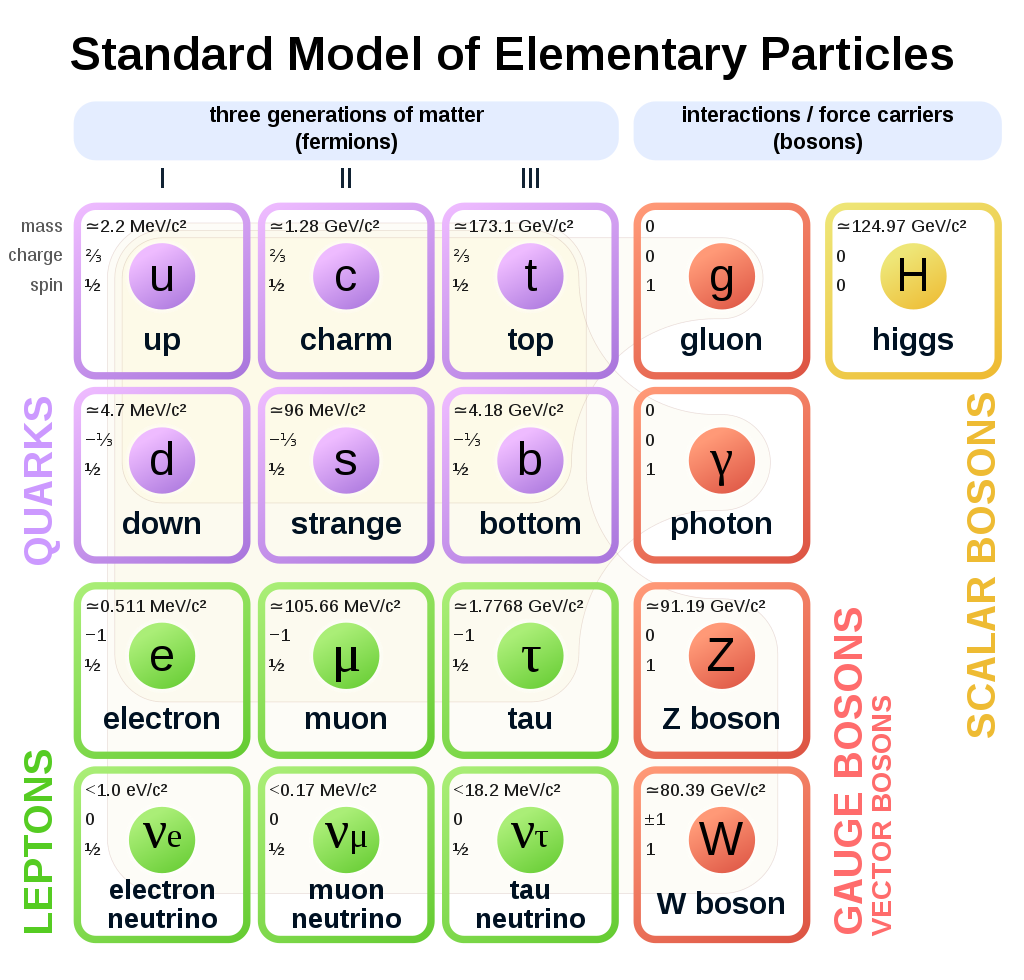
\includegraphics[width=0.7\textwidth]{Images/standard_model.png}
    \caption{The Standard Model.}
    \label{fig:standard_model}
\end{figure*}

In this model, known as the Standard Model, we describe the universe as a composition of particles and the forces between them~\cite{Griffiths}. The leptons, shown in green, include the well-known electron, as well as its nearly-invisible partner, the electron neutrino. Quarks, shown in purple, include the building blocks of protons and neutrons, the up and down quarks. Furthermore, there are the heavier generations of the well-known leptons and quarks, which are just like the electron, electron neutrino, up quark, and down quark, only with more mass. We also have the force carriers (or gauge bosons) in orange - photons for the electromagnetic force, gluons for the strong force, and W and Z bosons for the weak force. Finally, completing the picture is the recently-discovered Higgs boson, an excitation of the Higgs field which gives mass to the other fundamental particles. There are also the antimatter counterparts to these particles, which have opposite charge, though the neutral force carriers are their own antiparticles. The neutrinos may be their own antiparticles too, but whether they are or not is currently the subject of research.

These particles and force carriers, along with the ways in which they are allowed to interact, or "couple" with each other, determine the motion and interaction of all things that we know about in our everyday existence. However, this model is still far from complete, as it does not describe gravity, and is also unable to explain many types of observed astronomical phenomena. Furthermore, there are problems with fine-tuned variables which exist in the model. All of these problems will be described in the next section.

For now though, let's turn our attention to the force carrier particles. These particles are \textbf{describe mixing through electroweak spontaneous symmetry breaking}. This distinction will be important later when we describe supersymmetric extensions to the Standard Model.

\section{Problems with the Standard Model}

The Standard Model has produced some of the most accurate agreements between theory and experiment ever achieved in science, but we know that it does not describe the entire universe. For instance, the Standard Model does not account for dark matter. To clarify, we know from gravitational studies that the amount of invisible matter (matter which does not interact with photons) in the universe is about five times the amount of visible matter. We know this dark matter can not be formed from the charged components of the Standard Model, since these particles all couple to photons. Neutrinos also can not compose more than $10\%$ of dark matter. This is because neutrinos are nearly massless and thus would have been relativistic during the early formation of the universe (assuming they were in thermal equilibrium with everything else). This is inconsistent with the amount of non-relativistic "cold" dark matter which would have been required for structure formation in the universe ~\cite{structure_formation}. Furthermore, there is the proposed existence of dark energy, which is necessary to explain the expansion of the universe, and which is not composed of either matter or dark matter. In total, as seen in Figure~\ref{fig:universe_composition}, ordinary matter and antimatter only account for about $5\%$ of the mass in the universe. Dark matter is $24\%$, and the remaining $71\%$ is dark energy. The Standard Model currently seems incapable of explaining these extra components.

\begin{figure}[htbp]
    \centering
    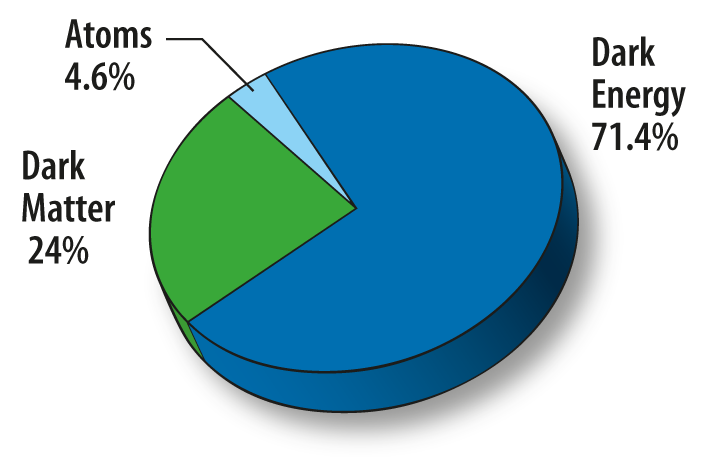
\includegraphics[width=0.7\textwidth]{Images/universe_composition.png}
    \caption{To the best of our knowledge, the universe is composed of $5\%$ ordinary matter, $24\%$ dark matter, and $71\%$ dark energy. The Standard Model describes only ordinary matter, providing one indication that the model is not complete. Image altered from~\cite{universe_composition}.}
    \label{fig:universe_composition}
\end{figure}

Another problem is that gravity is not included in the Standard Model. Gravity is currently the least-understood fundamental force, and many questions about it remain to be answered, such as why gravity is so many orders of magnitude weaker than all the other forces. Attempts to unite the Standard Model with relativistic theories of gravity, as well as attempts to explain the relative weakness of gravity, has led to the development of fields such as string theory.

There is also the Higgs hierarchy problem, which relates to why the Higgs boson has the mass that it does~\cite{SUSY_primer}. To explain, let's say a particle has a certain "bare" mass. As it propagates through space, it interacts with other fields and particles in its environment, causing it to appear to have a different effective mass. Furthermore, in quantum interactions, particles are allowed to interact via "loops". In Figure~\ref{fig:quantum_loops} we see two particles interacting and then propagating away. In this case it is an acceptable interaction for one of the particles to loop around, so that its endpoint is the same as its start point. This particle is then known as a virtual particle, and the interaction is known as a loop interaction. To put it all together, as a particle propagates through empty space, it interacts with virtual particles via loop interactions, changing its observed mass. This observed mass is equal to the particle's bare mass plus contributions to its mass via loop corrections. If we calculate the expected mass of the Higgs, using what we know about how it interacts with other particles, we find that quantum loop corrections from virtual particles ought to be extremely large, with values around the Planck mass at $m_{Planck} = 10^{18}$ GeV. Some of these corrections are positive (for interactions with bosons) and some are negative (for interactions with fermions). For the Higgs to have an observed mass of 126 GeV, the bare mass and all of its corrections have to cancel each other out with an unnatural precision. This indicates that there is some additional undiscovered mechanism which is constraining the magnitude of the mass corrections.

\begin{figure}[htbp]
    \centering
    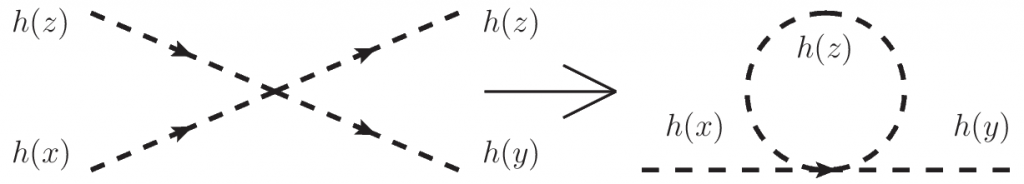
\includegraphics[width=0.9\textwidth]{Images/loop_correction.png}
    \caption{On the left we see two particles interacting, where the x-axis is time. When one of the particles has the same start and end point, as seen on the right, the particle is known as a virtual particle and the interaction is known as a loop interaction. Interactions with virtual particles cause particles to get loop corrections to their observed mass. Image from~\cite{loop_correction}.}
    \label{fig:quantum_loops}
\end{figure}

All of these problems indicate that the Standard Model is not the culmination of physics. There are still things outside the Standard Model which have not yet been discovered. In particular, a class of extensions called supersymmetric (SUSY) theories have been proposed to solve many of the issues described in this section. We will now take a brief look at SUSY in order to understand what the theory proposes and why they are able to shore up various shortcomings of the Standard Model. %[text/images/citations]
\chapter{Supersymmetric Extensions to the Standard Model}

Supersymmetric (SUSY) theories have been proposed as a potential solution to some of the problems described in the previous chapter. According to SUSY~\cite{SUSY_primer}, there is an additional "supersymmetric" partner to each particle that we currently know of. Each boson has a fermionic superpartner, and each fermion has a bosonic superpartner. This simple extension is able to solve the three problems we identified previously.

First, superpartners provide a natural solution to the hierarchy problem. Since each Standard Model fermion and boson has a Higgs mass loop correction which is almost exactly cancelled out by its superpartner, the observed mass of the Higgs boson is able to stay close to zero. Furthermore, if the lightest neutral SUSY particle is incapable of decaying into a normal-matter state, then we would have a long-lived massive particle which does not interact with electromagnetism. This particle could remain undetected and thus would be a candidate for dark matter. In addition, various configurations of string theory state that if SUSY is imposed as a local symmetry then supergravity theories can be formed, merging the Standard Model and general relativity.

With all of these strong points, it would seem that SUSY is a very promising theory. However, despite physicists' best efforts, attempts to search for SUSY particles have so far proved unfruitful. \textbf{History}

Clearly, if SUSY is a correct theory, it must undergo spontaneous symmetry breaking which changes the masses of the undiscovered superpartners, so that e.g. the \textbf{$Z_0$} is not close in mass to its superpartner. Thus it may be that the undiscovered particles are currently outside the energy range of our colliders (though there are upper limits to particle masses before the theory becomes unnatural), or it may be that the particles are too close together in mass, in which case their decay products will be hard to detect. This second possibility will be examined later, and will form part of the motivation for developing our machine-learning based particle identification systems.

\begin{figure}[htbp]
    \centering
    \includegraphics{Images/SUSY.png}
    \caption{Supersymmetric partners of standard-model particles. This diagram displays the squarks, sleptons, and gauginos which make up SUSY. The gauginos (from top to bottom, and left to right) are the gluino, photino, zino, the winos, and the Higgsinos. The photino, zino, and two neutral Higgsinos combine to form mass eigenstates $\tilde{\chi}^0_1, \tilde{\chi}^0_2, \tilde{\chi}^0_3, \tilde{\chi}^0_4$, which are called the neutralinos. The winos and two charged Higgsinos combine to form $\tilde{\chi}^\pm_1, \tilde{\chi}^\pm_2$, the charginos.}
    \label{fig:my_label}
\end{figure}

\textbf{MSSM} %[text/images/citations]

\part{How to Conduct a Particle Physics Experiment}
\chapter{The Detector}

\section{The Layout of CERN}

The Large Hadron Collider (LHC), operated by the CERN collaboration, is a 27-kilometer long proton-proton circular collider located underneath the border area of France and Switzerland, outside the city of Geneva (Figure~\ref{fig:LHC}). The LHC consists of a circular ring, around which two proton beams are accelerated in opposite directions under the guidance of powerful superconducting magnets. These proton beams are allowed to intersect at four beam-crossing points around the ring, where they are smashed head-on at a center-of-mass energy of 13 TeV. There are seven particle detectors stationed around the crossing points to observe the resulting collisions. One of these detectors, ATLAS, is the source of data used in this thesis.

\begin{figure}[htbp]
    \centering
    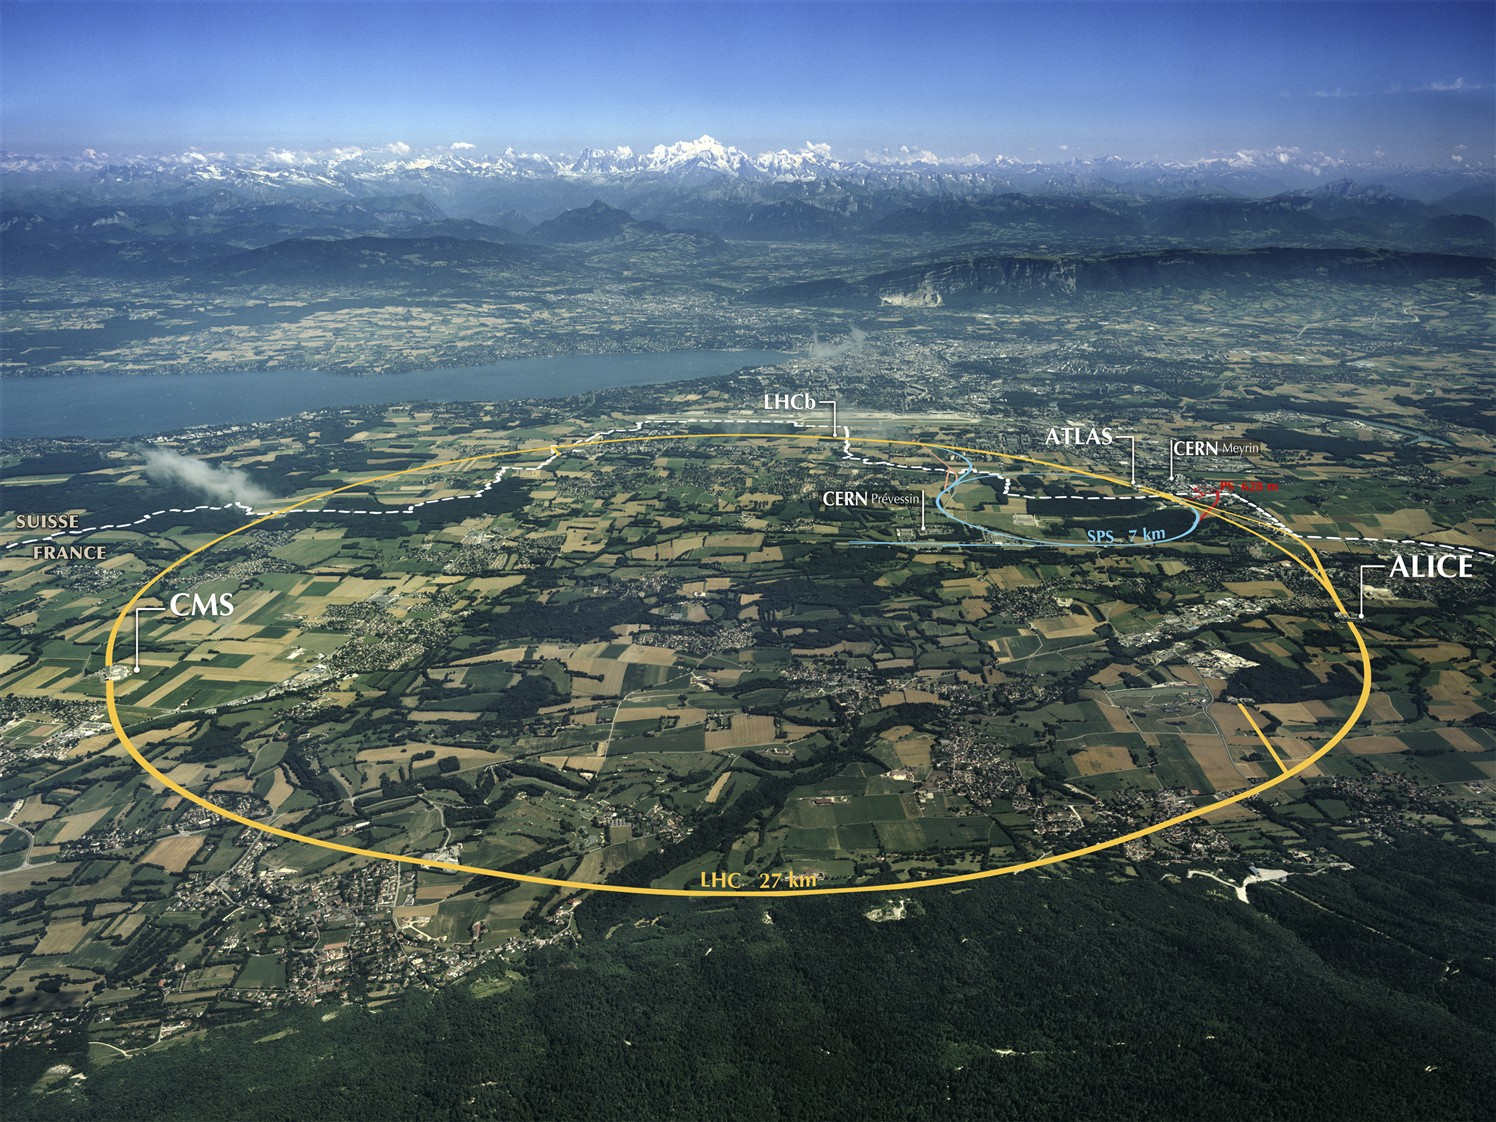
\includegraphics[width=\linewidth]{Images/ATLAS/LHC.jpg}
    \caption{An overhead view of the LHC. Image taken from~\cite{LHC}.}
    \label{fig:LHC}
\end{figure}

\section{An Anatomy of ATLAS}

The ATLAS detector (Figure~\ref{fig:ATLAS}), built around one of the LHC beam crossing points, acts as a eight-story-tall recording device for capturing and digitizing the results of collisions. The detector contains multiple types of detection technology, each specialized to perform a specific type of measurement~\cite{ATLAS_detector}.

\begin{figure}[htbp]
    \centering
    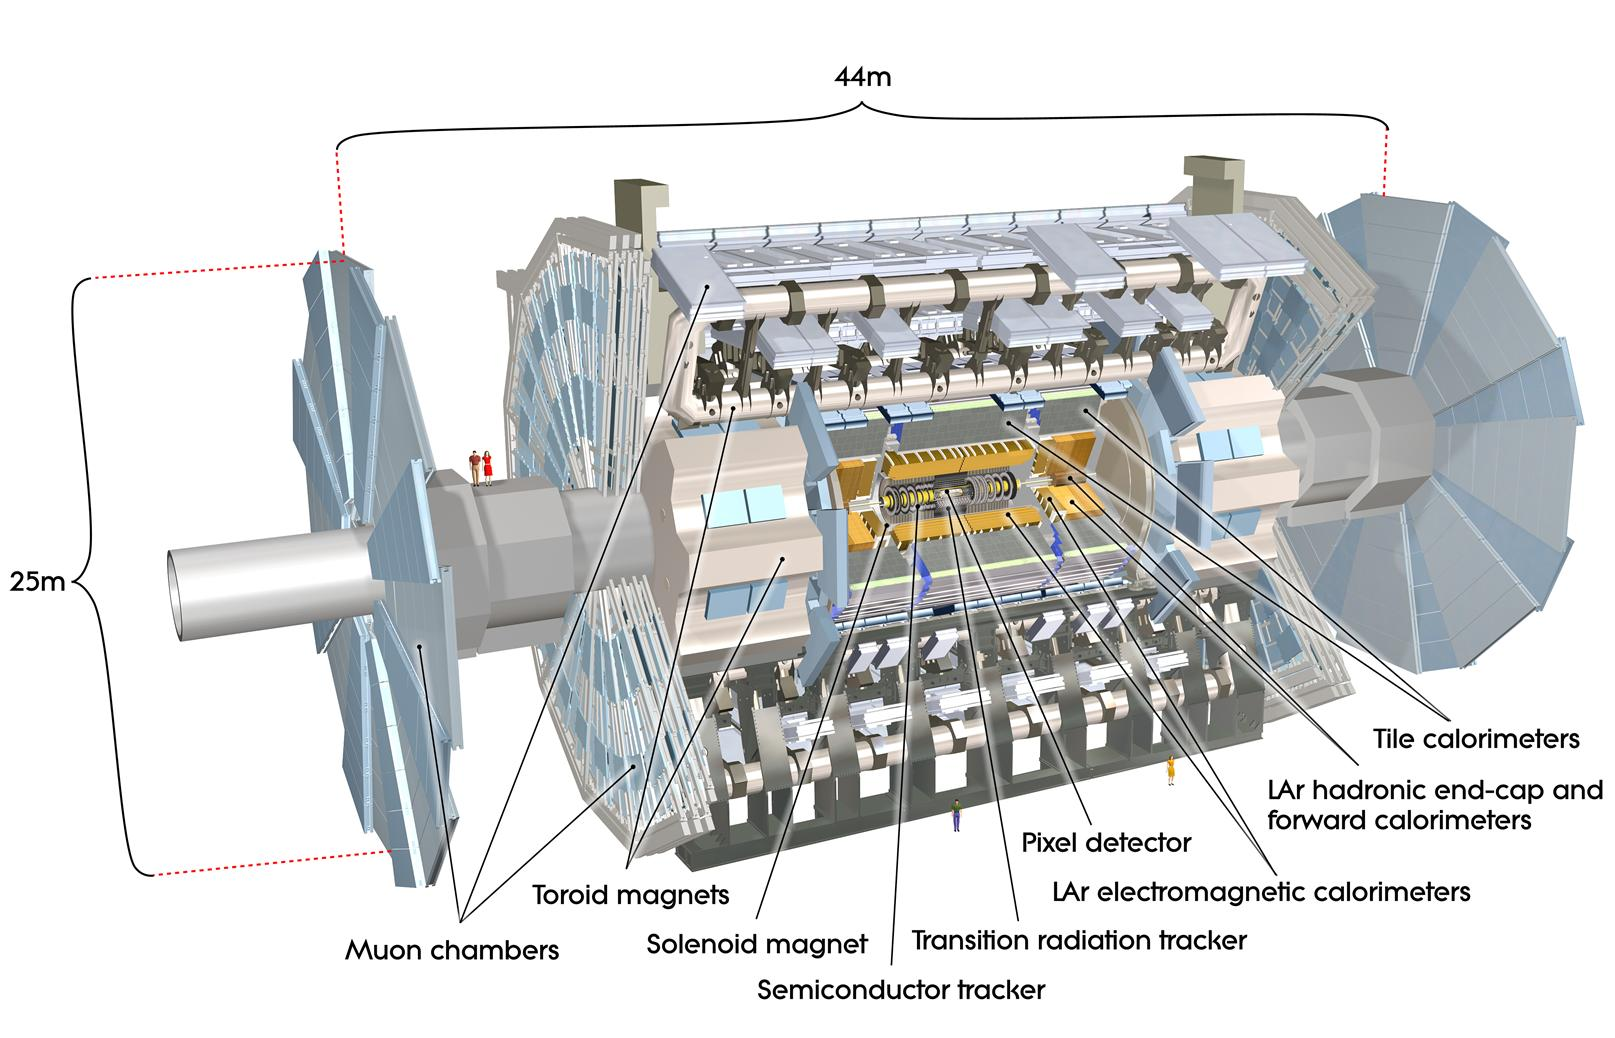
\includegraphics[width=\linewidth]{Images/ATLAS/ATLAS.jpg}
    \caption{A labeled diagram of the ATLAS detector. Figure from~\cite{ATLAS_detector}.}
    \label{fig:ATLAS}
\end{figure}

The backbone of ATLAS consists of a beam pipe surrounded by a solenoid magnet. The protons traverse through the beam pipe and collide, and the resulting particles are curved as they propagate in the plane perpendicular to the beam. Surrounding the beam and the interaction point, we have the inner detector, the calorimeters, and the muon spectrometers (though they have been labelled a bit differently in Figure~\ref{fig:ATLAS}). A partial cross-section view of the detector is shown in Figure~\ref{fig:ATLAS_cross_section}.

\begin{figure}[htbp]
    \centering
    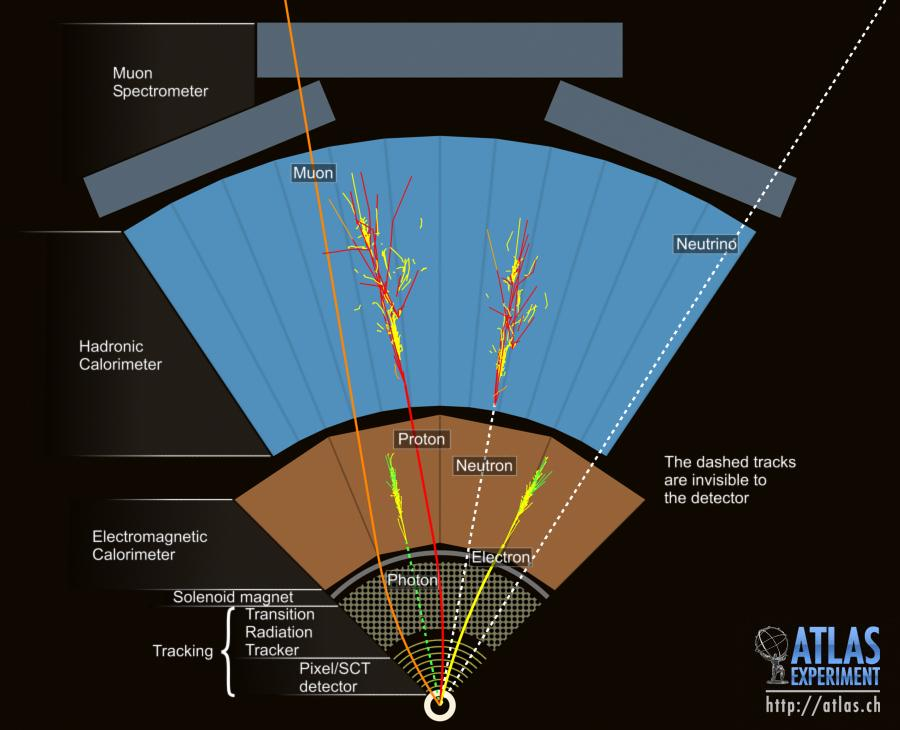
\includegraphics[width=\linewidth]{Images/ATLAS/ATLAS_cross_section.jpg}
    \caption{A cross section of the ATLAS detector. Figure from~\cite{ATLAS_cross_section}.}
    \label{fig:ATLAS_cross_section}
\end{figure}

The inner detector is composed of the silicon pixel and strip detectors and the transition radiation tracker (TRT)~\cite{ATLAS_inner_detector_TDR}. This portion of the detector is used to reconstruct tracks for charged particles, with which we determine their flight paths, momenta, and points of origin. The pixel and strip (SCT) detectors are both silicon-based, and operate via the generation of a depletion region in the material. When charged particles travel through the silicon, they generate electron-hole pairs, which propagate under an applied voltage and are captured via readout chips. The pixel detectors compose the innermost layers, and are segmented finely in both $\eta$ and $\phi$, so as to capture more precise spatial information. The strip detectors are outside the pixel layers, and are segmented only in $\phi$. TRT layers are outside the silicon layers, and consist of Kapton-carbon tubes surrounding tungsten wires. The wires and tubes are kept at a voltage potential, and the space in between is filled with a majority-xenon gas mixture. Once again, passing charged particles ionize the bulk material (in this case the gas), and the resulting electron-hole pairs are captured via the voltage gradient and read out by specialized electronics.

After the inner trackers and the solenoid magnet, we have the calorimeters~\cite{calorimeters_intro}. First we have the electron calorimeter (ECAL), which captures and records the energies of electrons and photons through EM interactions. The hadronic calorimeter (HCAL) is after that, and being composed of heavy elements, it forces hadronic particles to deposit their energies through strong interactions. Each of these calorimeters causes particle showering to occur, during which many charged particles are produced. These particles can then either produce visible photons via scintillation, or produce electron-hole pairs via ionization. The calorimeters are composed of the cylindrical sections concentric to the beam pipe, in what is called the barrel, and the disks on the sides perpendicular to the beam pipe, in what are called the end caps. The ECAL in ATLAS uses liquid argon sampling calorimeters, while the HCAL uses lead and plastic scintillators in the barrel and liquid argon in the endcaps. The ECAL encloses its liquid argon in accordian-like cells, relying on ionization and charge capture, while the HCAL uses alternating planes of lead and plastic, with the lead inducing showering and the plastic capturing the information via scintillation. The deposited energy is determined linearly via the collected signal. The resulting calorimeter energy resolution goes as the following, where $\sigma$ is the resolution, $a$ is statistical due to the number of charged particles produced, $b$ is due to noise and pileup from soft collisions (surrounding collisions, other than the one we're interested in), and $c$ is due to calorimeter errors:

\begin{align}
    \frac{\sigma}{E} &= \frac{a}{\sqrt{E}} \oplus \frac{b}{E} \oplus c
\end{align}

Finally, the detector is ringed by muon spectrometers, which detect the penetrating muons that pass through the rest of the detector~\cite{ATLAS_TDR}. The spectrometers are composed of a barrel section and end caps, and are in charge of precisely measuring the curvature of muons via mechanisms such as drift tubes.

As seen in Figure~\ref{fig:ATLAS_cross_section}, photons and electrons are typically stopped in the ECAL, and protons and neutrons are typically stopped in the HCAL. Charged particles, including electrons, protons, and muons, leave hits in the inner detector. Muons go all the way through the muon detector. Finally, neutrinos pass through ATLAS undetected, and their effects are seen in missing transverse momentum when the transverse momenta of all other decay products in the reaction are summed up. Once all the hits in a single collision are recorded, the data is then passed to triggering and reconstruction algorithms to determine what objects were in the event, and whether or not to store the data.

\section{Upgrades}

The LHC currently produces about 40 collisions per beam-crossing at 13 TeV center-of-mass energy, but with the proposed high-luminosity LHC (HL-LHC) upgrade~\cite{HL_LHC}, there are plans to increase these numbers to 140 collisions per beam-crossing at 14 TeV by 2026, amounting to a total of 250 $fb^{-1}$ of data per year, with ultimate plans to increase to 200 collisions per beam-crossing. During the HL-LHC upgrade, ATLAS similarly plans to upgrade its detection capabilities via the ATLAS Phase-II upgrade~\cite{ATLAS_phaseII_TDR}, focusing on items such as replacing the inner detector with an all-silicon-based inner tracker (ITk), improving data acquisition, and increasing the granularity of calorimeters.

The higher data rates and improved calorimeters provide an incentive to develop and implement the machine-vision based particle identification projects described later in this thesis, and also prompted the lepton isolation machine-learning project which will be described later. Furthermore, in the interest of improving upcoming SUSY searches, I have aided in the development of several other components in the ATLAS detector, including both hardware and firmware upgrades for the inner detector, and vertexing algorithms for event reconstruction. Though these projects are not the focus of this thesis, they will be described in the appendices. %[text/images/citations]
\chapter{The Data}

\section{Object and Event Reconstruction}

\subsection*{Triggers}

\subsection*{Tracks and Vertices}

\subsection*{Physics Objects}

\subsection*{Pileup}

\section{Data and Monte Carlo} %[text/images/citations]
\chapter{How to Do a Search}

\section{What Particle Physicists Do All Day}

\section{Models, Regions, and Backgrounds}\label{sec:background}

\section{Background Estimation}

\section{Interpreting Results}

\subsection*{Unblinding and Comparison}

\subsection*{How to Read Result Plots} %[text/images/citations]

\part{A Search for Supersymmetry}
\chapter{Analysis Details}

We published a paper recently~\cite{SUSY_2l2j} in which we conducted searches using two classes of SUSY models, denoted the strong and electroweak models. Both types of search looked for final products with two opposite-sign same-flavor leptons, at least two jets, and large \MET. These searches used the full ATLAS Run 2 dataset of $\sqrt{s}$ = 13 TeV collision data, with an integrated luminosity of $139 fb^{-1}$. I participated mostly in the strong search, so this is what I will describe here. Some parts of this section have been taken with changes from the paper.

\section{Signal Models}

We looked at three different models in the strong analysis (Figure~\ref{fig:SUSY_models}), which we called gluino-slepton, gluino-$Z^{(*)}$, and squark-$Z^{(*)}$. In these models, we have pair production of hypothesized SUSY particles (either gluino pairs or squark pairs) which decay in certain ways. There are various floating parameters, such as the masses of the SUSY particles, which are partially scanned over in our signal model production grid.

\begin{figure}[htbp]
    \centering
    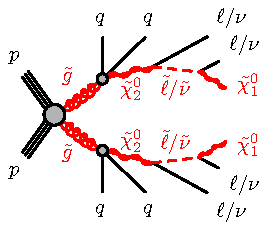
\includegraphics[width=0.32\textwidth]{Images/SUSY/gogo-qqqqllllN1N1-N2.pdf}
    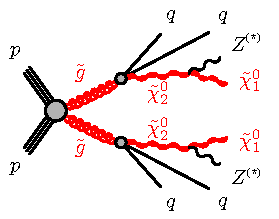
\includegraphics[width=0.32\textwidth]{Images/SUSY/gogo-qqqqZZN1N1.pdf}
    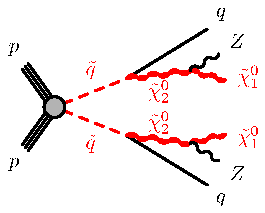
\includegraphics[width=0.32\textwidth]{Images/SUSY/sqsq-qqZZN1N1.pdf}
    \caption{(Left) gluino-slepton model, $\tilde{g}\to qq \tilde{\chi}_2^0$, with $\tilde{\chi}_{2}^{0} \to \tilde{\ell}^{\mp}\ell^{\pm} / \tilde{\nu}\nu$ and $\tilde{\ell}/\tilde{\nu} \to (\ell/\nu)\tilde{\chi}_{1}^{0}$. (Middle) gluino-$Z^{(*)}$ model, $\tilde{g}\to qq \tilde{\chi}_2^0$, with $\tilde{\chi}_2^0\rightarrow Z^{(*)} \tilde{\chi}_1^0$. (Right) squark-$Z^{(*)}$ model, $\tilde{q}\to q \tilde{\chi}_2^0$, with $\tilde{\chi}_2^0\rightarrow Z \tilde{\chi}_1^0$.}
    \label{fig:SUSY_models}
\end{figure}

Each of these models begins with a gluino or squark decaying via quark jets into the second lightest neutralino. These neutralinos then undergo either a two-lepton decay, an on-shell Z decay, or an off-shell Z decay, and end up producing the lightest neutralino, which exits the detector without being detected. Depending on the model, the resulting lepton pairs have different \mll\ distributions. The lightest neutralino, which is also the lightest SUSY particle (LSP) in these models, shows up in our events as \MET.

\section{Signal Production Grids}

In all three models, we consider quark decay or production using five flavors ($u$, $d$, $c$, $s$, $b$) of equal probability. In these simplified models, we ignore all SUSY particles not directly involved in the decay chains, thus considering them to have coupling constants of zero.

As mentioned, the masses of these particles are still unconstrained, so we generate samples in grids over two dimensions, scanning over the LSP mass and either the gluino or squark mass. All squarks are assumed to be mass degenerate in these models. In each case, $\tilde{\chi}_0^2$ is constrained to have a mass halfway between the LSP mass and the mass of the gluino or squark. For example, for the gluino models, $m(\tilde{\chi}_0^2) = [m(\tilde{g})+m(\tilde{\chi^1_0})]/2$. For the slepton model, the masses of the left-handed sleptons are set to $m(\tilde{\ell}) = [m(\tilde{\chi^2_0})+m(\tilde{\chi^1_0})]/2$, while the right-handed sleptons are decoupled.

When the mass difference between $\tilde{\chi}_{2}^{0}$ and $\tilde{\chi}_{1}^{0}$ is less than the $Z$ mass, we have an off-shell model. Otherwise we have an on-Z signal.

The signal samples are produced using MadGraph5 with the NNPDF LO PDF set and contain up to one additional parton in the matrix element. The generation uses Pythia8 for showering and hadronization with EvtGen and the ATLAS A14 tune and the CTEQ 6L1 PDF set in the shower. Decoupled sparticles are vetoed in the production diagrams in MadGraph5. Signal production cross sections are calculated at NNLO$_\text{approx}$ with NNLL resummation. The details of strong signal model generation can be found in the following JIRA tickets~\cite{JIRAGluinoSLN, JIRAGluinoZ, JIRASleptonZ}.

\section{Physics Objects and Processes}

For the purposes of performing jet overlap removal and calculating $E_T^{miss}$, we chose to use baseline leptons with \pt\ above 10 GeV and baseline jets above 20 GeV. In the interest of keeping this paper at a reasonable length, the complete set of object selection and triggering criteria will not be included, but can be found in the complete SUSY analysis paper at \cite{SUSY_2l2j}. These selections included different $\eta$ acceptances for electrons and muons, various requirements on object reconstruction quality and isolation, and cuts on impact parameters. On top of this, our regions used signal leptons with \pt\ above 25 GeV, and jets with \pt\ above 30 GeV.

As with most high-energy physics searches, there were a variety of standard-model processes which mimicked the final state we were looking for. Of these, the $t\bar{t}$ process was the largest, followed by diboson (WZ/ZZ) processes. Events with a single Z and two or more jets from initial-state radiation could also mimic our signal, provided that mismeasurement of the jet momentum resulted in a large \MET\ for the event. Events from single-top-quark processes and from lepton misidentification also contributed to the background. To accurately model these backgrounds, we used flavor-symmetry (FS), Z MC scaling, fake estimation, and Monte Carlo methods, all of which will be described later.

\section{Regions}

When selecting regions for this analysis, we decided to require at least two signal leptons with transverse momentum ($p_T$) above 25 GeV and at least one jet with $p_T$ above 30 GeV in all regions.

As we had several unknown masses in our models, we needed to find multiple signal regions which could optimize the signal-to-background ratio for a variety of different $\tilde{\chi}^0_1$, $\tilde{\chi}^0_2$, and $\tilde{g}$ masses. In Tables~\ref{tab:strongSRDef} and~\ref{tab:strongVRDef}, we describe the strong signal and validation regions we chose.

\begin{table}[htbp]
    \centering
    \begin{tabular}{l|c|c|c|c|c|c|c}
    Preselection & \multicolumn{7}{c}{Lepton triggers} \\
    Preselection & \multicolumn{7}{c}{Lepton \pt$>25$; $==2$ leptons (baseline \& signal) SF-OS } \\
    Preselection & \multicolumn{7}{c}{\mll$>12$} \\
    Preselection & \multicolumn{7}{c}{\ptll$>40$} \\
    Preselection & \multicolumn{7}{c}{Jet \pt$>30$; $\geq2$ jets} \\
    Preselection & \multicolumn{7}{c}{$\Delta\phi(\mathrm{jet}_{1,2},$\MET$)>0.4$} \\
    \hline
    Region & \njet & \HT & \MET & \mttwo & \EtmissSig & \ptll & \mll \\
    \hline
    SRC   & $-$  & $-$    & $>250$ & $>90$ & $>10$ & $<100$  & $-$ \\
    SRLow & $-$  & $>250$ & $>250$ & $>100$ & $-$ & $<500$& $-$   \\
    \quad SRZLow & $\geq4$  & $>250$ & $>250$ & $>100$ & $-$ & $<500$& $81-101$   \\
    SRMed & $-$  & $>500$ & $>300$ & $>75$ & $-$ & $<800$ & $-$   \\
    \quad SRZMed & $\geq4$  & $>500$ & $>300$ & $>75$ & $-$ & $<800$ & $81-101$   \\
    SRHigh& $-$  & $>800$ & $>300$ & $>75$ & $-$ & $-$    & $-$   \\
    \quad SRZHigh& $\geq4$  & $>800$ & $>300$ & $>75$ & $-$ & $-$    & $81-101$  \\
    \end{tabular}
    \caption{Strong signal regions, with units in GeV. When Z regions are used as control regions for FS estimates, the \mll\ window is expanded to 61--121 GeV.}
    \label{tab:strongSRDef}
\end{table}

\begin{table}[htbp]
    \centering
    \begin{tabular}{l|c|c|c|c|c|c|c}
    Preselection & \multicolumn{7}{c}{Same as SRs} \\
    \hline
    Region & \njet & \HT & \MET & \mttwo & \EtmissSig & \ptll & \mll \\
    \hline
    VRC    & $-$  & $-$    & $\bm{150-250}$ & $>90$ & $>10$ & $<100$  & $-$ \\
    VRLow  & $-$  & $>250$ & $\bm{150-250}$ & $>100$ & $-$ & $<500$& $-$   \\
    VRMed  & $-$  & $>500$ & $\bm{150-250}$ & $>75$ & $-$ & $<800$ & $-$   \\
    VRHigh & $-$  & $>800$ & $\bm{150-250}$ & $>75$ & $-$ & $-$    & $-$   \\
    \hline\hline
    Preselection & \multicolumn{7}{c}{Same as SRs but} \\
    Preselection & \multicolumn{7}{c}{\textbf{3 Leptons} (baseline+signal)} \\
    \hline
    Region & \njet & \HT & \MET & \mttwo & \EtmissSig & \ptll & \mll \\
    \hline
    VR3L  & $-$  & $>250$ & $\bm{>200}$ & $>100$ & $-$ & $-$& $-$   \\
    \hline\hline
    Preselection & \multicolumn{7}{c}{Same as SRs but} \\
    Preselection & \multicolumn{7}{c}{\textbf{Same Sign Leptons}} \\
    Preselection & \multicolumn{7}{c}{\textbf{SF+DF Leptons}} \\
    \hline
    Region & \njet & \HT & \MET & \mttwo & \EtmissSig & \ptll & \mll \\
    \hline
    VRSS  & $-$  & $>250$ & $\bm{>150}$ & $>75$ & $-$ & $\bm{-}$& $-$   \\
    \end{tabular}
    \caption{Strong validation regions, with units in GeV.  Differences from SRs are highlighted in bold.}
    \label{tab:strongVRDef}
\end{table} %[text/images/citations]
\chapter{Sample Production Details}

There's a lot of tuning which goes into sample production, involving things like trigger selections, MC validation checks, and of course writing code and creating bug fixes. There is a lot of work that goes into sample production (most of which is quite boring), but here I'm just going to talk about a few of the studies I did.

\section{Lepton Triggers}

One thing that goes into sample production is the selection of the trigger menu. We want to make sure that we choose triggers which capture most of the interesting objects, while not allowing an overwhelming amount of data to be present in our samples. Of course, we also select in such a way that the signal over background ratio for physics objects is maximized.

Here I show differences between four sets of trigger selections. First I describe the triggers that go into each menu, and then I compare trigger results in three different regions.

The trigger menus I will compare here are labelled 'trigMatch\_1L2LTrig', 'trigMatch\_1L2LTrigOR', 'trigMatch\_2LTrig', and 'trigMatch\_2LTrigOR'. The difference between 1L2LTrig and 2LTrig menus is that 1L2LTrig menus contain both single-lepton triggers like HLT\_e60\_medium and two-lepton triggers like HLT\_2mu10 while the 2LTrig menus only contain the two-lepton triggers. The difference between OR and non-OR menus is that the non-OR menus use the lowest unprescaled triggers in each run, while the OR menus use all triggers over all runs. The OR triggers are easier to implement and debug. Low-\pt\ isolated single-lepton triggers are not included, since they would bias the estimation of fake leptons using the matrix method (as will be described in the next chapter). High-\pt\ non-isolated single-lepton triggers are also not included, since they make scale factor calculation more complicated, and were found not to increase signal acceptance by very much.

Using data and a selection of signal samples (taken from an electroweak model sample grid), we look at trigger efficiencies in several regions. In Tables~\ref{tab:trigger_first} to~\ref{tab:trigger_last} we quote the percentage of events which pass each trigger in each region, using all events in that region (with no trigger requirement) as a baseline. We found that 2LTrigOR was a good menu to use, as it maintained a good signal over background ratio, while being the simplest to implement. Values in these tables are labelled `nan` when there are no passing events.

\begin{table}
\begin{center}
\caption{trigMatch\_1L2LTrig Efficiency in SR Low Region (\%)}
\begin{tabular}{l|l|l}
& ee & mm \\
\hline
data15-16 & 100 & 93.9655 \\
data17 & 82.6087 & 84.507 \\
data18 & 91.3044 & 79.375 \\
(600, 0) MC16a & 100 & 100 \\
(600, 0) MC16cd & 100 & 100 \\
(600, 0) MC16e & 100 & 83.3333 \\
(200, 100) MC16a & -nan & -nan \\
(200, 100) MC16cd & -nan & -nan \\
(200, 100) MC16e & -nan & -nan
\label{tab:trigger_first}
\end{tabular}
\end{center}
\end{table}

\begin{table}
\begin{center}
\caption{trigMatch\_1L2LTrigOR Efficiency in SR Low Region (\%)}
\begin{tabular}{l|l|l}
& ee & mm \\
\hline
data15-16 & 100 & 95.6897 \\
data17 & 82.6087 & 97.1831 \\
data18 & 91.3044 & 96.25 \\
(600, 0) MC16a & 100 & 100 \\
(600, 0) MC16cd & 100 & 100 \\
(600, 0) MC16e & 100 & 100 \\
(200, 100) MC16a & -nan & -nan \\
(200, 100) MC16cd & -nan & -nan \\
(200, 100) MC16e & -nan & -nan \\
\end{tabular}
\end{center}
\end{table}

\begin{table}
\begin{center}
\caption{trigMatch\_2LTrig Efficiency in SR Low Region (\%)}
\begin{tabular}{l|l|l}
& ee & mm \\
\hline
data15-16 & 84.6154 & 90.5172 \\
data17 & 78.2609 & 92.9577 \\
data18 & 65.2174 & 93.125 \\
(600, 0) MC16a & 100 & 100 \\
(600, 0) MC16cd & 66.6667 & 88.8889 \\
(600, 0) MC16e & 100 & 100 \\
(200, 100) MC16a & -nan & -nan \\
(200, 100) MC16cd & -nan & -nan \\
(200, 100) MC16e & -nan & -nan \\
\end{tabular}
\end{center}
\end{table}

\begin{table}
\begin{center}
\caption{trigMatch\_2LTrigOR Efficiency in SR Low Region (\%)}
\begin{tabular}{l|l|l}
& ee & mm \\
\hline
data15-16 & 84.6154 & 90.5172 \\
data17 & 78.2609 & 92.9577 \\
data18 & 65.2174 & 93.125 \\
(600, 0) MC16a & 100 & 100 \\
(600, 0) MC16cd & 66.6667 & 88.8889 \\
(600, 0) MC16e & 100 & 100 \\
(200, 100) MC16a & -nan & -nan \\
(200, 100) MC16cd & -nan & -nan \\
(200, 100) MC16e & -nan & -nan \\
\end{tabular}
\end{center}
\end{table}

\begin{table}
\begin{center}
\caption{trigMatch\_1L2LTrig Efficiency in SR Medium Region (\%)}
\begin{tabular}{l|l|l}
& ee & mm \\
\hline
data15-16 & 100 & 92.4242 \\
data17 & 86.2069 & 88 \\
data18 & 97.7273 & 83.0769 \\
(600, 0) MC16a & 99.6942 & 98.5795 \\
(600, 0) MC16cd & 99.6528 & 97.2973 \\
(600, 0) MC16e & 99.6169 & 96.3636 \\
(200, 100) MC16a & -nan & 100 \\
(200, 100) MC16cd & 100 & 100 \\
(200, 100) MC16e & 100 & -nan \\
\end{tabular}
\end{center}
\end{table}

\begin{table}
\begin{center}
\caption{trigMatch\_1L2LTrigOR Efficiency in SR Medium Region (\%)}
\begin{tabular}{l|l|l}
& ee & mm \\
\hline
data15-16 & 100 & 93.9394 \\
data17 & 86.2069 & 96 \\
data18 & 97.7273 & 91.5385 \\
(600, 0) MC16a & 100 & 98.8636 \\
(600, 0) MC16cd & 99.6528 & 99.6997 \\
(600, 0) MC16e & 99.6169 & 99.0909 \\
(200, 100) MC16a & -nan & 100 \\
(200, 100) MC16cd & 100 & 100 \\
(200, 100) MC16e & 100 & -nan \\
\end{tabular}
\end{center}
\end{table}

\begin{table}
\begin{center}
\caption{trigMatch\_2LTrig Efficiency in SR Medium Region (\%)}
\begin{tabular}{l|l|l}
& ee & mm \\
\hline
data15-16 & 91.6667 & 90.9091 \\
data17 & 79.3103 & 92 \\
data18 & 84.0909 & 86.1538 \\
(600, 0) MC16a & 97.5535 & 97.1591 \\
(600, 0) MC16cd & 94.4444 & 96.6967 \\
(600, 0) MC16e & 94.636 & 97.5758 \\
(200, 100) MC16a & -nan & 100 \\
(200, 100) MC16cd & 100 & 100 \\
(200, 100) MC16e & 100 & -nan \\
\end{tabular}
\end{center}
\end{table}

\begin{table}
\begin{center}
\caption{trigMatch\_2LTrigOR Efficiency in SR Medium Region (\%)}
\begin{tabular}{l|l|l}
& ee & mm \\
\hline
data15-16 & 95.8333 & 90.9091 \\
data17 & 79.3103 & 92 \\
data18 & 84.0909 & 86.1538 \\
(600, 0) MC16a & 97.5535 & 97.1591 \\
(600, 0) MC16cd & 94.4444 & 96.6967 \\
(600, 0) MC16e & 94.636 & 97.5758 \\
(200, 100) MC16a & -nan & 100 \\
(200, 100) MC16cd & 100 & 100 \\
(200, 100) MC16e & 100 & -nan \\
\end{tabular}
\end{center}
\end{table}

\begin{table}
\begin{center}
\caption{trigMatch\_1L2LTrig Efficiency in SR High Region (\%)}
\begin{tabular}{l|l|l}
& ee & mm \\
\hline
data15-16 & 100 & 92.3077 \\
data17 & 100 & 72.7273 \\
data18 & 50 & 57.1429 \\
(600, 0) MC16a & 100 & 94.1176 \\
(600, 0) MC16cd & 100 & 90.9091 \\
(600, 0) MC16e & 90 & 100 \\
(200, 100) MC16a & -nan & -nan \\
(200, 100) MC16cd & -nan & -nan \\
(200, 100) MC16e & 100 & -nan \\
\end{tabular}
\end{center}
\end{table}

\begin{table}
\begin{center}
\caption{trigMatch\_1L2LTrigOR Efficiency in SR High Region (\%)}
\begin{tabular}{l|l|l}
& ee & mm \\
\hline
data15-16 & 100 & 92.3077 \\
data17 & 100 & 81.8182 \\
data18 & 50 & 66.6667 \\
(600, 0) MC16a & 100 & 94.1176 \\
(600, 0) MC16cd & 100 & 90.9091 \\
(600, 0) MC16e & 90 & 100 \\
(200, 100) MC16a & -nan & -nan \\
(200, 100) MC16cd & -nan & -nan \\
(200, 100) MC16e & 100 & -nan \\
\end{tabular}
\end{center}
\end{table}

\begin{table}
\begin{center}
\caption{trigMatch\_2LTrig Efficiency in SR High Region (\%)}
\begin{tabular}{l|l|l}
& ee & mm \\
\hline
data15-16 & 100 & 92.3077 \\
data17 & 100 & 81.8182 \\
data18 & 50 & 66.6667 \\
(600, 0) MC16a & 100 & 94.1176 \\
(600, 0) MC16cd & 85.7143 & 90.9091 \\
(600, 0) MC16e & 90 & 100 \\
(200, 100) MC16a & -nan & -nan \\
(200, 100) MC16cd & -nan & -nan \\
(200, 100) MC16e & 100 & -nan \\
\end{tabular}
\end{center}
\end{table}

\begin{table}
\begin{center}
\caption{trigMatch\_2LTrigOR Efficiency in SR High Region (\%)}
\begin{tabular}{l|l|l}
& ee & mm \\
\hline
data15-16 & 100 & 92.3077 \\
data17 & 100 & 81.8182 \\
data18 & 50 & 66.6667 \\
(600, 0) MC16a & 100 & 94.1176 \\
(600, 0) MC16cd & 85.7143 & 90.9091 \\
(600, 0) MC16e & 90 & 100 \\
(200, 100) MC16a & -nan & -nan \\
(200, 100) MC16cd & -nan & -nan \\
(200, 100) MC16e & 100 & -nan
\label{tab:trigger_last}
\end{tabular}
\end{center}
\end{table}

\section{MC Angle Validation Plots}

Part of MC validation involves checking for any deadspots or hotspots in the 2D eta-phi angle space~\cite{twiki_checks} for leading jets and leptons. Any large peaks or dips would demonstrate an issue in the sample production process. To do these checks, I created plots for our various sample processes in each of our strong and electroweak regions.

A random selection of these plots are shown in Figures~\ref{fig:MC_angle_validation_first} to~\ref{fig:MC_angle_validation_last}. Examining these plots demonstrated that there were no issues in this particular case.

\begin{figure}[htbp]
\centering
\begin{minipage}{0.45\textwidth}
    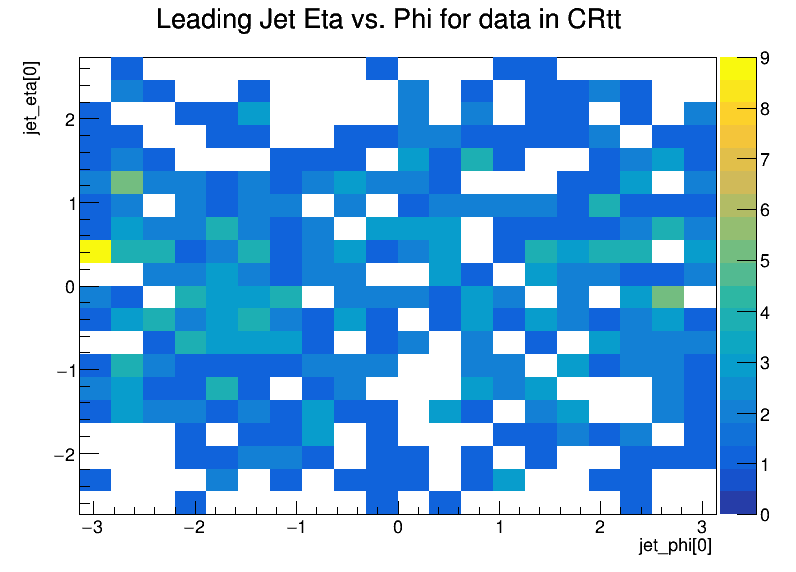
\includegraphics[width=\textwidth]{Images/SUSY/jet_eta_phi_data_CRtt.png}
    \caption{$\eta$ vs $\phi$ plot for leading jets for data in CRtt.}
    \label{fig:MC_angle_validation_first}
\end{minipage}
\hfill
\begin{minipage}{0.45\textwidth}
    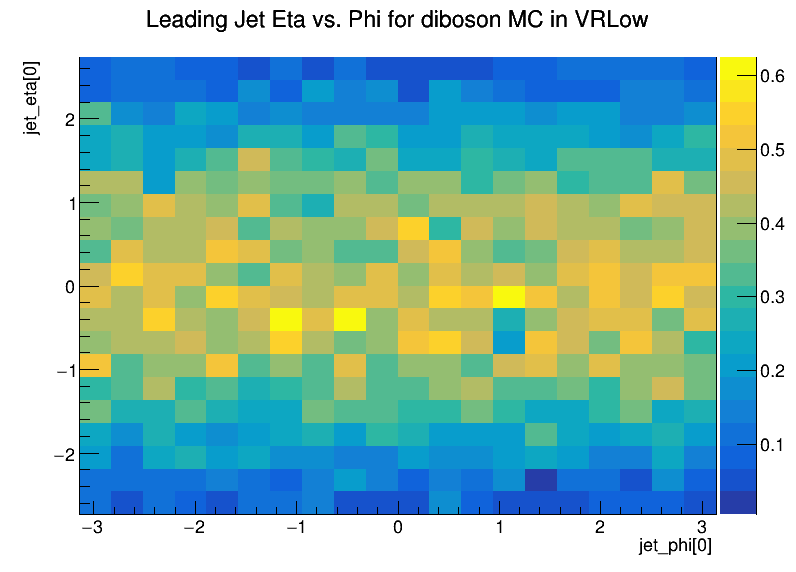
\includegraphics[width=\textwidth]{Images/SUSY/jet_eta_phi_diboson_VRLow.png}
    \caption{$\eta$ vs $\phi$ plot for leading jets for diboson in VRLow.}
\end{minipage}
\end{figure}

\begin{figure}[htbp]
\centering
\begin{minipage}{0.45\textwidth}
    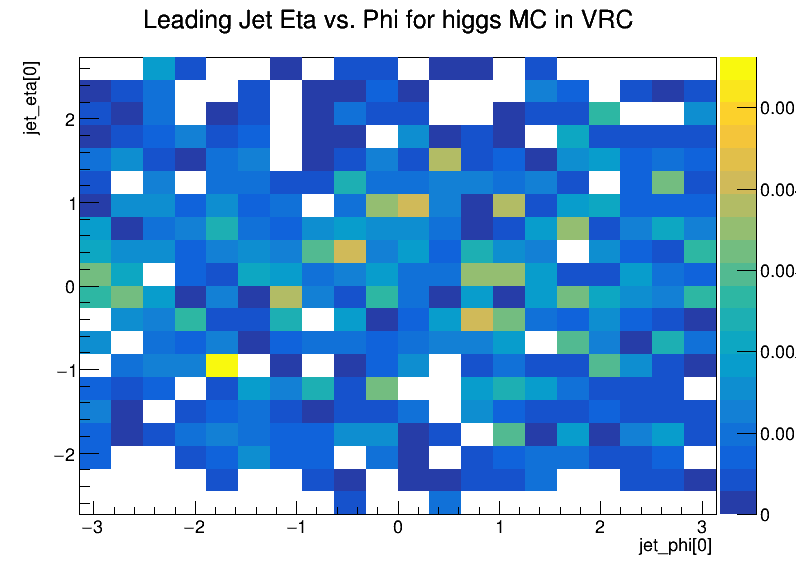
\includegraphics[width=\textwidth]{Images/SUSY/jet_eta_phi_higgs_VRC.png}
    \caption{$\eta$ vs $\phi$ plot for leading jets for higgs in VRC.}
\end{minipage}
\hfill
\begin{minipage}{0.45\textwidth}
    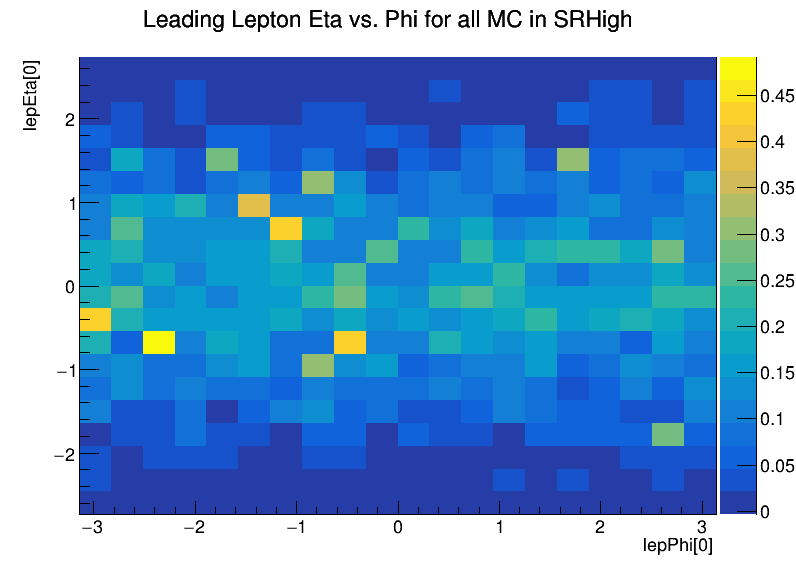
\includegraphics[width=\textwidth]{Images/SUSY/lep_eta_phi_all_MC_SRHigh.png}
    \caption{$\eta$ vs $\phi$ plot for leading leptons for all MC in SRHigh.}
\end{minipage}
\end{figure}

\begin{figure}[htbp]
\centering
\begin{minipage}{0.45\textwidth}
    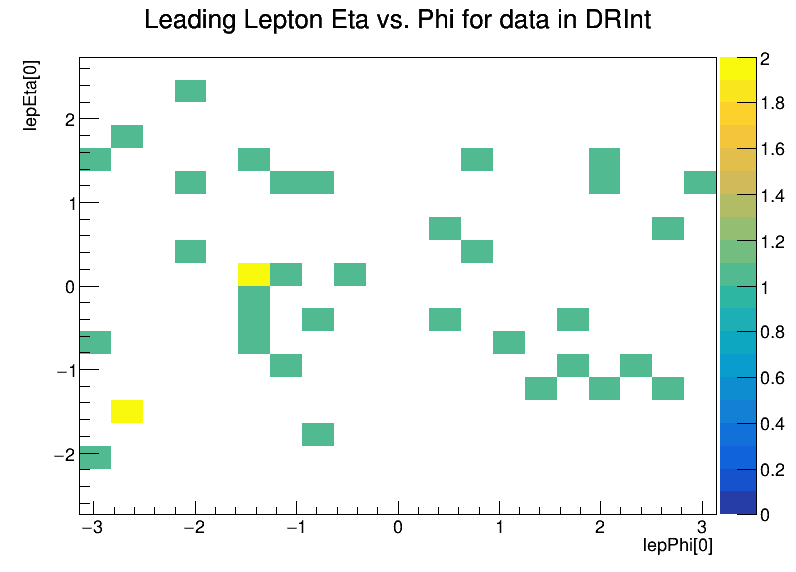
\includegraphics[width=\textwidth]{Images/SUSY/lep_eta_phi_data_DRInt.png}
    \caption{$\eta$ vs $\phi$ plot for leading leptons for data in DRInt.}
\end{minipage}
\hfill
\begin{minipage}{0.45\textwidth}
    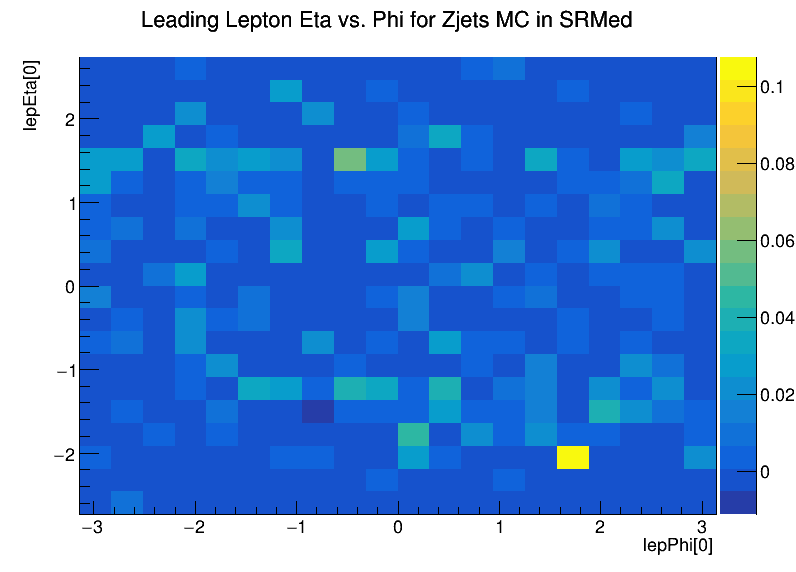
\includegraphics[width=\textwidth]{Images/SUSY/lep_eta_phi_Zjets_SRMed.png}
    \caption{$\eta$ vs $\phi$ plot for leading lepton for Zjets in SRMed.}
    \label{fig:MC_angle_validation_last}
\end{minipage}
\end{figure}

\section{Photon Overlap Removal}

Another issue we had to check was the use of overlap removal in sample production. After the photon method (to be described later) was shown to be problematic, we turned off photon-based overlap removal for the next set of samples. Here I show that this choice did not have a significant impact on relevant Z and data samples.

To do this, I checked a subset of samples for Z MC and data. I produced these samples with and without the OR.DoPhoton flag, and plotted the \MET\ distributions against each other. These plots, shown in Figures~\ref{fig:ORPhoton_first} to~\ref{fig:ORPhoton_last}, demonstrates that turning off photon overlap removal does not have much impact.

The samples used are the following:

\begin{itemize}
    \item \seqsplit{mc16\_13TeV.364121.Sherpa\_221\_NNPDF30NNLO\_Zee\_MAXHTPTV140\_280\_CFilterBVeto.deriv.DAOD\_SUSY2.e5299\_s3126\_r10724\_p4189}
    \item \seqsplit{mc16\_13TeV.364102.Sherpa\_221\_NNPDF30NNLO\_Zmumu\_MAXHTPTV0\_70\_BFilter.deriv.DAOD\_SUSY2.e5271\_s3126\_r10201\_p4189}
    \item \seqsplit{data18\_13TeV.periodB.physics\_Main.PhysCont.DAOD\_SUSY2.grp18\_v01\_p3991}.
\end{itemize}

\begin{figure}[htbp]
\centering
\begin{minipage}{0.45\textwidth}
    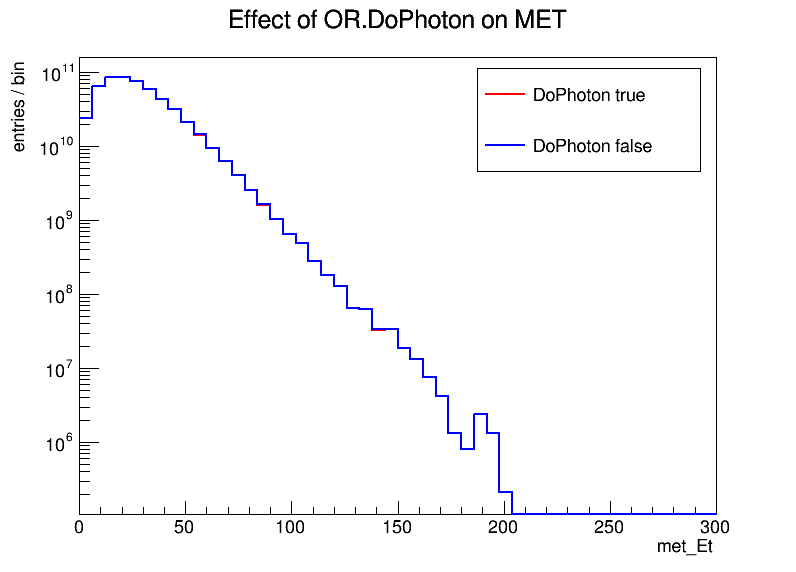
\includegraphics[width=\textwidth]{Images/SUSY/ORDoPhoton_Zee.png}
    \caption{\MET\ with and without photon overlap removal for Zee.}
    \label{fig:ORPhoton_first}
\end{minipage}
\hfill
\begin{minipage}{0.45\textwidth}
    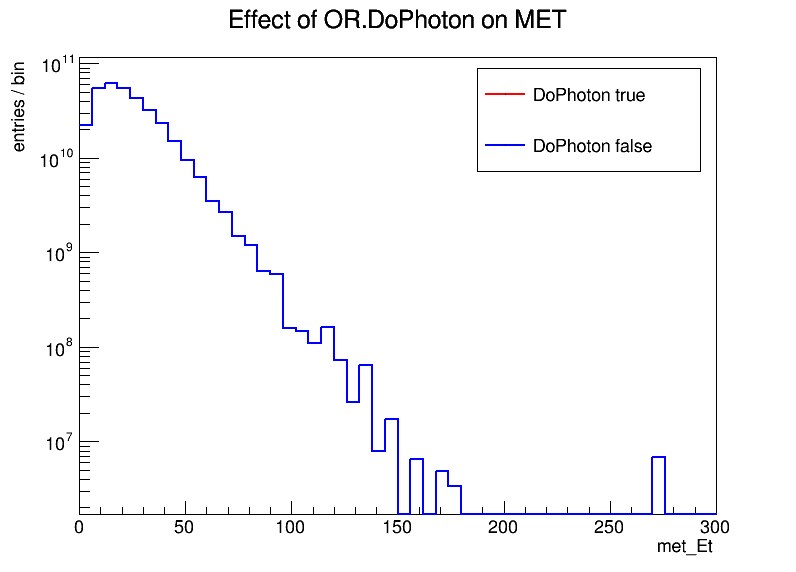
\includegraphics[width=\textwidth]{Images/SUSY/ORDoPhoton_Zmm.png}
    \caption{\MET\ with and without photon overlap removal for Zmm.}
\end{minipage}
\end{figure}

\begin{figure}[htbp]
    \centering
    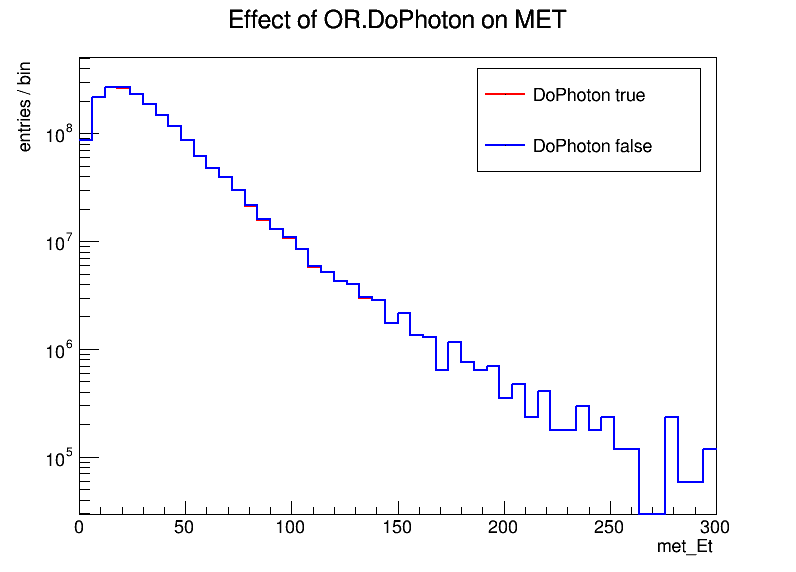
\includegraphics[width=0.45\textwidth]{Images/SUSY/ORDoPhoton_data.png}
    \caption{\MET\ with and without photon overlap removal for data.}
    \label{fig:ORPhoton_last}
\end{figure} %[citations]
\section{Backgrounds}

Here we briefly describe the major backgrounds in our analysis. I was in charge of the Z background estimation, as will be discussed in the next section. I also provided theory systematic uncertainties for the MC components of both the Strong and Electroweak analyses.

\subsection*{Flavor Symmetry}

We used the flavor symmetry method to remove contributions from processes such as $Z\rightarrow\tau\tau$, $t\tilde{t}$, WW, and tW. Unlike our signal models, which produced only pairs of same-flavor leptons, these processes could produce same-flavor and opposite-flavor lepton pairs with equal probability. The basic idea was to take the opposite-flavor $e\mu$ events from data in each signal region, and to use them to estimate the number of same-flavor events from FS sources in each of those regions. Due to differences in detection and triggering efficiencies for electrons and muons, we had to apply the scaling factor shown in the following equation, where $\epsilon_{e/\mu}$ was the offline selection efficiency for each lepton and $\epsilon_{e\mu/ee}^{trigger}$ was the dilepton trigger efficiency for each channel. The equation for the $\mu\mu$ channel followed the same logic.

\begin{gather}
n_{ee}^{measured} = \frac{1}{2}\frac{\epsilon_e}{\epsilon_{\mu}}\frac{\epsilon_{ee}^{trigger}}{\epsilon_{e\mu}^{trigger}}n_{e\mu}^{measured}
\end{gather}

\subsection*{Z/$\gamma^*$ + Jets}

In our Z+jets backgrounds, the majority of our missing energy comes from jet mismeasurements. Since Monte Carlo has trouble accurately simulating the QCD processes involved in jet processes, we use a data-based method to estimate this component of the background. This method has been used before in physics searches in both CMS and ATLAS.

\subsection*{Fake Leptons}

Another contribution to background came from events where one or more non-leptonic objects were incorrectly identified as leptons. Semileptonic $t\bar{t}$, W + jets, and single top events were included in this category. We estimated the number of fake leptons in each region using a matrix method described in detail in \cite{fake_method}. The general idea was that in each signal region, we would apply both loose and tight lepton selections. We labeled the number of baseline (loose) leptons which passed the signal (tight) cut as $N_{pass}$, and called the ones which failed $N_{fail}$. Given two further numbers, $\epsilon^{real}$ and $\epsilon^{fake}$ (fractions which pass the signal cut), we could then estimate the number of fake signal leptons using the following equation. $\epsilon^{real}$ and $\epsilon^{fake}$ were calculated via a tag-and-probe approach. Expanding this method to a dilepton system (where either or both leptons could be fake) required only that we extend this logic to a 4x4 matrix.

\begin{equation}
N_{pass}^{fake} = \frac{N_{fail}-(1/\epsilon^{real}-1)\times N_{pass}}{1/\epsilon^{fake}-1/\epsilon^{real}}.
\end{equation}

\subsection*{Monte Carlo}

Other small components were modelled using MC. %[citations]
\chapter{Z Background Estimation}

We describe here two methods of estimating $Z\rightarrow\ell\ell$ backgrounds in our Strong SUSY regions. The first method relies on the statistical manipulation of data-driven photon+jets backgrounds, and has been used in our previous analyses. We describe this method, and show that it is inapplicable to our current analysis due to violation of several underlying method assumptions. The second method we describe, based on the scaling of Z Monte Carlo samples to a \mindphijm\ control region for each signal and validation region, is the one we use for our current analysis. We show that this method replicates important features accurately, and is robust to theory systematic variations.

\section{Photon Method}

In our Z+jets backgrounds, the majority of our missing energy comes from jet mismeasurements. We first investigated a data-driven method to estimate this component of the background, as it has been used before in physics searches in both CMS and ATLAS ~\cite{blah}, including in one of our previous analyses ~\cite{blah}.

This method involves selecting photon+jets events from data, and applying corrections in order to simulate Z+jets events (Figure~\ref{fig:photon_to_Z}). The method works because the two types of processes have very similar jet behavior, allowing us to use a data-driven method for estimating jets, rather than relying on tricky QCD-based simulation in Monte Carlo.

\begin{figure}
    \centering
    %\includegraphics{}
    \caption{Caption}
    \label{fig:photon_to_Z}
\end{figure}

The major differences between Z+jets and photon+jets events come from the presence of leptonic components, which can be simulated by pseudo-splitting the photon into two leptons. From looking at photon and Z events in MC, we apply corrections to each photon event to produce a lepton splitting similar to what is seen in an equivalent Z event of the same transverse momentum. To be more specific, we first split the photon into two leptons according to a uniform angle sampling on the unit sphere in the rest frame of the photon. We then boost the daughter leptons back to the lab frame. This lepton splitting causes our first problem, as will be described in the next section.

After splitting the photon into leptons, we must then perform a resolution smearing procedure to account for the fact that photons and leptons have different measurement resolutions within our detector. [describe how method works, and how we then smear the pT of the photon based on resulting lepton pT]. [In particular, there is significant mismeasurement of muons at high pT. This leads to differences in MET distibutions. To simplify calculations, we treat lepton propagation as mostly being in the direction of Z propagation. Thus our smearing method only affects MET in the direction parallel to the direction of Z propagation (METl), and not in the transverse direction (METt). To apply smearing, we look at METl in slices of pT for both photon and Z events in MC. The differences in mean and standard deviation for the photon and Z distributions for MC16e mm samples can be seen in Table <>. For electrons we apply a shift in mean METl for each event, and for muons we apply both a shift in mean and an additional smearing in resolution based on sampling from a Gaussian of the given standard deviation. Comparisons of photon and Z METl distributions in various pT slices can be seen in Fig. <>.] [this causes problem, described in next section].

Next, we take into account the fact that photon and Z processes are produced with different pT distributions in our backgrounds. We correct for this by reweighting photon events in pT bins in order to match the distribution seen in Z events. To do this, we look at an inclusive region <> and apply a scaling factor for each photon event based on yields in the pT slices. Comparisons of photon vs. Z pT (Ptll) distributions both before and after reweighting are shown in Figure~\ref{fig:reweighting}. [however, this leads to our third problem].

\begin{figure}
    \centering
    %\includegraphics{}
    \caption{Caption}
    \label{fig:reweighting}
\end{figure}

Finally, for each plotting region we look at the total photon and Z yield in a control region with \MET$<100$. We then apply an overall scaling factor to the photon component so that the photon yield matches the Z yield in the control region. This last step does not change the shapes of any photon-method distributions.

\section{Problems with the Photon Method}

[problem due to photon and lepton detection etas]

[problem with muon resolution being too good]

[problem with photon pT range]

Final MC closure comparisons of various features between Z+jets and processed photon+jets events are shown in Figure~\ref{}, demonstrating some of the problems we have discussed.

\section{Z MC Method}

\section{Z Background Systematics}

Here we compare two methods for obtaining theory systematic uncertainties for the Z background. First we have the \mindphijm method, as described in the body of the paper, and for which the Strong region systematics uncertainties are reproduced in Table~\ref{tab:ZMC_ratio_systematics_rep}. Second, we have the uncertainties in yield which we would obtain just from taking the differences in Z MC yield for each region. This is shown in Table~\ref{tab:ZMC_yield_systematics}.

The yield systematics are quoted by using the maximum \mll bin yield difference in each region, using the binning scheme as described in the body of our paper. If the highest bin yield difference is an outlier (at least $10\%$ higher than the second-highest difference), then we quote the second-highest difference instead. We see that this method produces theory systematic uncertainties which are much higher than those obtained for the \mindphijm method. We demonstrate this difference by looking at the \mindphijm shapes in three regions, SRC (Figure~\ref{fig:mindphijm_SRC}), SRLow (Figure~\ref{fig:mindphijm_SRLow}), and SRHigh (Figure~\ref{fig:mindphijm_SRMed}). In these plots we show the nominal \mindphijm distribution against the scale and PDF variations with the largest differences in yield uncertainty. These plots demonstrate that though total Z MC yield is strongly influenced by systematic variations, the \mindphijm distribution shape is relatively unaffected. Thus our \mindphijm ratio method is robust to these systematic changes.

\begin{table}
\caption{Z MC dPhi Ratio Systematic Uncertainties}
\begin{center}
\begin{tabular}{c|c|c}
region & scale uncertainty & PDF uncertainty \\
\hline
SRC & 0.410 & 0.068 \\
SRLow & 0.058 & 0.001 \\
SRMed & 0.014 & 0.010 \\
SRHigh & 0.042 & 0.019 \\
SRLowZ & 0.035 & 0.007 \\
SRMedZ & 0.017 & 0.008 \\
SRHighZ & 0.006 & 0.014 \\
VRC & 0.124 & 0.088 \\
VRLow & 0.044 & 0.011 \\
VRMed & 0.038 & 0.003 \\
VRHigh & 0.013 & 0.006 \\
VRLowZ & 0.015 & 0.010 \\
VRMedZ & 0.010 & 0.003 \\
VRHighZ & 0.026 & 0.017 \\
\end{tabular}
\end{center}
\label{tab:ZMC_ratio_systematics_rep} 
\end{table}

\begin{table}
\caption{Z MC Yield Systematic Uncertainties}
\begin{center}
\begin{tabular}{c|c|c}
region & scale uncertainty & PDF uncertainty \\
\hline
SRC & 0.545 & 0.078 \\
SRLow & 0.542 & 0.048 \\
SRMed & 0.464 & 0.046 \\
SRHigh & 0.473 & 0.136 \\
SRLowZ & 0.527 & 0.035 \\
SRMedZ & 0.492 & 0.037 \\
SRHighZ & 0.471 & 0.046 \\
VRC & 0.651 & 0.052 \\
VRLow & 0.597 & 0.083 \\
VRMed & 0.475 & 0.026 \\
VRHigh & 0.438 & 0.026 \\
VRLowZ & 0.480 & 0.029 \\
VRMedZ & 0.471 & 0.019 \\
VRHighZ & 0.449 & 0.020 \\
\end{tabular}
\end{center}
\label{tab:ZMC_yield_systematics} 
\end{table}

\begin{figure}[tbhp]
\centering
%\includegraphics[width=0.8\textwidth]{figures/ZMC/systematics/SRC.png}
\caption{
\mindphijm shape for nominal Z MC in the SRC region, compared with shapes for scale and PDF systematics with the largest differences in yield.
}
\label{fig:mindphijm_SRC} 
\end{figure} 

\begin{figure}[tbhp]
\centering
%\includegraphics[width=0.8\textwidth]{figures/ZMC/systematics/SRLow.png}
\caption{
\mindphijm shape for nominal Z MC in the SRLow region, compared with shapes for scale and PDF systematics with the largest differences in yield.
}
\label{fig:mindphijm_SRLow} 
\end{figure} 

\begin{figure}[tbhp]
\centering
%\includegraphics[width=0.8\textwidth]{figures/ZMC/systematics/SRMed.png}
\caption{
\mindphijm shape for nominal Z MC in the SRMed region, compared with shapes for scale and PDF systematics with the largest differences in yield.
}
\label{fig:mindphijm_SRMed} 
\end{figure}  %[text/images/citations]
\chapter{Analysis Results}

The results for all on-Z regions are shown in Figure~\ref{fig:on_Z_results}, and those for all edge regions are shown in Figure~\ref{fig:edge_results}. A summary of all results are shown in Figure~\ref{fig:all_results}. As we see from these plots, data was consistent with expected backgrounds from only Standard Model processes in all regions.

Ah well, guess we didn't find anything after all. The search goes on!

\begin{figure}[htbp]
    \centering
    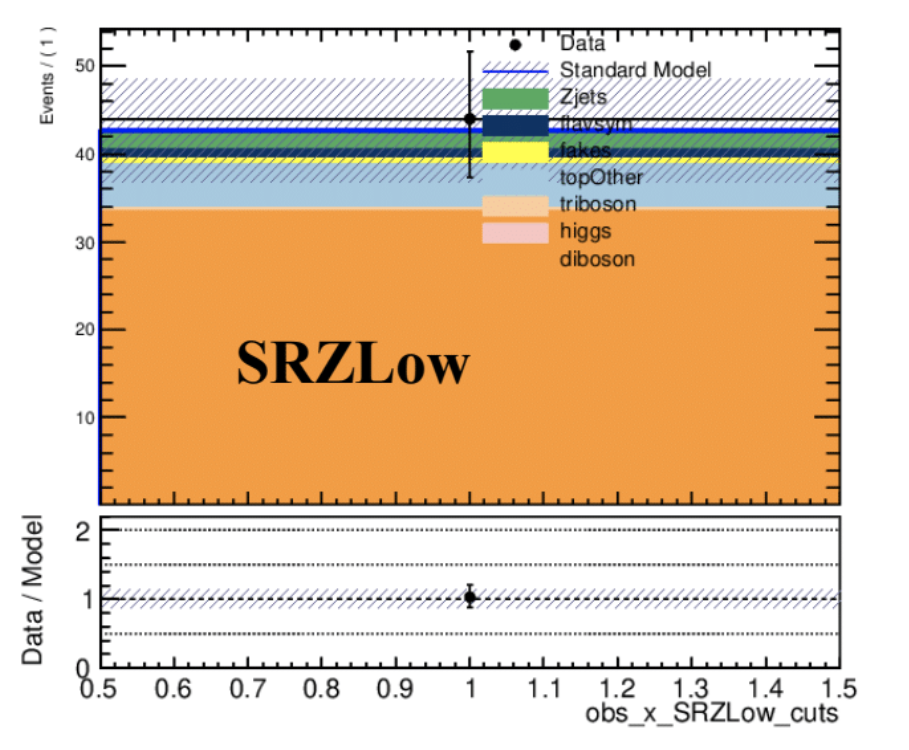
\includegraphics[width=0.45\textwidth]{Images/SUSY/on_Z_low_results.png}
    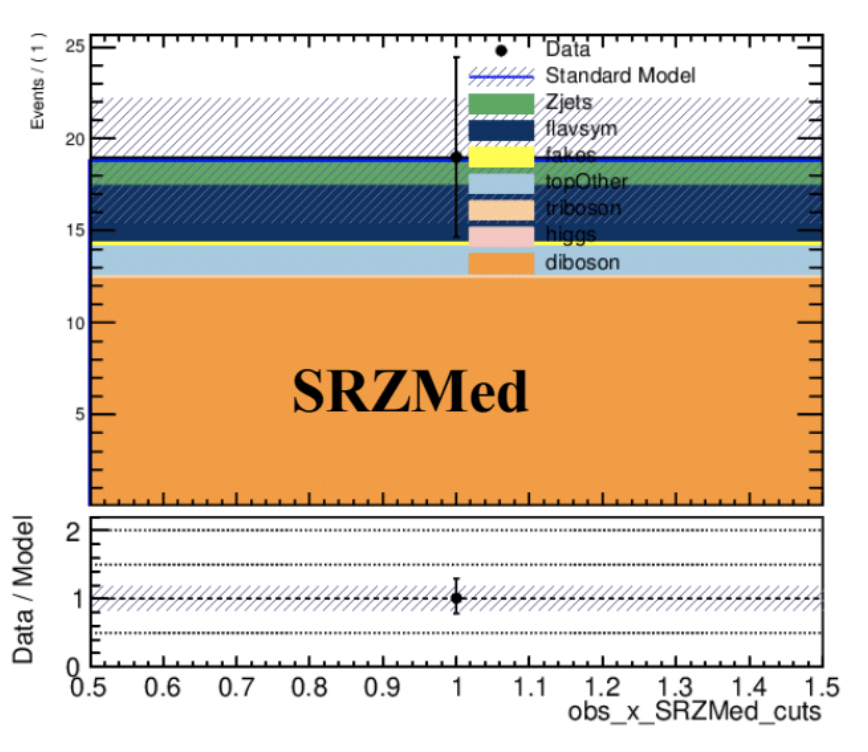
\includegraphics[width=0.45\textwidth]{Images/SUSY/on_Z_med_results.png}
    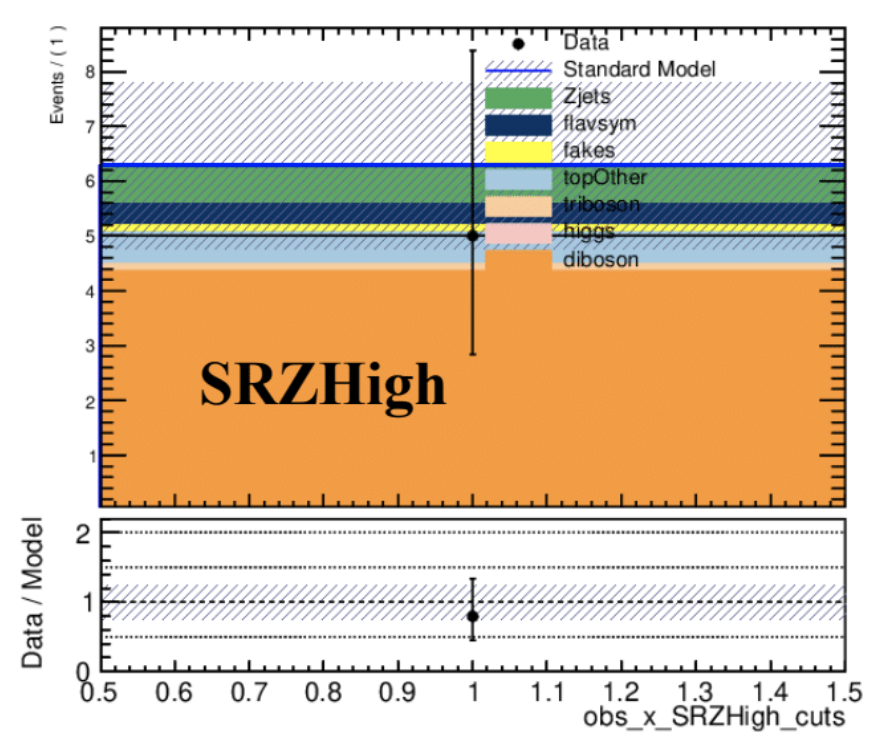
\includegraphics[width=0.45\textwidth]{Images/SUSY/on_Z_high_results.png}
    \caption{Data vs. Standard Model backgrounds for on-Z models. We see that results are within one standard deviation of expected yields.}
    \label{fig:on_Z_results}
\end{figure}

\begin{figure}[htbp]
    \centering
    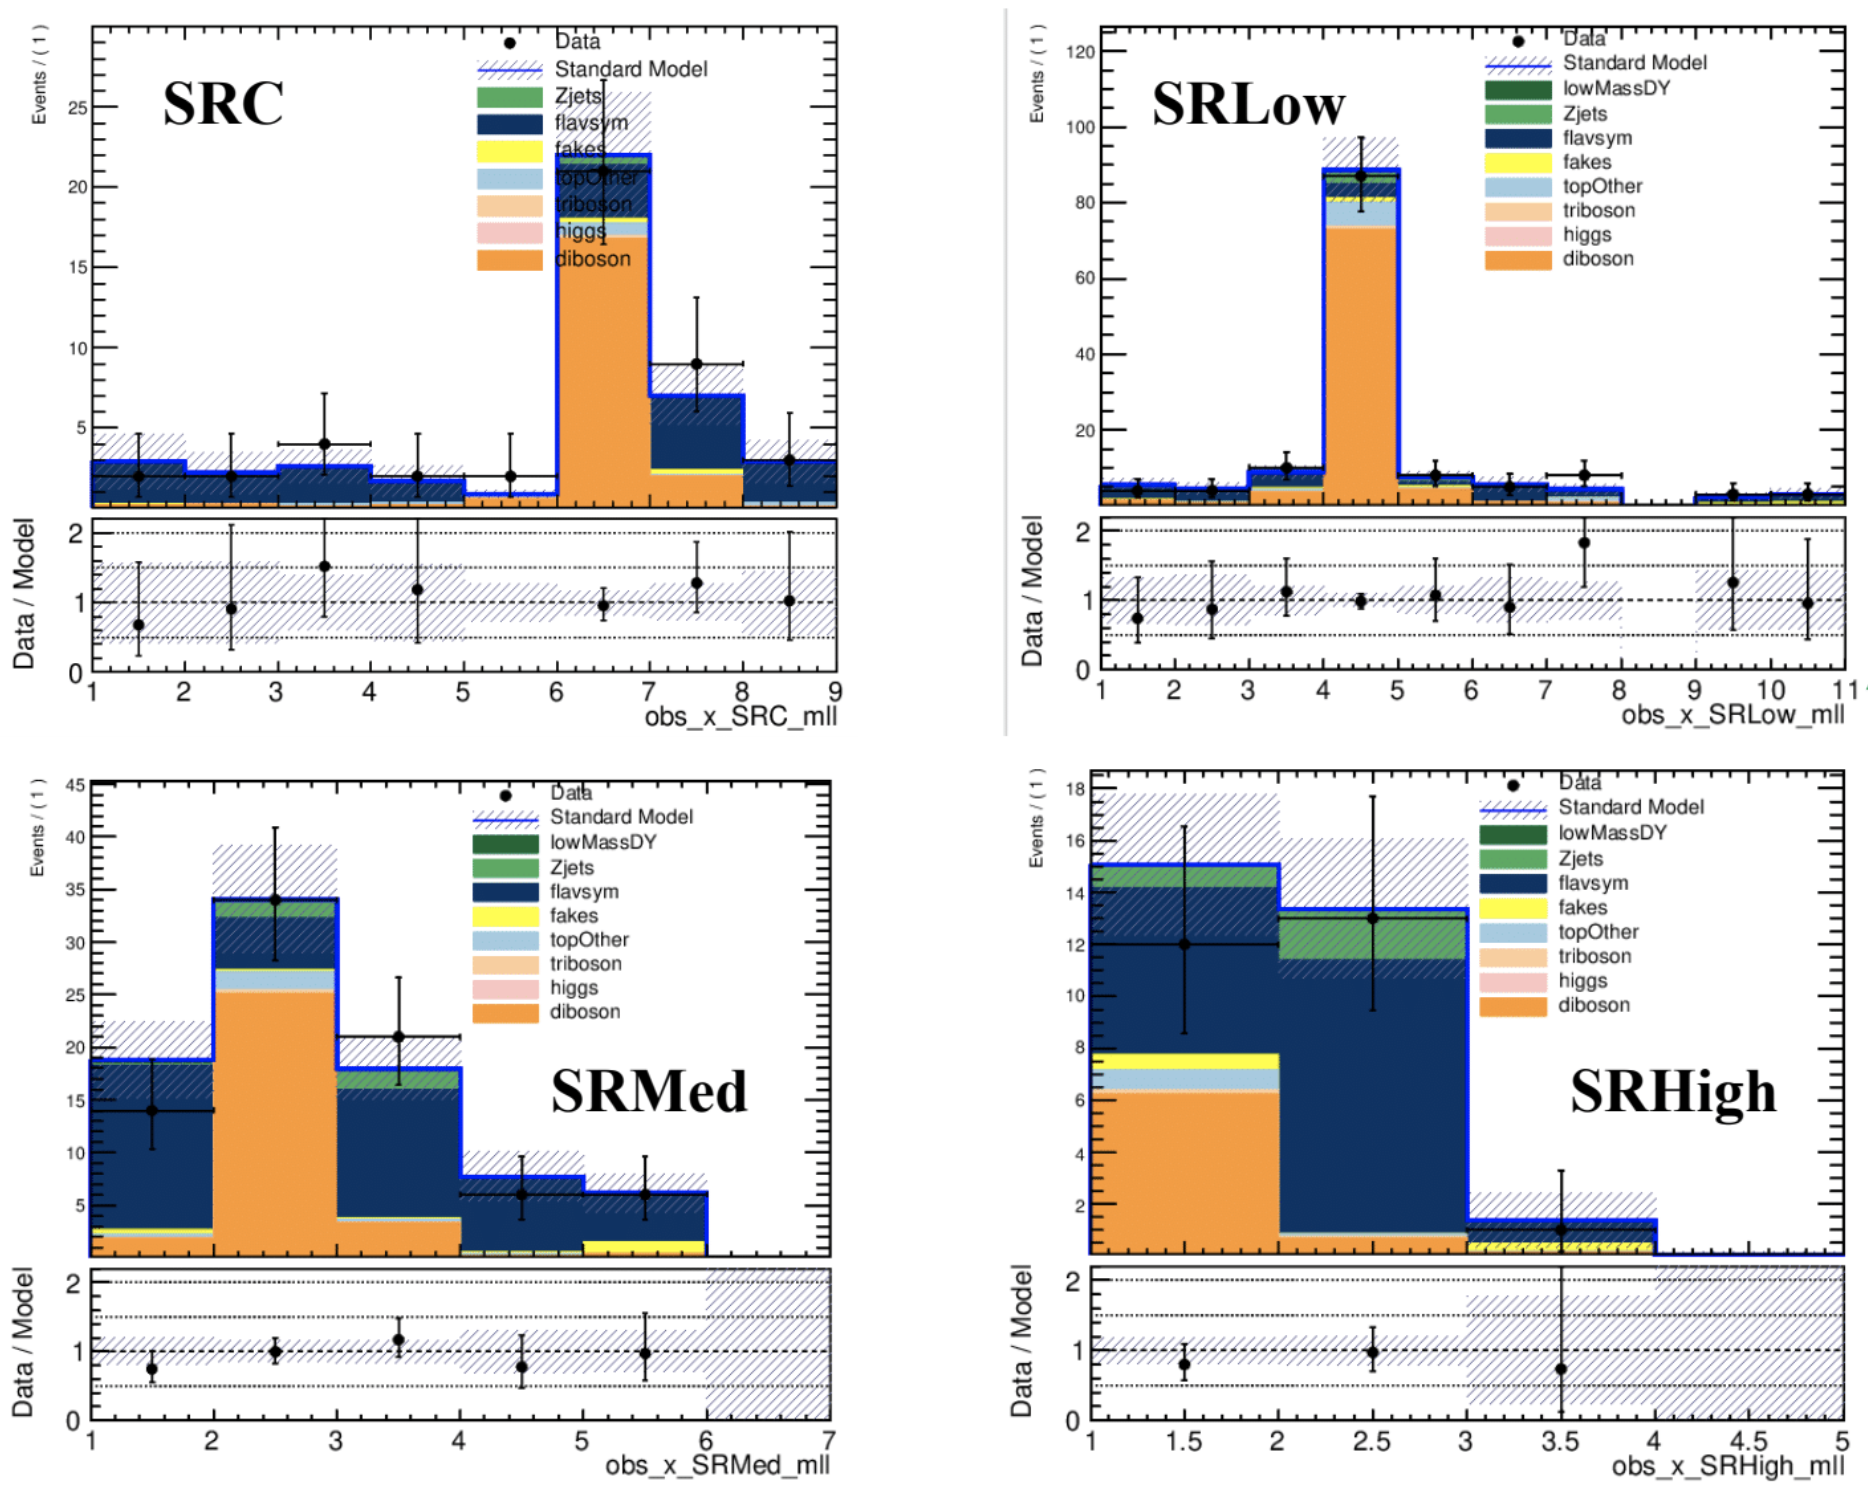
\includegraphics[width=0.85\textwidth]{Images/SUSY/edge_results.png}
    \caption{Data vs. Standard Model backgrounds for edge models. \mll\ is binned on the x axis, using bin sizes which were optimized before unblinding. We see that results are consistent with expected yields and \mll\ shapes.}
    \label{fig:edge_results}
\end{figure}

\begin{figure}[htbp]
    \centering
    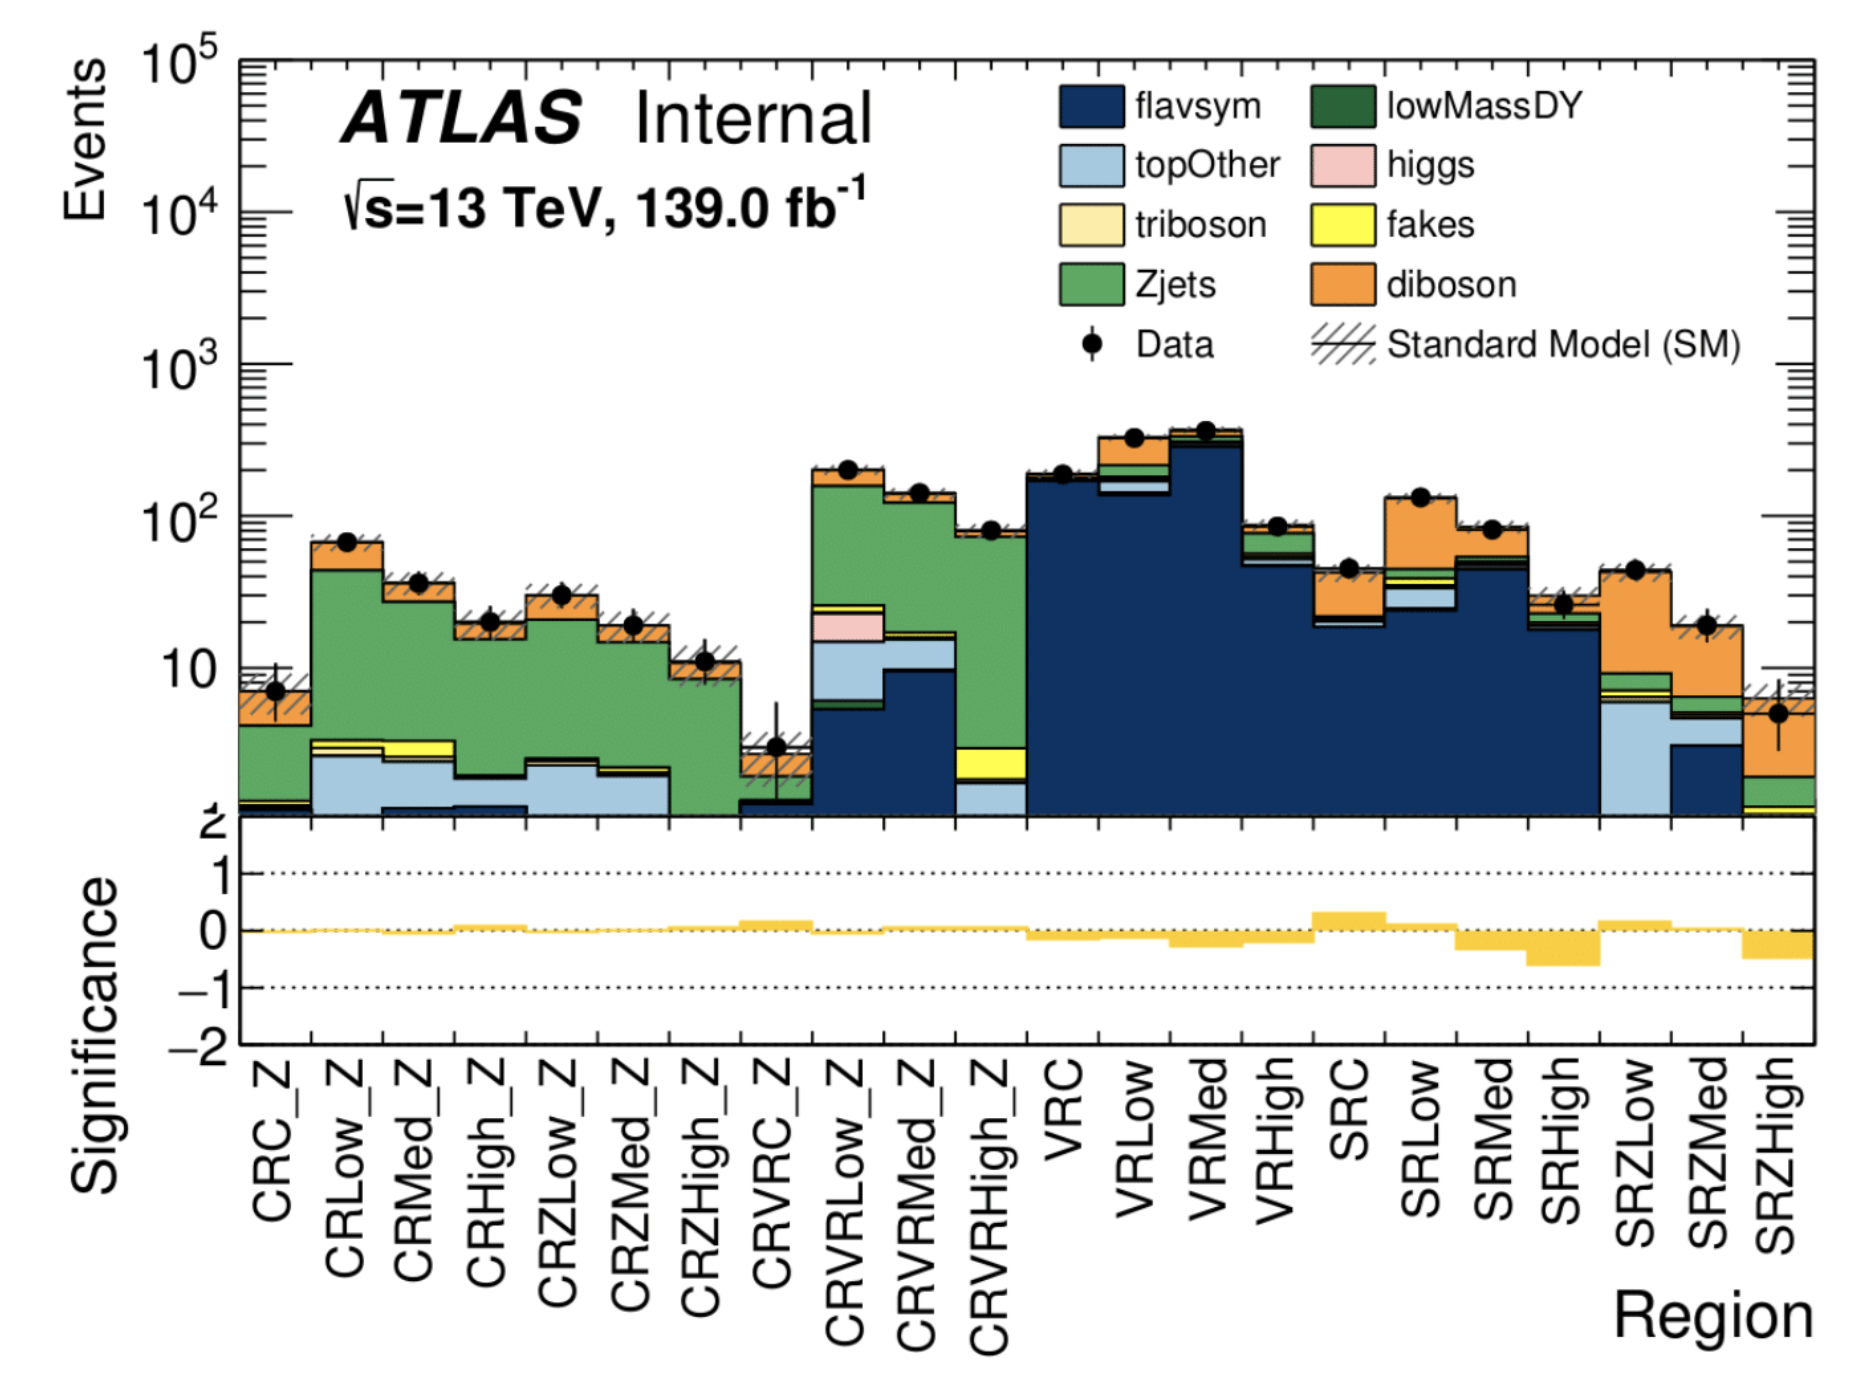
\includegraphics[width=0.85\textwidth]{Images/SUSY/all_results.png}
    \caption{A summary of data vs. Standard Model backgrounds for all regions. We see that data is within one standard deviation of expected yields in all cases.}
    \label{fig:all_results}
\end{figure} %[text/images/citations]

\part{A Brief Introduction to Machine Learning}
\chapter{How to Teach Your Machine}

Machine learning is an area of computer science in which we attempt to create intelligent systems that are able to make complex, human-level decisions. It has seen use in recent years in areas as diverse as self-driving cars, language processing, and automatic crop harvesting. In recent years, many machine learning techniques have started being applied to the realm of high-energy physics. Due to very high volumes of data production, especially for planned next-gen colliders such as the HL-LHC, and due the complexity involved in reconstructing each collision event, machine learning has increasingly been applied to tasks such as track reconstruction, vertex-finding, and jet identification, and played a part in the discovery of the Higgs. The field is extremely broad with many applications, so I will only attempt to describe a few basic ideas here.

\section{Basic Concepts}

Boiled down to its fundamentals, the goal of machine learning is to learn a function mapping. This function may map a single input (in what may be a high dimensional vector space) to a single output, as in an image classifier. It may also map multiple inputs to multiple outputs, as in the case of language translation, if we treat each word as an input or output. We may even have functions that produce a continuous stream of outputs for a continuous stream of inputs, as in a robotic system which produces actuator signals in response to its environment. Thus, the training step of machine learning may be seen as a process of function minimization, where we attempt to reduce the difference between our mapped outputs and our desired outputs.

For instance, a facial recognition system may take as its inputs a set of pixels originating from a camera or video feed, and output a pointer to a name in a database of people. A translation program may take a string of characters in one language as text input and output another string in a different language. A drone with obstacle avoidance may take input from visual systems and from mounted sensors, and output instructions to its various motors. Even an organic entity takes chemical, physical, and electrical inputs from its environment, and outputs signals to its muscles and organs, and can thus be modeled as a reinforcement learning agent.

We may classify some types of of machine learning algorithms by their training method. One type is supervised, where a system is fed a series of training examples, and is told explicitly what type of output the system should be attempting to obtain for each example. This is the case for an image classification algorithm, which may be fed many different input images, along with labels for each image. Another major class of machine learning algorithms is unsupervised learning. In this case, the algorithm is still fed input data, but is not told what the output should be. This is generally the case for clustering algorithms, such as those used for data compression and error/outlier detection. In addition, there are reinforcement learning algorithms, which process a stream of input and produce a stream of output, such as in the case of a video game playing AI. These algorithms are typically trained on a system of rewards which the algorithm gathers as it makes decisions in its environment.

Two common goals of machine learning algorithms are to perform classification and regression. In the case of classification, an algorithm is provided an input (or multiple inputs), and calculates a set of probabilities for which discrete classes the input may fall into. Image classification algorithms of course fall into this category. On the other hand, regression algorithms are used when there are not a discrete set of possible outputs. Rather, the net output is allowed to be unbounded (or at least continuous within a range), and the algorithm is graded based on how close its output gets to the target output. In some sense, language-based algorithms are typically classification-based, since there are a discrete number of words in a language to choose from. Image generation algorithms can be seen as regression-based, since we grade the generated image based on how close it is in vector space to a target output image.

\section{The Idea Behind Training}

As its name suggests, the field of machine learning is generally focused on how to get an algorithm to "learn" from input data, and as you've probably picked up from the preceding discussion, such learning is referred to as "training" the algorithm. A machine learning algorithm can take the form of a complicated expression with many tunable parameters. This expression may be in the form of a series of matrix operations, or as a chain of cut-based classifiers, or in general any other form of an input-output system with tunable components. In a supervised learning example, this algorithm begins with some initial (and probably randomized) parameters, and essentially spits out random outputs when given inputs. We train the algorithm by feeding it chunks of input data (called training data), and grading it based on comparing its outputs to the correct outputs. We tweak the parameters of the algorithm based on its performance after each training step. Once the algorithm is sufficiently trained, we can gauge the robustness of its performance on previously unseen data (referred to as test data).

The output grading step of the training process is quantified by calculating a "loss function", which is a function of the algorithm output and the correct expected output. In practice, for regression problems the loss function is often the L2 distance between the output and target output vectors. For classification problems the loss function is often cross entropy loss as shown in Equation~\ref{eq:cross_entropy}. In this equation, the sum is over all class indices $i$, $p$ is the target output distribution, and $q$ is the predicted output distribution. For example, if we are training an algorithm to recognize handwritten digits, we may have ten possible output classes (0-9). If we are then trying to recognize a handwritten digit 3, and our algorithm believes that the digit is a 2 with probability $15\%$ and a 3 with probability $85\%$, our cross entropy loss would be $-0\cdot\log(.15)-1\cdot\log(.85)$. As a concept, cross entropy measures how many bits would required on average to encode an event with a true probability distribution $p$ given an encoding scheme optimized for a probability distribution $q$. A high cross entropy indicates a large mismatch in underlying probability distributions.

\begin{equation}
\centering
H(p,q) = -\sum_{i} p_i \log q_i
\label{eq:cross_entropy}
\end{equation}

In all instances, our goal would be to tweak our algorithm such that the loss function is minimized over all training data. The specific way we do this depends on the algorithm, and we will discuss two common algorithms and their training methods in the next chapter. %[citations]
\chapter{Basic Algorithms}

I will now talk about two very common machine learning algorithms, the boosted decision tree (BDT) and the neural net. Neural nets in particular form the basis of most modern machine learning, and all advanced architectures discussed in this thesis will be some form of neural network.

\section{BDTs}

Simply speaking, a decision tree is simply a series of branching paths based on input data, which one can follow to reach a conclusion. An example of a very simple decision tree is shown in Figure~\ref{decision_tree}. Decision trees are similar to how objects and signal regions are selected in a traditional high-energy-physics analysis. For example, one may ask whether an event has more than, less than, or equal to three leptons. If the event has exactly three leptons, one may ask whether the top two leptons have dilepton mass within a certain range, etc. Based on these decisions, an experimenter can decide what signal region an event belongs in. As another example, imagine that we are trying to determine what kind of particle we have seen in an event. We could ask whether the particle left a track in the inner detector, whether the amount of energy it deposited in the calorimeter is in a certain range, etc. Given a random ordered set of input variables, an optimal decision tree can be calculated for decisions made in that specific order.

A boosted decision tree is created by combining many different decision trees together \cite{BDT}. Any given decision tree can be very weak, containing only a small number of branches and a small maximum depth. However, by taking the weighted results of many decision trees together, we can get a more accurate result than can be achieved by any single tree. For the sake of space, the AdaBoost BDT training algorithm will not be discussed here.

\begin{figure}[t]
    \centering
    %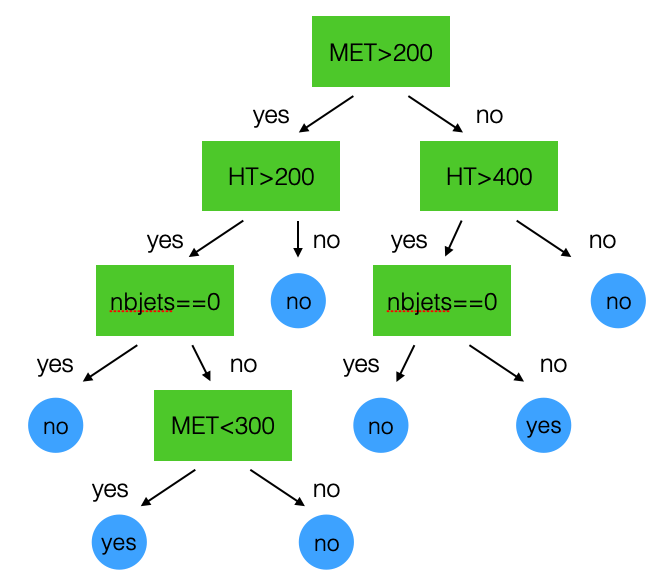
\includegraphics[width=0.5\linewidth]{images/decision_tree.png}
    \caption{An example of a decision tree that a child may use to classify a household pet.}
    \label{decision_tree}
\end{figure}

\section{Neural Nets}

A neural net is a machine learning architecture based on the physical structure of neurons in the human brain \cite{neural_net}. The basic unit of a neural net is a neuron, which has a numerical value, one or more inputs, and one or more outputs. These neurons are connected together so that the output of one neuron becomes the input of one or more other neurons. Here we will only consider simple feed-forward neural nets, where all the inputs to a neuron come from neurons closer to the beginning of the net, and all the outputs of that neuron go to neurons nearer the end of the net. That is, there are no "loops", and there are no connections between neurons at the same depth. The input values for an event form the first layer of neurons, and the output is derived from the last layer. Each link between neurons is associated with a "weight", or multiplicative constant. Each neuron is also associated with a "bias", or an additive constant. Letting $y_i$ be the value of the $i^{th}$ neuron, $w_{i,j}$ be the value of the weight between neurons $i$ and $j$, and $b_i$ be the bias associated with neuron $i$, we see that the value of a neuron is equal to $y_j = \sum{w_{i,j}y_i} + b_j$. Each neuron is also typically followed by a nonlinear "activation" function, so that the result of the entire net is not simply equivalent to a single matrix operation on the input. We see then that for a given set of weights and biases, we can calculate the output value for a net given any inputs.

In order to train a neural net, we use "back-propagation", meaning that for each event (or set of events) we perform gradient descent on each weight and bias in order to minimize the resulting loss function. Over the course of many events, the net can fall into a state where it produces the correct outputs with high accuracy. In this way, the neural net training is simply a form of function optimization. Many important topics, such as how to weight initialization, methods of gradient descent, net architectures, etc. will not be discussed in this paper.

\begin{figure}[t]
    \centering
    %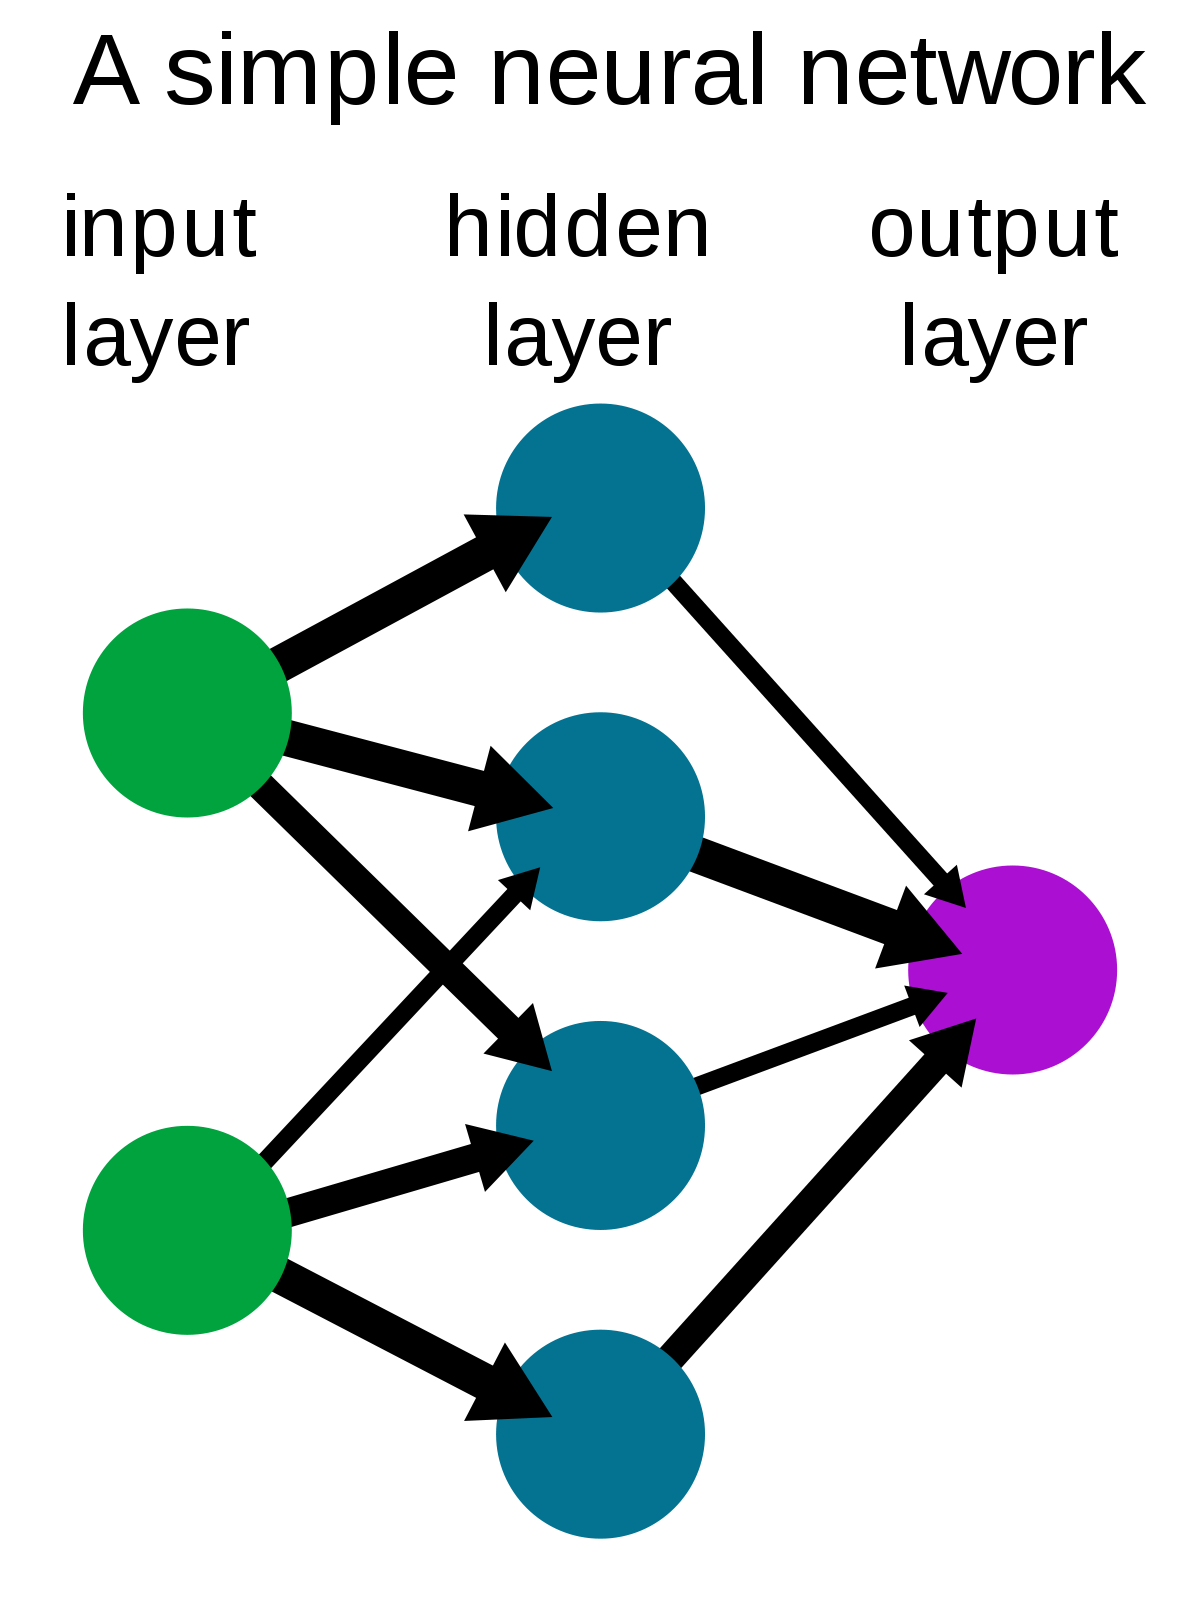
\includegraphics[width=0.5\linewidth]{images/neural_net.png}
    \caption{A diagram showing a typical densely-connected neural net.}
    \label{neural_net}
\end{figure} %[citations]
\chapter{Advanced Architectures}\label{sec:advanced_architectures}

\section{Convolutional Nets}

\section{GoogLeNet}

\section{Autoencoders}

An autoencoder, shown in Figure~\ref{fig:autoencoder}, is an architecture which has the same number of neurons in its input and output layers, but which contains at least one hidden layer which has fewer neurons. These nets are trained in a semi-unsupervised manner, by simply trying to get the outputs to replicate the inputs. If we take $\hat{x}$ to be the input vector and $\hat{y}$ to be the output vector, a simple loss function for training an autoencoder is:

\begin{align}
    \mathcal{L} &= (\hat{y}-\hat{x})^2
\end{align}

\begin{figure}[htbp]
    \centering
    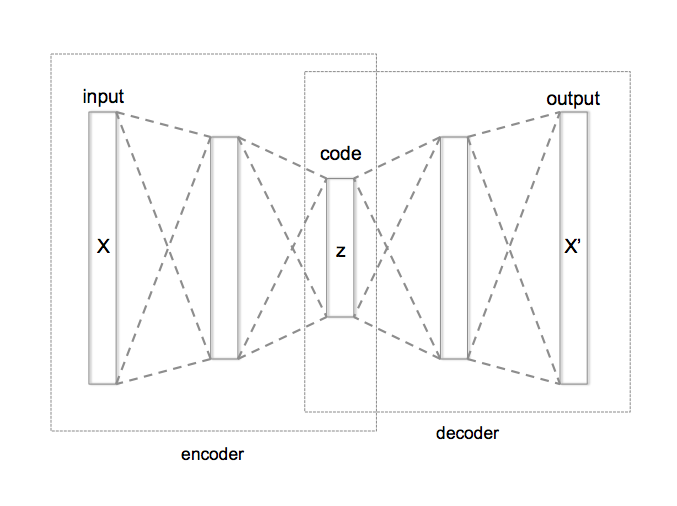
\includegraphics[width=\linewidth]{Images/ML/autoencoder.png}
    \caption{Autoencoder architecture, from~\cite{autoencoderDiagram}.}
    \label{fig:autoencoder}
\end{figure}

The purpose of an autoencoder is to perform dimensionality reduction. In Figure~\ref{fig:autoencoder}, our net has learned a compressed encoding of its data space, as represented by the neurons on the $\hat{z}$ layer. The trained structure can then be used for many purposes, such as for data compression or for image generation with generative adversarial nets.

The layers of the autoencoder may be simply connected, or they can be more complex structures, such as convolutional layers.

\section{Generative Adversarial Nets}

A generative adversarial network (GAN) can be used to create simulated samples in some data space. A GAN can be used to generate images, speech, video, or any other kind of data. Two famous examples of this type of network are StyleGAN, which can be used to generate faces and other images, and Google DeepDream, which can be used to generate surreal pictures and videos.

In a GAN we have two nets, the generator and the discriminator, competing against each other. To explain the process we will consider the case of a GAN which can generate images of a requested class.

The generator begins as the decoder half of a trained autoencoder, as seen in Figure~\ref{fig:autoencoder}. This autoencoder has been trained not only to replicate input data, but also to perform classification on it, as represented by a subset of the neurons on the $\hat{z}$ layer. Thus, layer $\hat{z}$ is a compressed representation of the image space, with a subset of neurons indicating image class and the rest of the neurons representing other salient features about the image.

In order to generate a new image with the generator, we feed to layer $\hat{z}$ the desired classification, along with a vector of randomized noise for the other neurons. Propagating through the generator creates an output of the desired class.

The discriminator half of the network is a trained classifier which is able to determine the class of an image. We tweak this architecture by adding an output which also classifies the image as "real" or "generated".

This is where the "adversarial" part of a GAN comes into play. The two nets are now trained against each other. First we request an image of a random class from the generator, and feed that image to the discriminator. The generator loss function is based on the image classification accuracy of the discriminator and on whether or not the discriminator was fooled into thinking the image was real. Next we train the discriminator by feeding it a mix of real and generated images, and grading it by discrimination accuracy. This process is repeated back and forth until convergence.

\section{Recurrent Neural Nets}

Up until now we have described typical feedforward neural nets, where connections between nodes go from layer to layer and do not loop back to previous layers. We will now describe a class of recurrent architectures which do not exhibit this behavior. Rather, as seen in Figure~\ref{fig:RNN}, a recurrent neural net (RNN) has a set of "hidden" neurons which loop from the output layer back to the input layer. We can use these kinds of nets for processing time series or sequential data by feeding the data sequence (e.g. a string of words that form a sentence) into the net one piece at a time. We begin with a randomly initialized hidden state. After each piece of input passes through the net, we get an output and an updated hidden state. The hidden state is brought back around to the beginning of the net, and is fed back in along with the next piece of sequential data. In this way the hidden neurons are able to act as a sort of memory state, and to encode some sort of ongoing information about the sequence. A recurrent net can turn a sequence of inputs into a sequence of outputs, but in many situations we only care about the final output, which may be used for classification.

\begin{figure}[htbp]
    \centering
    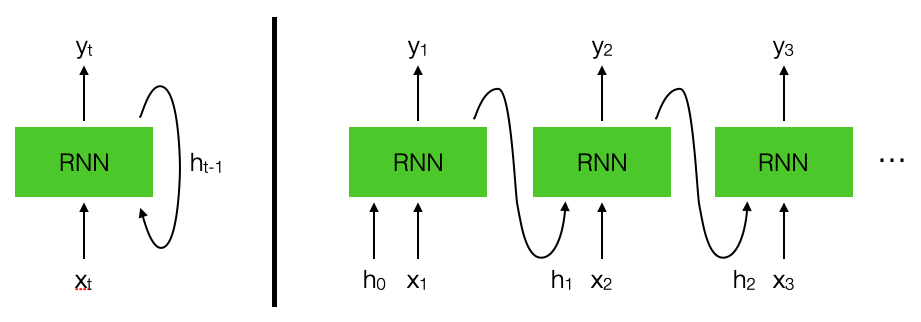
\includegraphics[width=\linewidth]{Images/ML/RNN.png}
    \caption{A standard recurrent neural net, shown in condensed form on the left, and in expanded form on the right. This net takes inputs $x_i$ and provides outputs $y_i$. A hidden state $h_i$ is retained in the net and passed back to the beginning after each input step.}
    \label{fig:RNN}
\end{figure}

The actual body of the RNN can be a neural net of any architecture, but in a standard RNN we typically use a simple few-layer densely connected net. The hidden state and output also typically pass through a $\tanh$ layer, with the output passing through an additional softmax layer. In this case, if we write the concatenation of $x_t$ and $h_{t-1}$ as $x_t \oplus h_{t-1}$ and the neural net weight matrix as $W$, we can represent the RNN via the following equations:

\begin{align}
    o_t\oplus h_t&=\tanh(W(x_t\oplus h_{t-1})) \\
    y_t&=\text{softmax}(o_t)
\end{align}

If we examine this equation, we can see a problem which commonly comes up when training an RNN via gradient descent. We see that the final output $y_n$ depends on $W$, $x_n$, and $h_{n-1}$. But then $h_{n-1}$ further depends on $x_{n-1}$ and $h_{n-2}$, and so on. If we work out the full derivative of $y_n$ with respect to $W$, we get the following:

\begin{align}
    \frac{dy_n}{dW}&=\frac{\partial y_n}{\partial W} + \frac{\partial y_n}{\partial h_{n-1}}\frac{dh_{n-1}}{dW} \\
    &=\frac{\partial y_n}{\partial W} + \frac{\partial y_n}{\partial h_{n-1}}[\frac{\partial h_{n-1}}{\partial W} + \frac{\partial h_{n-1}}{\partial h_{n-2}}\frac{dh_{n-2}}{dW}] \\
    &=\frac{\partial y_n}{\partial W} + \frac{\partial y_n}{\partial h_{n-1}}[\frac{\partial h_{n-1}}{\partial W} + \frac{\partial h_{n-1}}{\partial h_{n-2}}[
    \frac{\partial h_{n-2}}{\partial W} + \frac{\partial h_{n-2}}{\partial h_{n-3}}\frac{dh_{n-3}}{dW}
    ]] \\
    &=... \nonumber
\end{align}

We then see that for all $t$:

\begin{align}
    \frac{\partial h_t}{\partial h_{t-1}} &= \tanh'(W(x_t\oplus h_{t-1}))W \\
    \frac{\partial h_t}{\partial W} &= \tanh'(W(x_t\oplus h_{t-1}))(x_t\oplus h_{t-1}) \\
    \frac{dy_n}{dW} &\approx \sum_{t=1}^{n} [\tanh'(W(x_t\oplus h_{t-1}))]^{n+1-t}W^{n-t}(x_t\oplus h_{t-1})
\end{align}

The powers of $W$ and the powers of the derivative of $\tanh(x)$ are both problematic here, since they quickly approach zero, causing terms with low values of $t$ to essentially become irrelevant to training. In other words, the basic RNN has trouble learning long-range dependencies, and will in a sense "forget" the beginning of a sequence by the time it has calculated the final output. This behavior is called the vanishing gradient problem. In the case that W is large enough, we have the exploding gradient problem instead, but this issue is less common and is easily fixed by clipping gradients at a set maximum.

\section{LSTM and GRU}

One method of dealing with the vanishing gradient problem is the use of long short-term memory (LSTM) nets, first proposed in 1997. This type of net, shown in Figure~\ref{fig:LSTM_diagram}, has an internal structure in each recurrent cell which is more complex than a simple neural net. Each cell contains a forget gate, an input gate, and an output gate, which determine how much the cell state should update to accommodate new information, and how much information it should output. We have two internal states in an LSTM, $c_t$ and $h_t$. $c_t$ is similar to the hidden cell state in the basic RNN, and $h_t$ acts as the cell output at each step, but is also carried over to the input of the next step.

\begin{figure}[htbp]
    \centering
    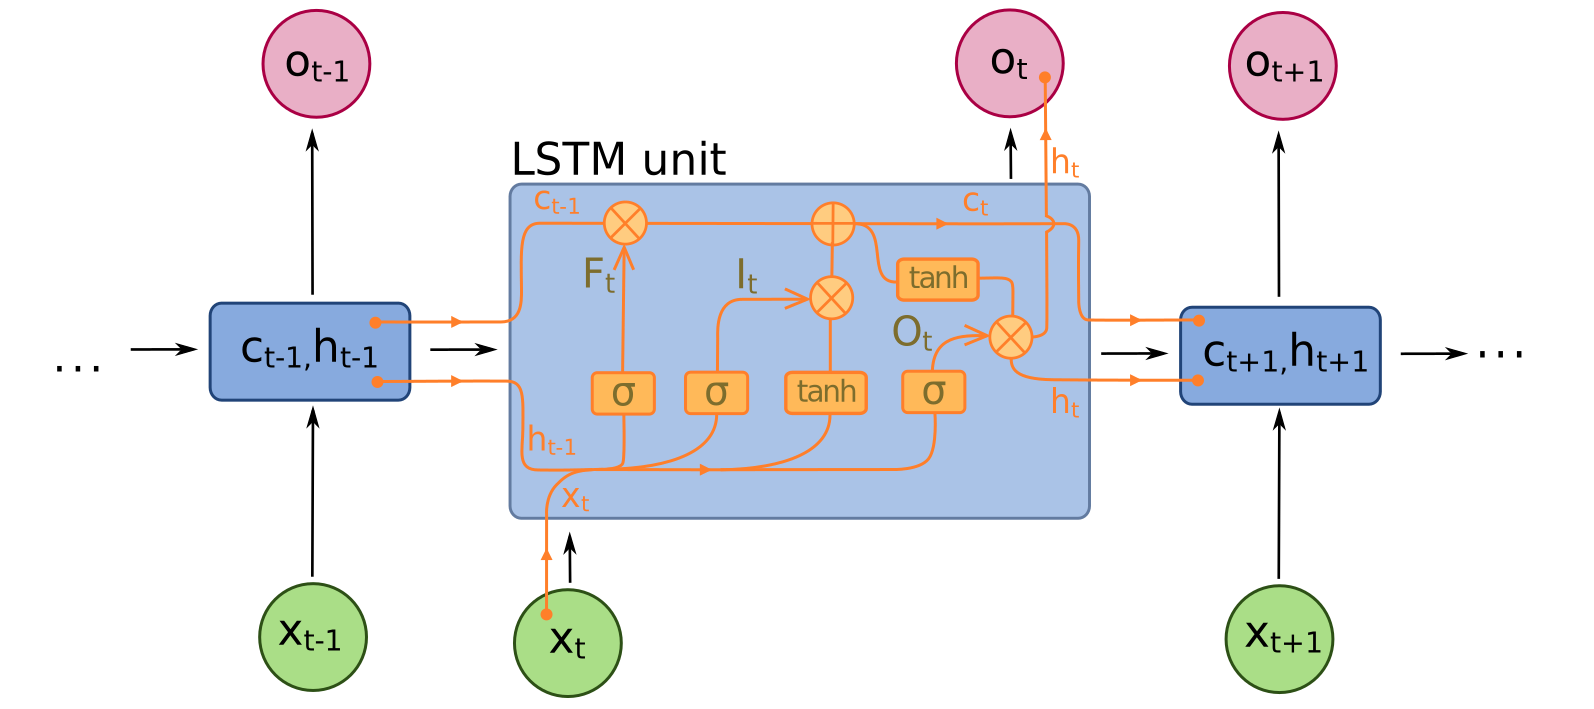
\includegraphics[width=\linewidth]{Images/ML/LSTM.png}
    \caption{LSTM architecture, showing the forget gate ($F_t$), input gate ($I_t$), and output gate ($O_t$) present in each cell. Taken from~\cite{LSTMDiagram}.}
    \label{fig:LSTM_diagram}
\end{figure}

The LSTM works as follows. At each time step $t$, we feed the input $x_t$, the previous output $h_{t-1}$, and the previous cell state $c_{t-1}$ into the net. $x_t$ and $h_{t-1}$ are used to determine the forget factor $F_t$, the input factor $I_t$, and the output factor $O_t$, all of which are vectors with components that lie between 0 and 1. The forget factor is multiplied onto $c_{t-1}$, allowing the cell to "forget" some of its previous state. The input factor is used to determine how much of the current input then gets added to the cell state. Finally, the output factor is multiplied by the new cell state to give $h_t$, the cell output. All together, the equations for an LSTM are as follows:

\begin{align}
    F_t &= \sigma(W_f (x_t \oplus h_{t-1})) \\
    I_t &= \sigma(W_i (x_t \oplus h_{t-1})) \\
    c_t &= c_{t-1} \cdot F_t + I_t \cdot\tanh(W_c (x_t \oplus h_{t-1})) \\
    O_t &= \sigma(W_o (x_t \oplus h_{t-1})) \\
    h_t &= O_t \cdot\tanh(W_h c_t)
\end{align}

The derivation is beyond the scope of this overview, but the gradient of the loss in this case will not have an exponential dependence on any weight matrix $W$, nor on the derivative of the sigmoid or tanh. Essentially, the $c_t$ state ensures that all inputs have non-zero contribution to the loss term. Thus, the LSTM is much less prone to the vanishing gradient problem.

The gated recurrent unit (GRU) net, introduced in 2014 and shown in Figure~\ref{fig:GRU_diagram}, further improves on the LSTM by reducing its complexity while maintaining its avoidance of the vanishing gradient problem. A GRU only has two gates, an update gate and a reset gate. In this architecture the reset gate controls how much information from the hidden state gets added to the input. The update gate conversely controls how much input information gets mixed back into the hidden state. The hidden state $h_t$ also acts as the output at each step, making the structure of the GRU somewhat less effective for multi-output data.

\begin{figure}[htbp]
    \centering
    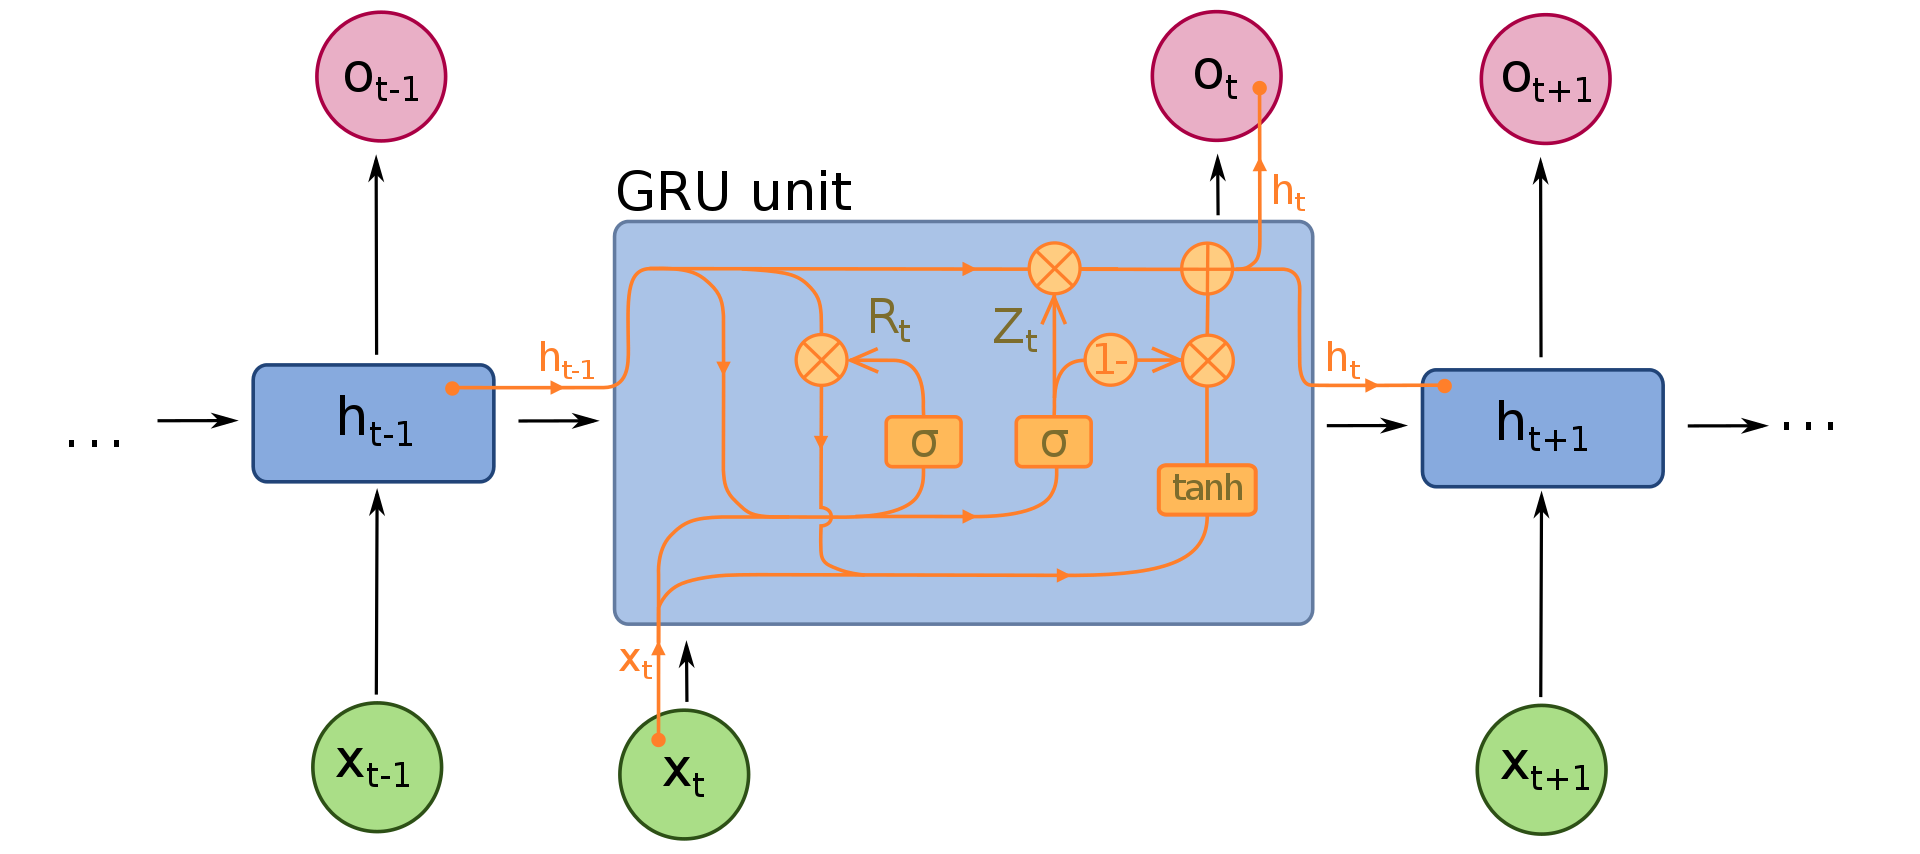
\includegraphics[width=\linewidth]{Images/ML/GRU.png}
    \caption{GRU architecture, showing the update gate ($Z_t$) and reset gate ($R_t$) present in each cell. Taken from~\cite{GRUDiagram}.}
    \label{fig:GRU_diagram}
\end{figure}

\begin{align}
    R_t &= \sigma(W_r (x_t \oplus h_{t-1})) \\
    Z_t &= \sigma(W_z (x_t \oplus h_{t-1})) \\
    h_t &= Z_t h_{t-1} + (1-Z_t)\tanh(R_t h_{t-1} + x_t)
\end{align}

\section{Seq2Seq}

A seq2seq architecture consists of an encoder recurrent net and a decoder recurrent net, as seen in Figure~\ref{fig:seq2seq}. This type of net takes an input sequence and processes it with the encoder. This processed vector, which contains information about the entire sequence, is then passed to the decoder and used to output a different sequence, not necessarily of the same length as the input.

\begin{figure}[htbp]
    \centering
    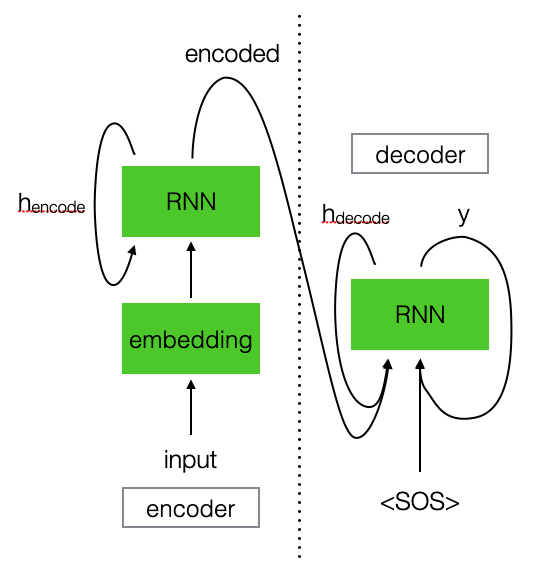
\includegraphics[width=0.55\linewidth]{Images/ML/seq2seq.png}
    \caption{Seq2Seq architecture. The encoder takes words in a sentence, embeds them in a word vector space, and passes the embedded vectors into an RNN. The final output of the encoder is sent to the decoder as its initial hidden state. The decoder begins with SOS as its initial input, and loops until it outputs EOS. The entire decoder sequence is the output sentence.}
    \label{fig:seq2seq}
\end{figure}

Seq2Seq is commonly used for language translation, so inputs in these cases are first transformed into a "word vector" in some embedding space before they go through the encoder. Describing word embeddings is outside the scope of this review, but the idea is that similar words are close together in this vector space, and pairs of words with the same relations have similar vector differences. In other words, the embedding captures some semantic structure between words. Common embeddings include word2vec and GloVe.

In more detail, the encoder takes a sequence of inputs $\hat{x}$ and runs it through an RNN to produce a sequence of outputs $\hat{s}$. In a simple seq2seq architecture, we take only the final output, which we denote as $s$, to pass to the decoder. The decoder takes $s$ as an initial hidden state, and the start-of-string (SOS) signal as an initial input, and performs a typical recurrent architecture loop to generate an output sequence. The sequence ends when the decoder outputs an end-of-string (EOS) signal.

A seq2seq architecture may also include an attention mechanism, as shown in Figure~\ref{fig:seq2seq_with_attention}. In this case the decoder has an additional step where it uses its input and hidden state to obtain an attention vector. We take the dot product of this attention vector with the entire encoder output sequence $\hat{s}$ to get a sort of weighted vector. Essentially, the attention vector allows us to focus on different parts of the input sequence as we're producing the output.

Details about the training of seq2seq are outside the scope of this review.

\begin{figure}[htbp]
    \centering
    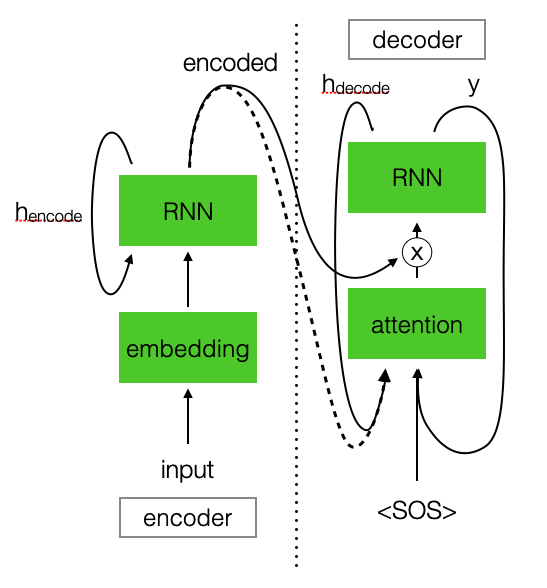
\includegraphics[width=0.55\linewidth]{Images/ML/seq2seq_with_attention.png}
    \caption{Seq2Seq architecture with an attention mechanism added. Now the entire encoder output is used by the decoder. The final output of the encoder is still used as the decoder's initial hidden state, but now the hidden state and decoder input are used to calculate an attention vector, which passes through a softmax layer to add up to 1. The dot product of this attention vector with the entire encoder output sequence then produces a weighted encoder output which is sent to the decoder RNN.}
    \label{fig:seq2seq_with_attention}
\end{figure}

\section{Transformers}

Transformers build on the idea of using attention, but take the concept further by removing the recurrent neural net from the encoder altogether and relying solely on attention to encode positional and relational information~\cite{transformer}. The transformer thus relies on attention to figure out which parts of the input are important for the decoder at each step of the output.

The transformer architecture is shown in Figure~\ref{fig:transformer}. Once again the input is embedded in some word space before being fed to the encoder. However, now we also add an additional positional encoding vector onto each word to represent its location in the input sequence, to make up for the lack of an RNN. A detailed description of the positional encoding is beyond the scope of this review. The encoder itself is then made up of a series of sequential modules each composed of a multi-head attention mechanism (described below) and a feedforward net. A skip connection is used to add the input of each sublayer to its output.

\begin{figure}[htbp]
    \centering
    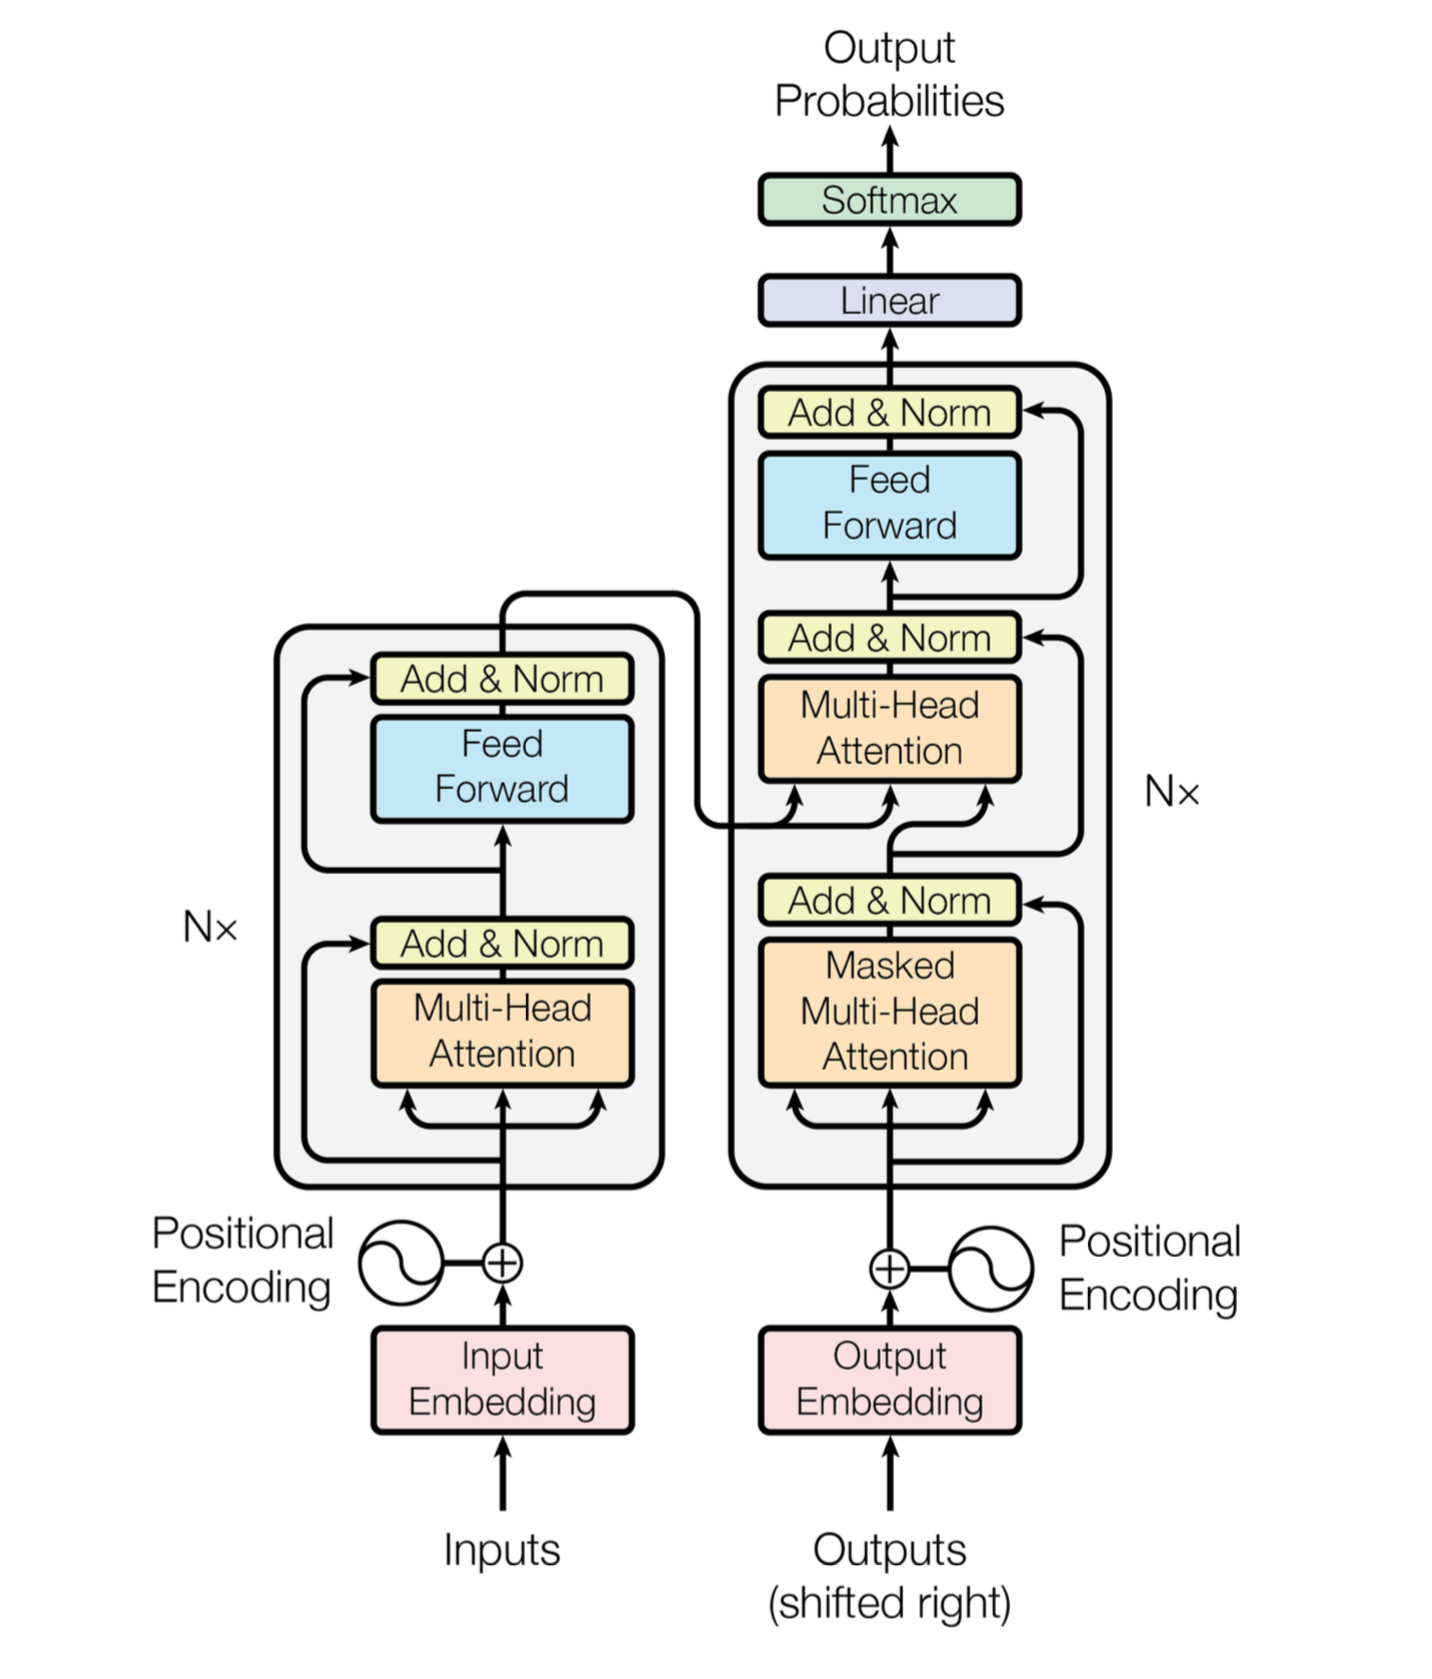
\includegraphics[width=0.7\linewidth]{Images/ML/transformer.png}
    \caption{Transformer architecture. Taken from~\cite{transformer}.}
    \label{fig:transformer}
\end{figure}

The multi-head attention mechanism in shown in Figure~\ref{fig:transformer_dot_product_attention}. Here, $Q$, $K$, and $V$ stand for query, key, and value. The $Q$ and $K$ vectors are used as in a content retrieval system, where the dot product of two vectors indicates their similarity. $V$ is the representation of a word in whatever relevant space we're using, and may or may not be equivalent to $K$. $Q$ and $K$ are of dimension $d_k$, and $V$ is of dimension $d_v$. In the simplest example, the vector embeddings of the input words are used for $Q$, $K$, and $V$, with all three matrices being equivalent. Using each word in an input this way to calculate an attention vector for the other words in the input is a concept called self-attention. The total self-attention matrix is then calculated as follows, where we have used a scaling factor to normalize the matrix product:

\begin{align}
    Attention(Q,K,V)&=\text{softmax}(\frac{QK^T}{\sqrt{d_k}})V
\end{align}

\begin{figure}[htbp]
    \centering
    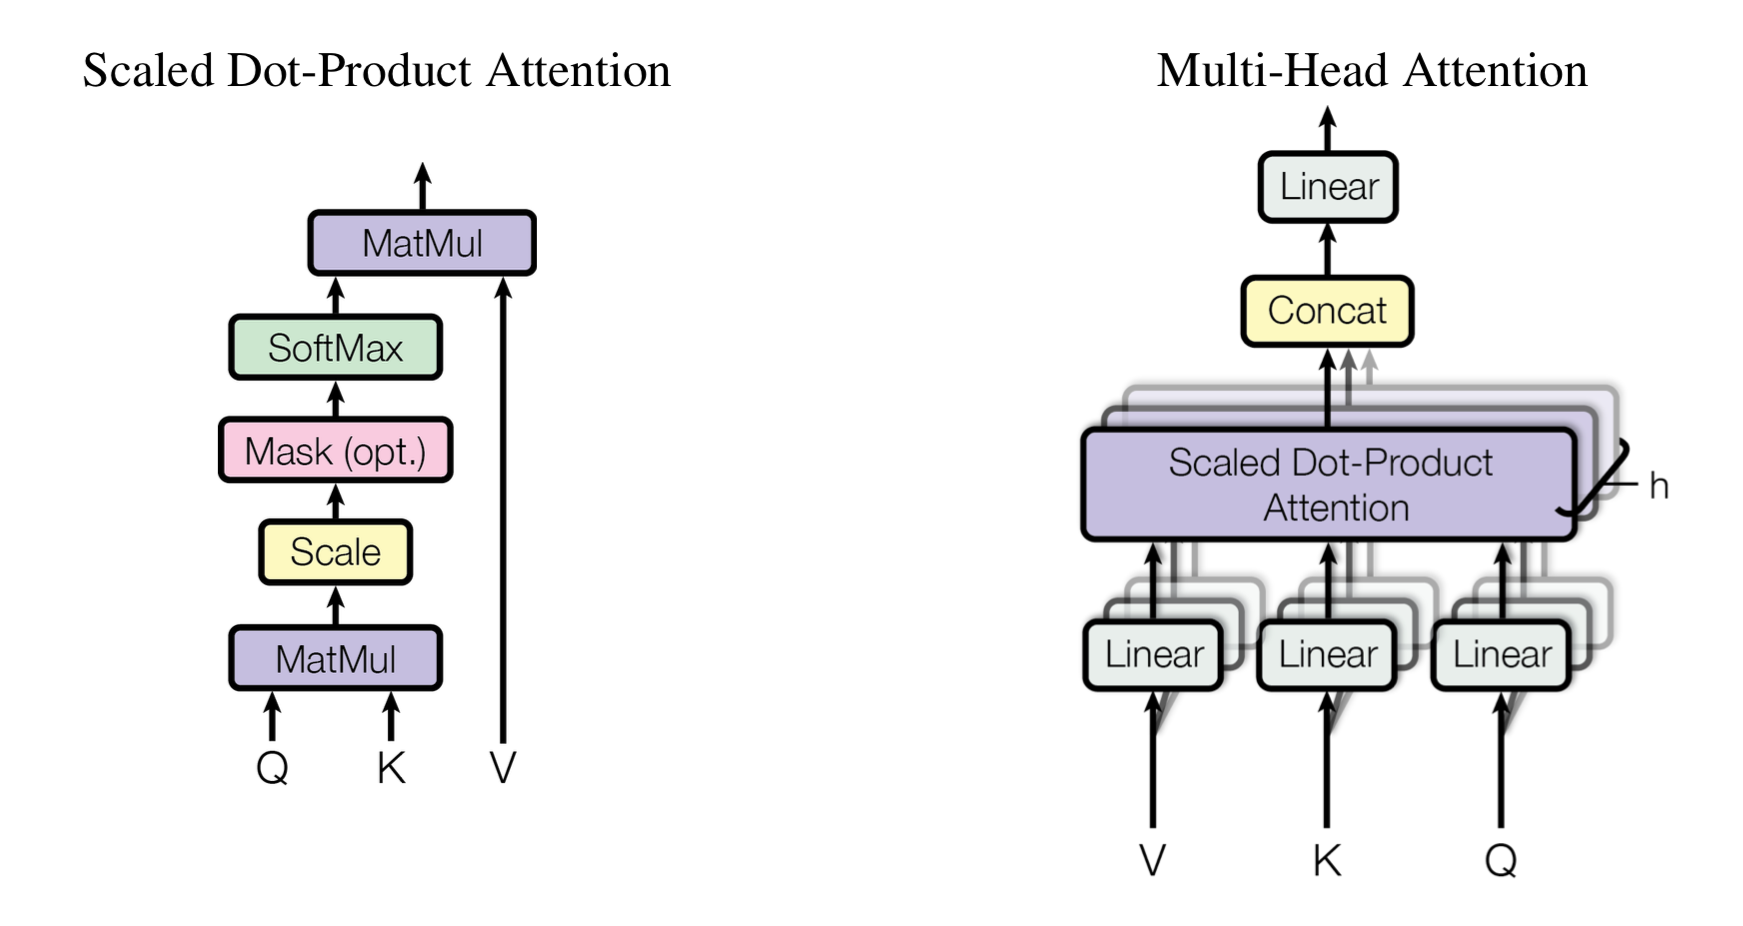
\includegraphics[width=\linewidth]{Images/ML/transformer_dot_product_attention.png}
    \caption{Mutli-head self attention mechanism. Taken from~\cite{transformer}.}
    \label{fig:transformer_dot_product_attention}
\end{figure}

In a more general multi-head attention mechanism, we don't simply use the word vector embeddings for $Q$, $K$, and $V$. Rather, we learn $h$ different sets of vectors $v_Q$, $v_K$, and $v_V$, which we project our word embeddings upon in order to obtain $h$ sets of $Q$, $K$, and $V$. The end result is that we get $h$ sets of attention matrices, where each attention matrix is some attention-weighted encoding of the relevant self-context for each input word. The $h$ matrices are then concatenated and sent through a linear layer to provide a single input-sequence encoding.

The decoder uses the same multi-headed attention idea, but the attention layer is masked, so that during training the decoder can only see words which have been outputted so far, rather than the entire output sequence. There is also a second multi-headed attention layer, which uses the output of the encoder for the keys and values.

\section{Deep Sets}

\section {Set Transformers} %[citations]

\part{Calorimeter Shower Reconstruction and Generation Using Neural Nets}
\chapter{Problem Overview}

\section{Background}

We have seen that calorimeters are key components of particle detectors, capturing important information about particle energy and type, and we have seen that one of the first steps of any high-energy physics analysis is to use these raw calorimeter recordings along with other information from the detector to reconstruct our initial physics objects.

Particle reconstruction has traditionally relied on calculating features such as shower width and rate of energy loss, and then using these features in cut-based analyses. Here we try to apply some image-based ML techniques instead. To approach this problem, we can take a snapshot of a calorimeter deposition pattern, and treat it as a voxelized image. This image could form the input layer of a neural net, with important information about the particle then spit out on the last layer.

Using neural nets with calorimeter cell-level information would allow us to more accurately determine particle type and energy compared to traditional feature-based techniques. We can even use this technology to produce simulated calorimeter showers, as we will discuss later.

These problems are already interesting for the ATLAS and CMS detectors, but will become even more so in the future with upgrades like the HL-LHC. These next-generation detectors will improve physicists' ability to identify and measure particles by using calorimeters with much finer 3D cell arrays, such as the ones proposed for the ILC~\cite{ILC} and CLIC~\cite{CLIC} linear collider detectors, and the planned-upgrade CMS~\cite{CMSCollaboration:2015zni} detectors. Our studies presented in this thesis were done on simulated data from the CLIC detector, though we showed that the algorithms we trained were applicable to ATLAS and CMS detector geometries.

\section{The Problems}
\label{sec:problems}

Now we introduce two benchmark tasks that we aim to solve with ML algorithms: 
\begin{itemize}
    \item Particle reconstruction: starting from raw detector hits, determine the type of the showered particle and its momentum.
    \item Particle simulation: starting from generator-level information about a particle, generate a realistic detector response to a shower produced by that particle.
\end{itemize}

Our goal, of course, is to build algorithms that can beat traditional algorithms, in classification and energy regression accuracy, and in time required to generate a realistic shower image.

The work presented here extends upon previous ML investigations, including prior classification studies on ATLAS calorimeter data~\cite{Nachman_DNN} and work involving the generation of electron showers at ATLAS~\cite{Nachman_GAN,Nachman_GAN2}. Since the CLIC calorimeters used for our studies are much more granular than those in ATLAS, we were able to examine more complex models in these studies. Furthermore, we combined multiple techniques together to form a single tool which performs multiple aspects of particle reconstruction simultaneously, simply starting from a calorimeter image.

\subsection*{Computational Aside}

Originally we envisioned a code to perform classification, energy regression, and shower simulation together. The GAN later split off into mostly its own codebase, but TriForce was still used for final evaluation of generated GAN images. This framework is available~\cite{TriForce}, along with our sample generation code~\cite{CaloSampleGeneration}. Both these tools were written in Python, with reconstruction models implemented and trained using PyTorch~\cite{PyTorch}. GAN models were implemented and trained using Keras~\cite{keras} and  Tensorflow~\cite{tensorflow2015-whitepaper}.

For the studies presented in this paper, we used two computing clusters: one at the University of Texas at Arlington (UTA), and one at the Blue Waters supercomputing network, located at the University of Illinois at Urbana Champaign (UIUC). The UTA cluster had 10 NVIDIA GTX Titan GPUs with 6 GB of memory each. Blue Waters used NVDIA Kepler GPUs, also with 6 GB of memory each.
\chapter{Data Preparation}\label{sec:data}

This study is based on simulated data produced with GEANT4~\cite{GEANT4}, using the geometric layout of the proposed Linear Collider Detector (LCD) for the CLIC accelerator~\cite{Lebrun:2012hj}. We limit the study to the central region (barrel) of the LCD detector, where the electromagnetic calorimeter (ECAL) consists of a cylinder with inner radius of 1.5 m, structured as a set of 25 silicon sensor planes, segmented in $5.1~\times~5.1$ mm$^2$ square cells, alternated with tungsten absorber planes. In the barrel region, the hadronic calorimeter (HCAL) sits behind the ECAL, at an inner radius of 1.7 m. The HCAL 
consists of 60 layers of polystyrene scintillators, segmented in cells with  $3~\times~3$ cm$^2$ area and alternated with layers of steel absorbers. 

The event simulation considers the full detector layout, including the material in front of the calorimeter and the effect of the solenoidal magnetic field. The inner tracker is included in simulation, which allows particles to interact before hitting the calorimeter, but in our studies we focus only on calorimeter data. From the full data for each event we take slices centered around the barycenter of each ECAL energy deposit (including the HCAL), and we represent the ECAL and HCAL slices as 3D arrays of energy deposits in the cells.

\section{Data Contents}

For these studies, we use four kinds of particles (electrons $e$, photons $\gamma$, charged pions $\pi$, and neutral pions $\pi^0$) with energies uniformly distributed between 2 and 500 GeV, and with incident angles uniformly distributed within a polar angle $\theta$ of 1.047 to 2.094 radians with respect to the beam direction (equivalently, a pseudorapidity $\eta$ between -0.549 and 0.549).

To calculate the barycenter of a shower, we take the 2D projection of the shower energy deposit on the ECAL inner surface. This projection is taken along the z direction, which runs perpendicular to the calorimeter surface. Then, using the polar coordinates of the shower barycenter, we estimate the particle's polar and azimuthal angles $\theta$ and $\phi$. The estimated pseudorapidity $\eta$ is then computed as $\eta=-\log[\tan\left(\frac{\theta}{2}\right)]$. Each single-shower event is prepared by taking a slice of the ECAL in a window around the shower barycenter, as well as the corresponding HCAL slice above. For the two tasks (generation and reconstruction), we have produced the following datasets:

\begin{itemize}
    \item {\bf GEN dataset}: A $51 \times 51 \times 25$ cell window in the
    ECAL, for electrons in the energy range $100-200$ GeV. Used in the shower generation task.
    \item {\bf REC dataset}: A $25 \times
    25 \times 25$ cell slice of the ECAL
    and a corresponding $11 \times 11 \times 60$ cell slice of the
    HCAL, for $e,~\gamma,~\pi,$~or~$\pi^0$ in the energy range $2-500$ GeV and with $\eta$ from $-0.524-0.524$. Used in the particle reconstruction task.
\end{itemize}

We have used a larger window for the generation task, in order to capture as much of the shower information as practically possible. For the reconstruction dataset, we reduced the size a bit to reduce memory usage and training times. This is part of why we eventually ended up with a separate GAN framework. We will show in Section~\ref{calo_rec_window_size} that a reduced window size is appropriate for reconstruction tasks.

\section{Data Visualization}

Examples of a photon shower and a neutral-pion shower can be seen in Figure~\ref{fig:sample}. The incoming particles enter from the bottom ($z=0$), at the center of the $(x,y)$ transverse plane ($x=y=25)$. Both events are around 35 GeV in energy. We can see the presence of two subtracks in the neutral pion event, due to decay into two photons.

\begin{figure*}[htbp]
    \centering
    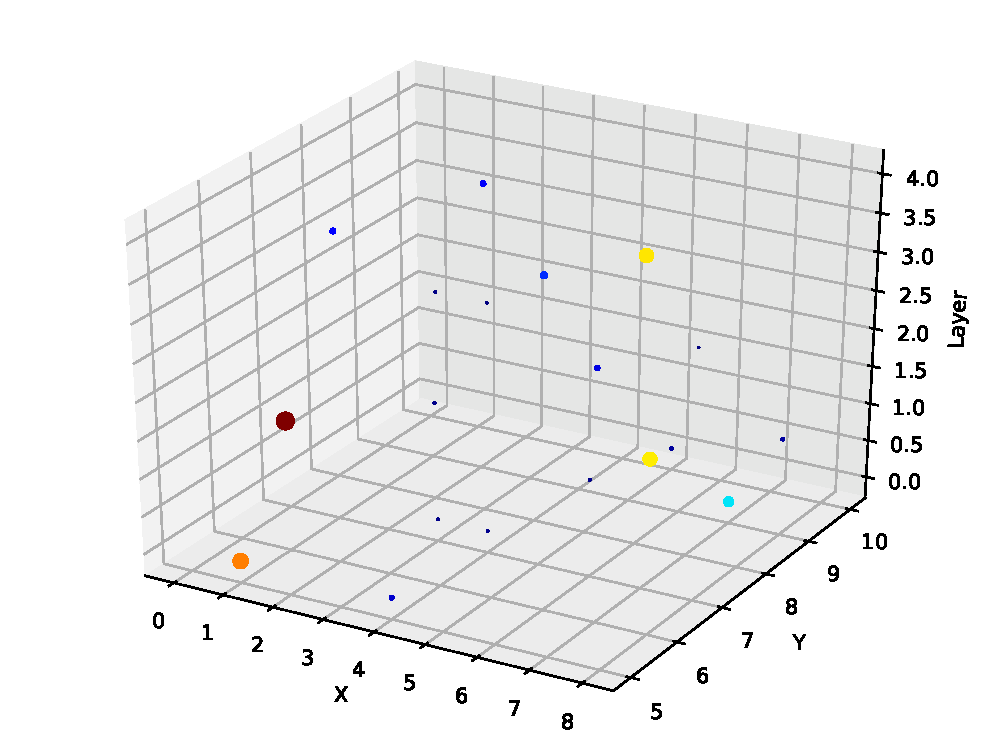
\includegraphics[width=0.45\textwidth]{Images/Calo/Gamma_HCAL.eps}
    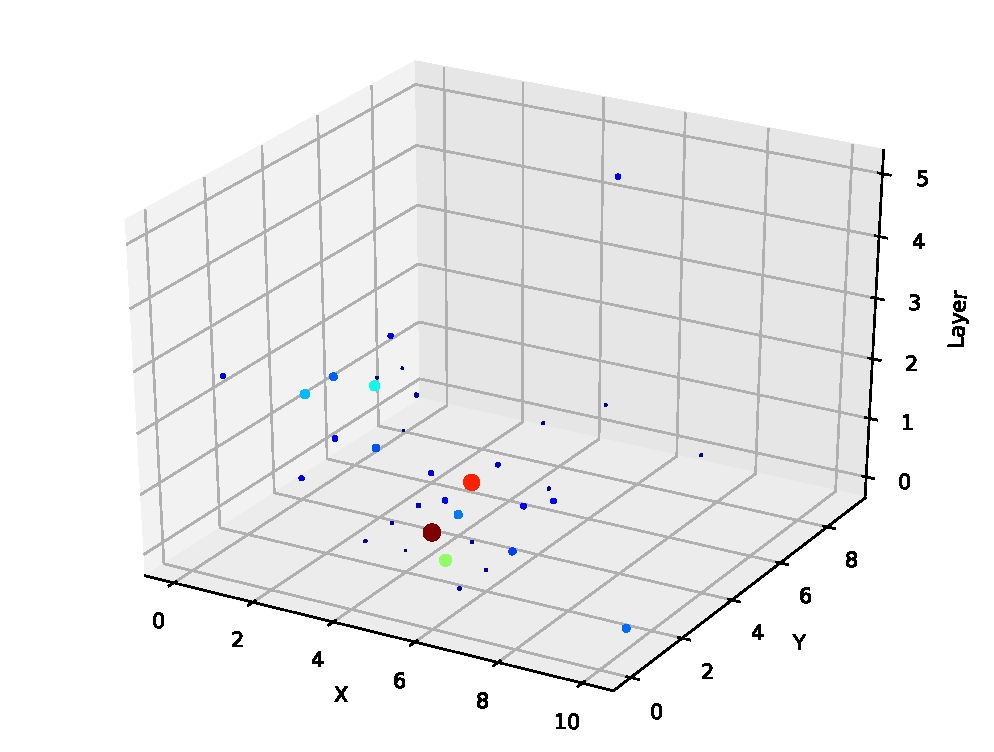
\includegraphics[width=0.45\textwidth]{Images/Calo/Pi0_HCAL.eps} \\
    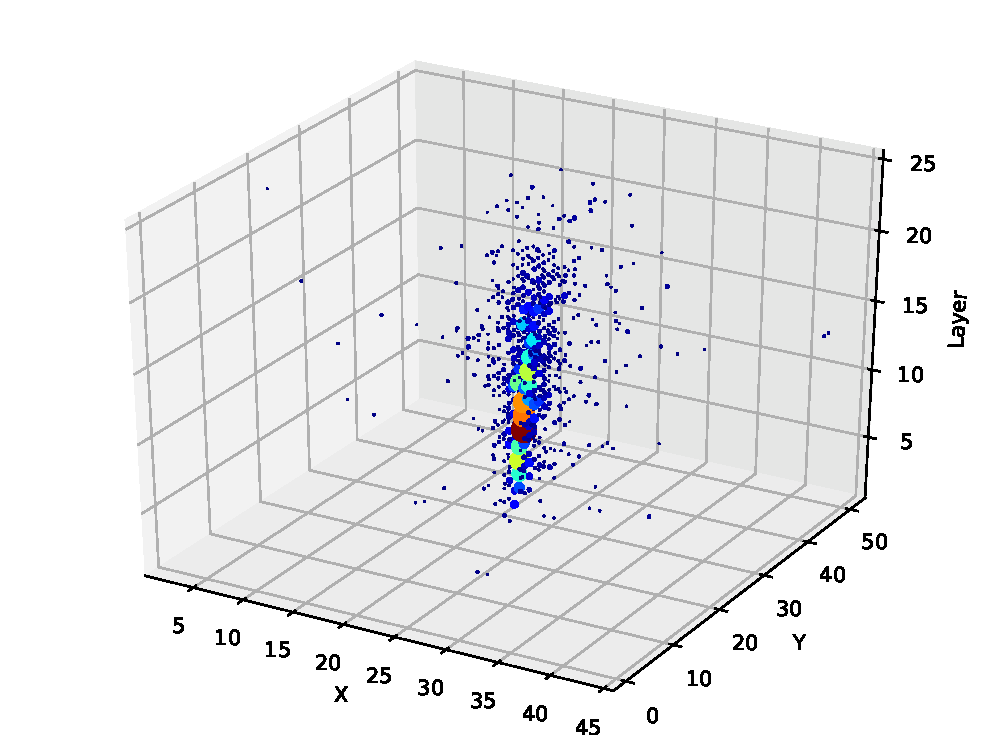
\includegraphics[width=0.45\textwidth]{Images/Calo/Gamma_ECAL.eps}
    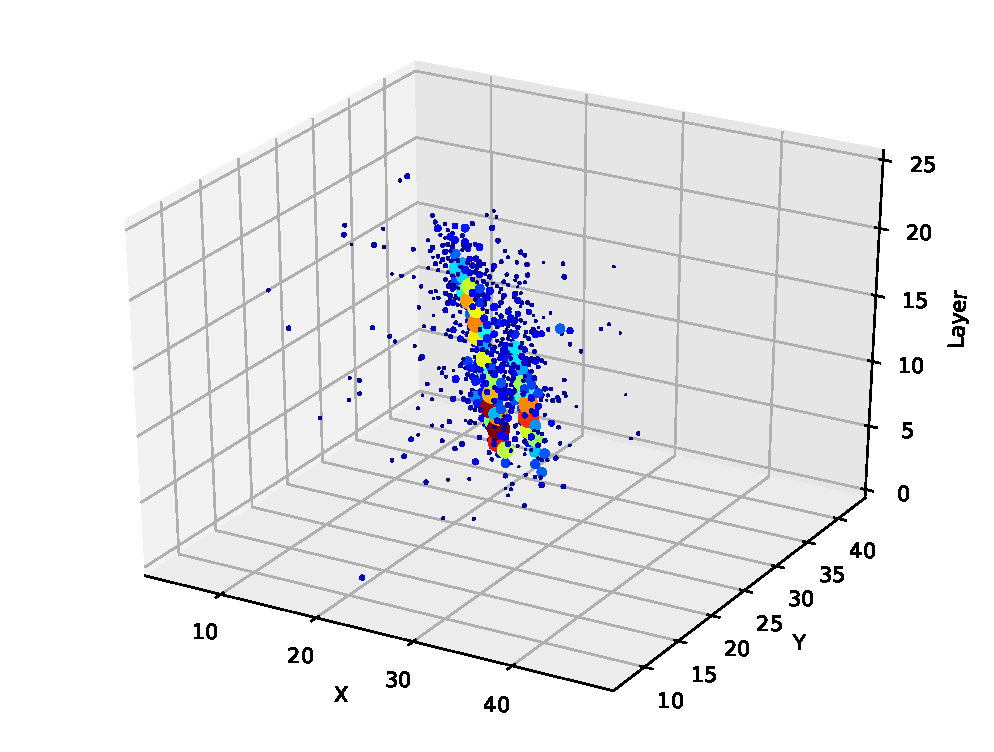
\includegraphics[width=0.45\textwidth]{Images/Calo/Pi0_ECAL.eps}
    \caption{3D image of a photon (left) and neutral pion (right) shower in ECAL (bottom) and HCAL (top).}
    \label{fig:sample}
\end{figure*}

\section{Data Filtering}

We apply a task-dependent filtering of the REC dataset, in order to select the subset of examples for which the task at hand is not trivial. For instance, in general distinguishing a charged pion from an electron is an easy task, and can be accomplished with high accuracy by looking at the HCAL/ECAL energy ratio. On the other hand, a pion with a small HCAL/ECAL ratio leaves most of its energy in the ECAL due to charge conversion processes, and as such would be difficult to distinguish from an electron of equal momentum. Thus, to target the region where a classification algorithm would have most impact, we ignore charged-pion showers with a large HCAL/ECAL energy ratio.

To be more specific, we see in Figure~\ref{fig:HE_ratio} that the ratio of total ECAL energy to total HCAL energy is very different for electrons and charged pions, with the heavier charged pions tending to leave little energy in the ECAL. In order to make the particle-identification task more challenging, we only consider showers with an HCAL/ECAL $< 0.1$ cut. The effects are shown in Figure~\ref{fig:HE_ratio_energy}, where we see the fraction of events from 2-500 GeV that pass this selection. We can see that the selection favors mostly low-energy charged pions, which tend to leave less energy in the HCAL if they manage to make it through the ECAL at all. Discriminating accurately between electrons and charged pions in this range is thus crucial for physics analyses where we are interested in decay products with low energy.

\begin{figure}[htbp]
    \centering
    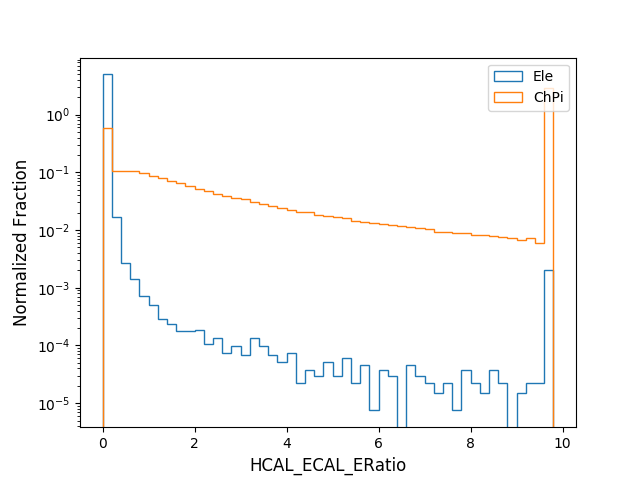
\includegraphics[width=0.7\textwidth]{Images/Calo/ratios.png}
    \caption{HCAL/ECAL energy ratios for electrons and charged pions, plotted on a log scale. The last bin is an overflow bin.}
    \label{fig:HE_ratio}
\end{figure}

\begin{figure}[htbp]
    \centering
    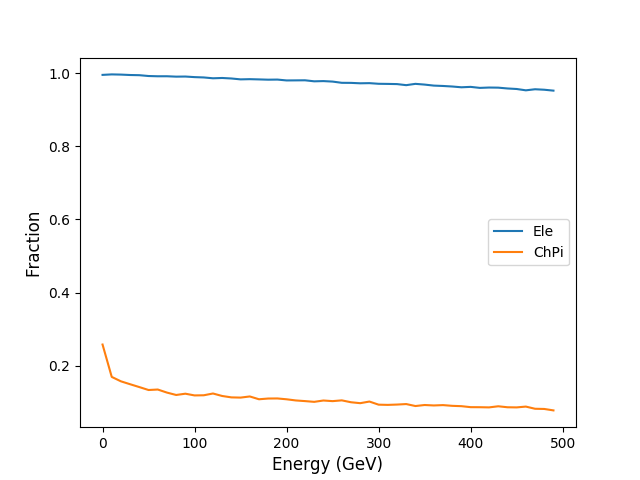
\includegraphics[width=0.45\textwidth]{Images/Calo/ratio_cut_vs_energy.png}
    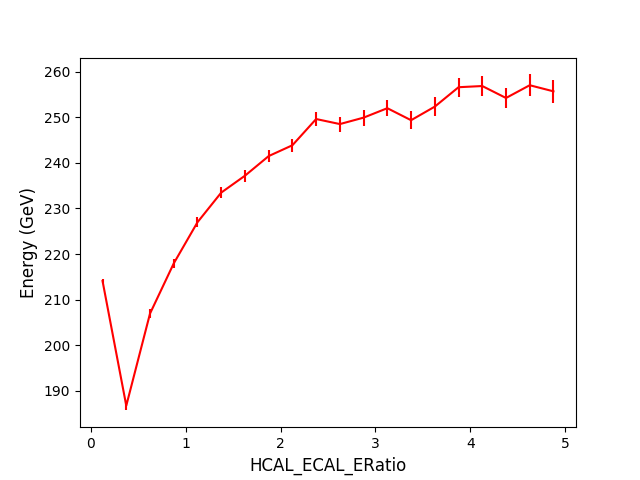
\includegraphics[width=0.45\textwidth]{Images/Calo/mean_energy_vs_ratio.png}
    \caption{Fractions of electrons and charged pions that pass a HCAL/ECAL $< 0.1$ cut at various particle energies (left). Mean charged pion energy as a function of HCAL/ECAL energy ratio (right). We see that if a pion makes it into the HCAL, then we tend to see a positive relation between particle energy and the HCAL/ECAL ratio. About 1 out of 5000 events will leave no hits in the calorimeter window at all, forming the bump in the HCAL/ECAL $= 0$ bin.}
    \label{fig:HE_ratio_energy}
\end{figure}

\begin{figure}[htbp]
    \centering
    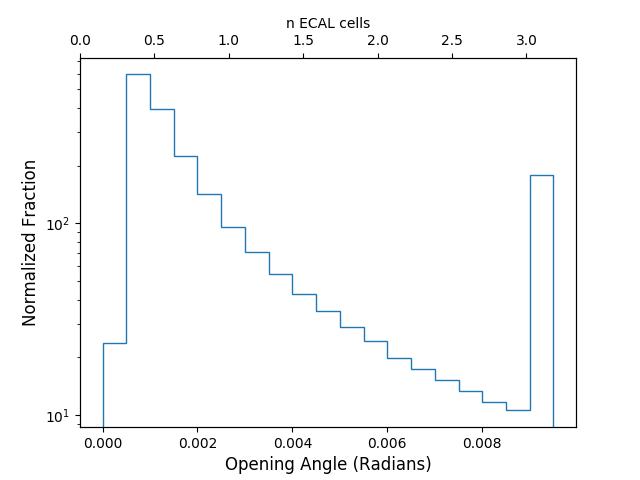
\includegraphics[width=0.7\textwidth]{Images/Calo/zoom_opening_angles.png}
    \caption{Opening angle distribution for neutral pions decaying into two photons, plotted on a log scale with an overflow bin. Plot is zoomed in to show opening angle $< 0.01$. Number of equivalent ECAL cells is shown on the top axis. This plot was generated using pions from the full 2-500 GeV energy range.}
    \label{fig:opening_angle}
\end{figure}

\begin{figure}[htbp]
    \centering
    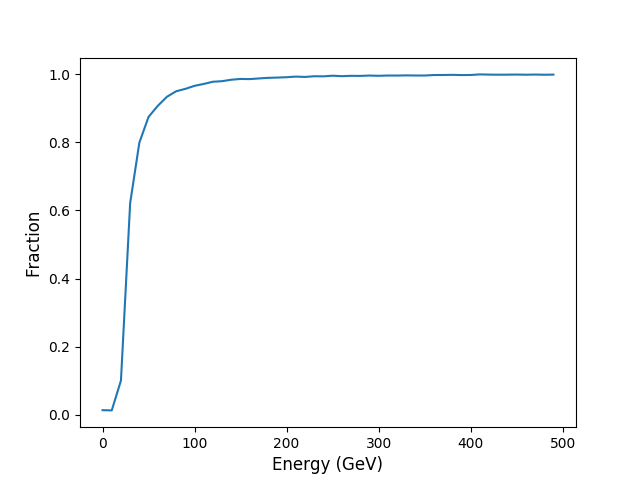
\includegraphics[width=0.45\textwidth]{Images/Calo/opening_angle_cut_vs_energy.png}
    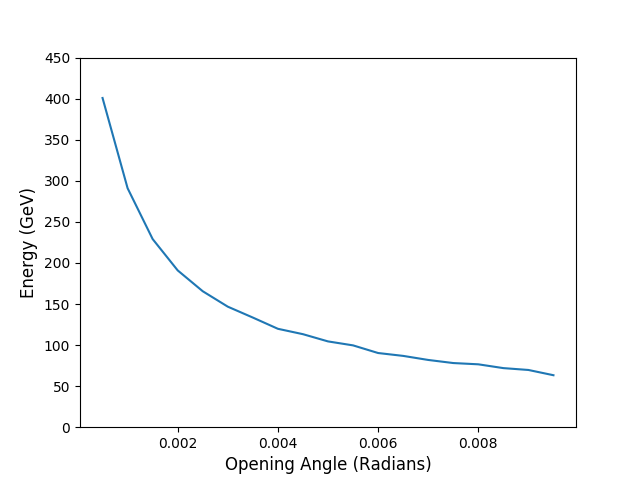
\includegraphics[width=0.45\textwidth]{Images/Calo/mean_energy_vs_opening_angle.png}
    \caption{The fraction of neutral pions passing an opening angle $< 0.01$ radian selection at various particle energies (left). The mean neutral pion energy as a function of opening angle (right).}
    \label{fig:opening_angle_energy}
\end{figure}

Photons and neutral pions are more difficult to distinguish. This is because neutral pions decay preferentially into two photons, with a branching ratio of almost $99\%$. A Lorentz boost due to the momentum of the pion causes the photons to become collimated, to the point where they are only separated by a small angle. If the pion has a low energy, the opening angle between the two photons is larger and the shower is easily identified as originating from a neutral pion. High-energy neutral pions produce more collimated photon pairs, which are more easily mistaken as a single high-energy photon. The opening angle distribution for neutral pions is shown in Figure~\ref{fig:opening_angle}. In order to limit the study to the most challenging case, we filter the neutral-pion dataset by requiring the opening angle between the two photons to be smaller than 0.01 radian.  The effect of  this requirement on the otherwise uniform energy distribution is shown in Figure~\ref{fig:opening_angle_energy}. As expected, the selection mostly removes low-energy neutral pions. 

The ECAL and HCAL 3D arrays are passed directly to our neural networks. We also compute a set of physics-based features, as described in Ref.~\cite{NIPS}. These features are used to train alternative benchmark algorithms representing currently-used ML algorithms in HEP.

\section{Calorimeter Window Size}\label{calo_rec_window_size}

The optimal window size to store for ECAL and HCAL is an important issue, since this impacts not only sample storage size, but also training speed and the maximum batch sizes which we could feed to our GPUs. 

From examinations of our generated samples, we found that an ECAL window of 25x25x25 and an HCAL window of 11x11x60 looked reasonable. To test this hypothesis, we performed training using an unoptimized CNN neural architectures (which will be described later), but with different-sized input samples. The architecture was altered to accommodate larger windows simply by increasing the number of neurons on the input layer. Results trained using an ECAL window of size 25x25x25 and 51x51x25 are shown in Figure~\ref{fig:classification_window}. From the similarity of these curves, we have decided that an expanded ECAL window size does not contain much additional useful information, and is thus not necessary for our problems.

\begin{figure*}[htbp]
    \centering
    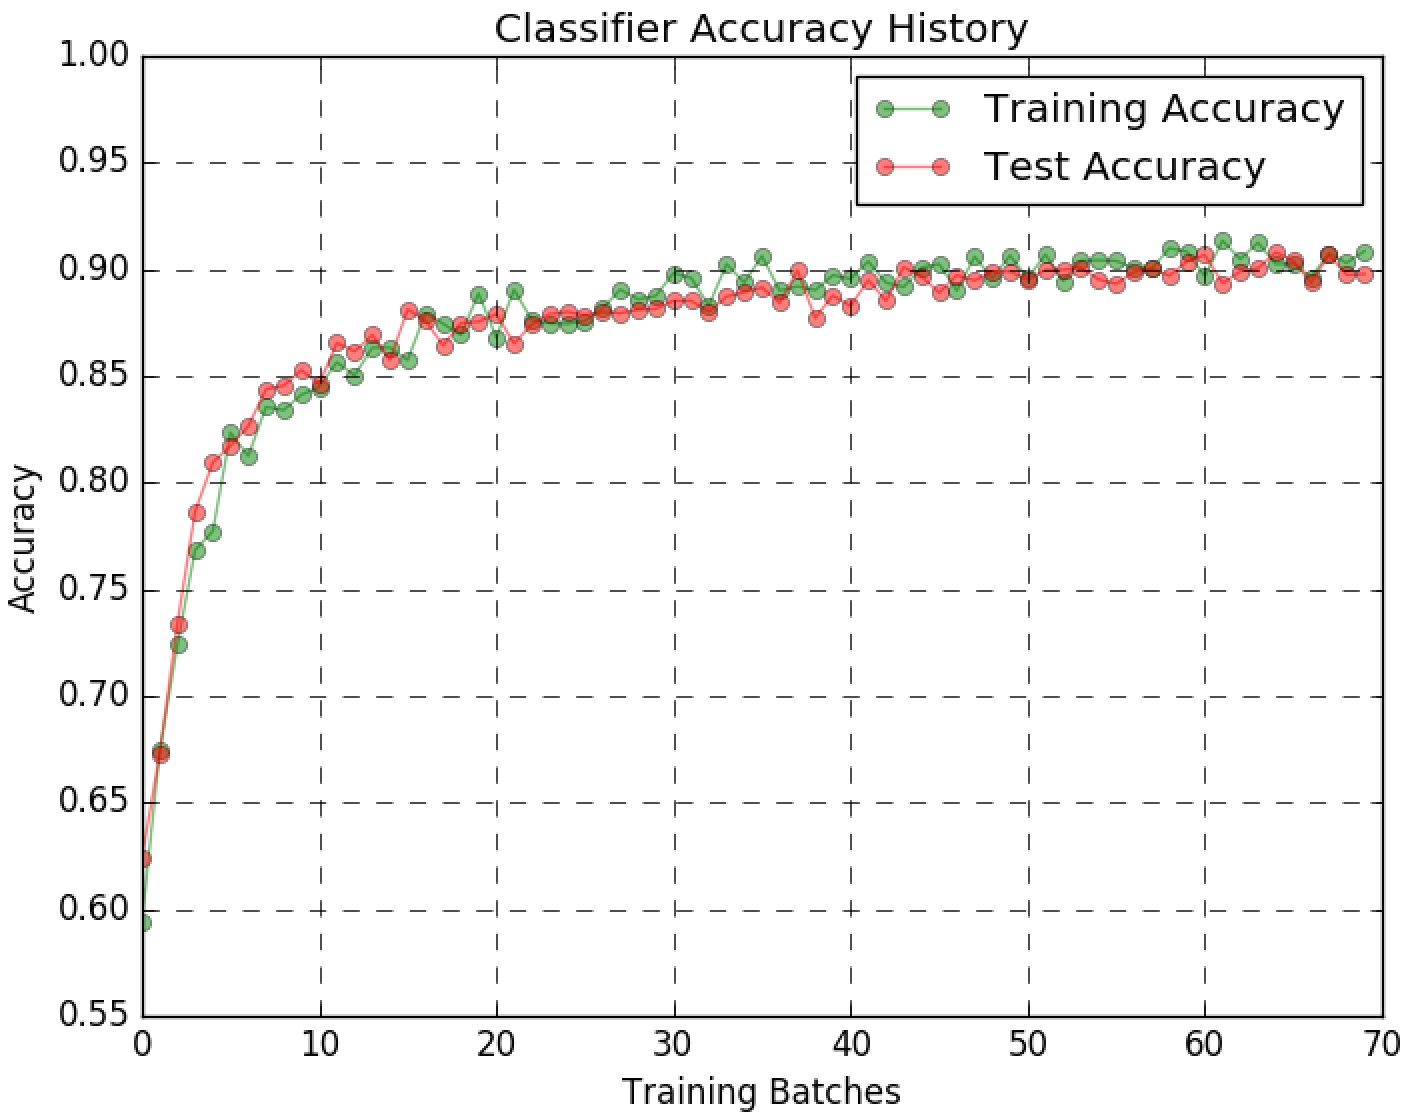
\includegraphics[width=0.45\textwidth]{Images/Calo/accuracy_small_window.png}
    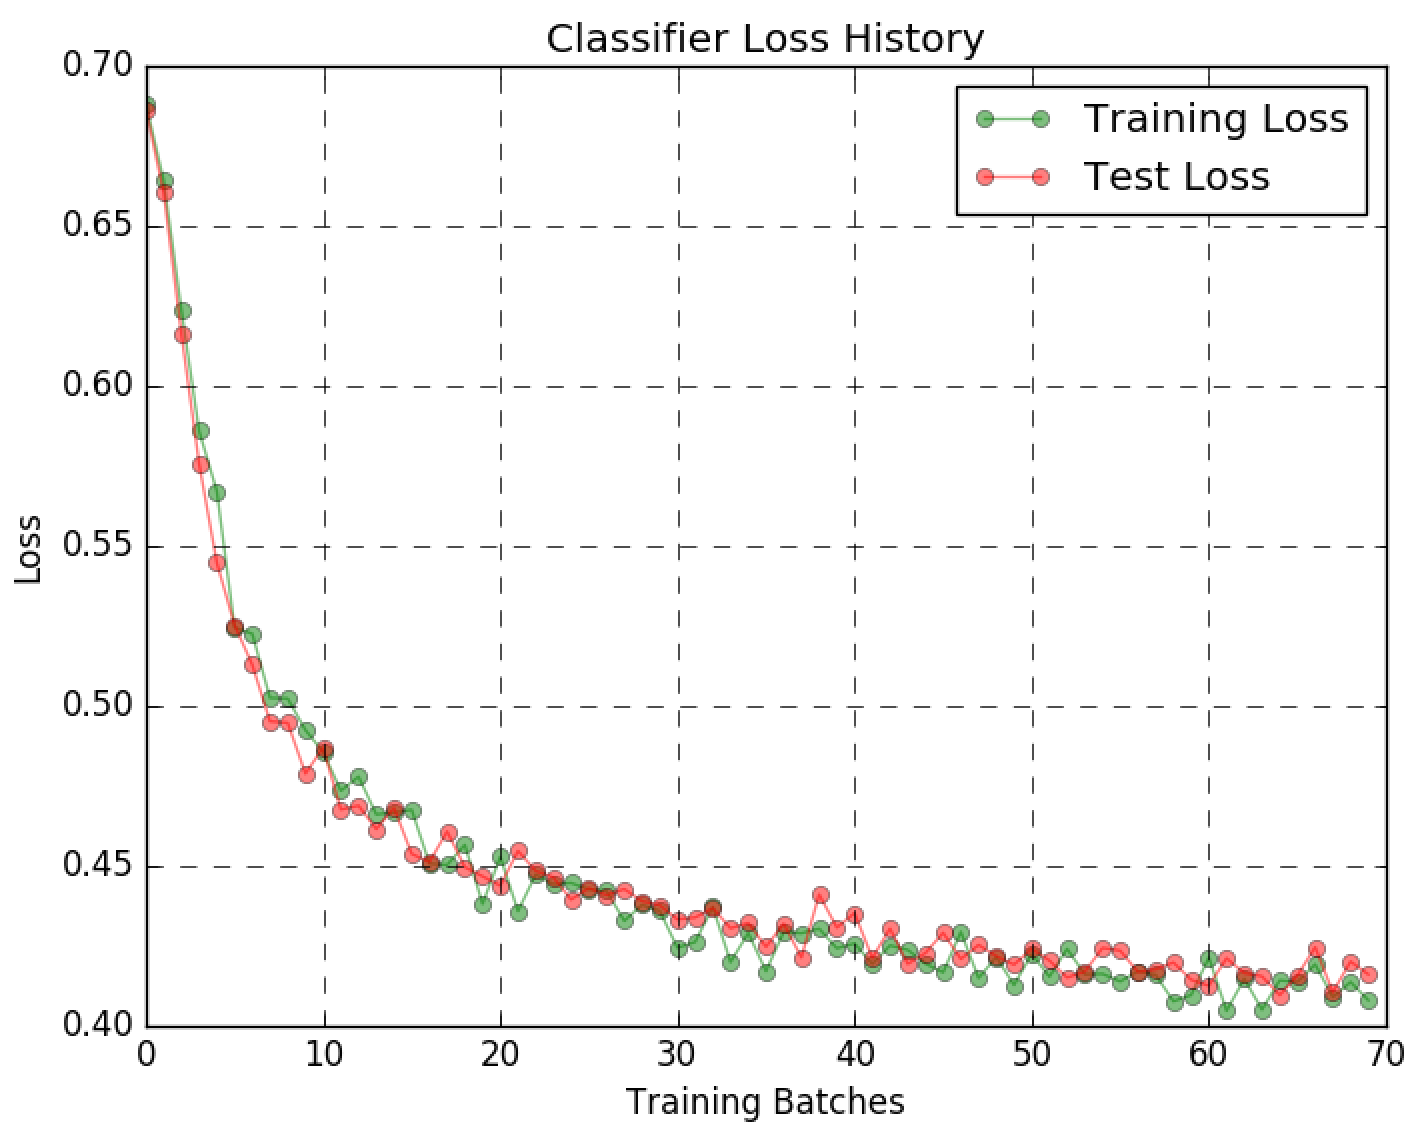
\includegraphics[width=0.45\textwidth]{Images/Calo/loss_small_window.png} \\
    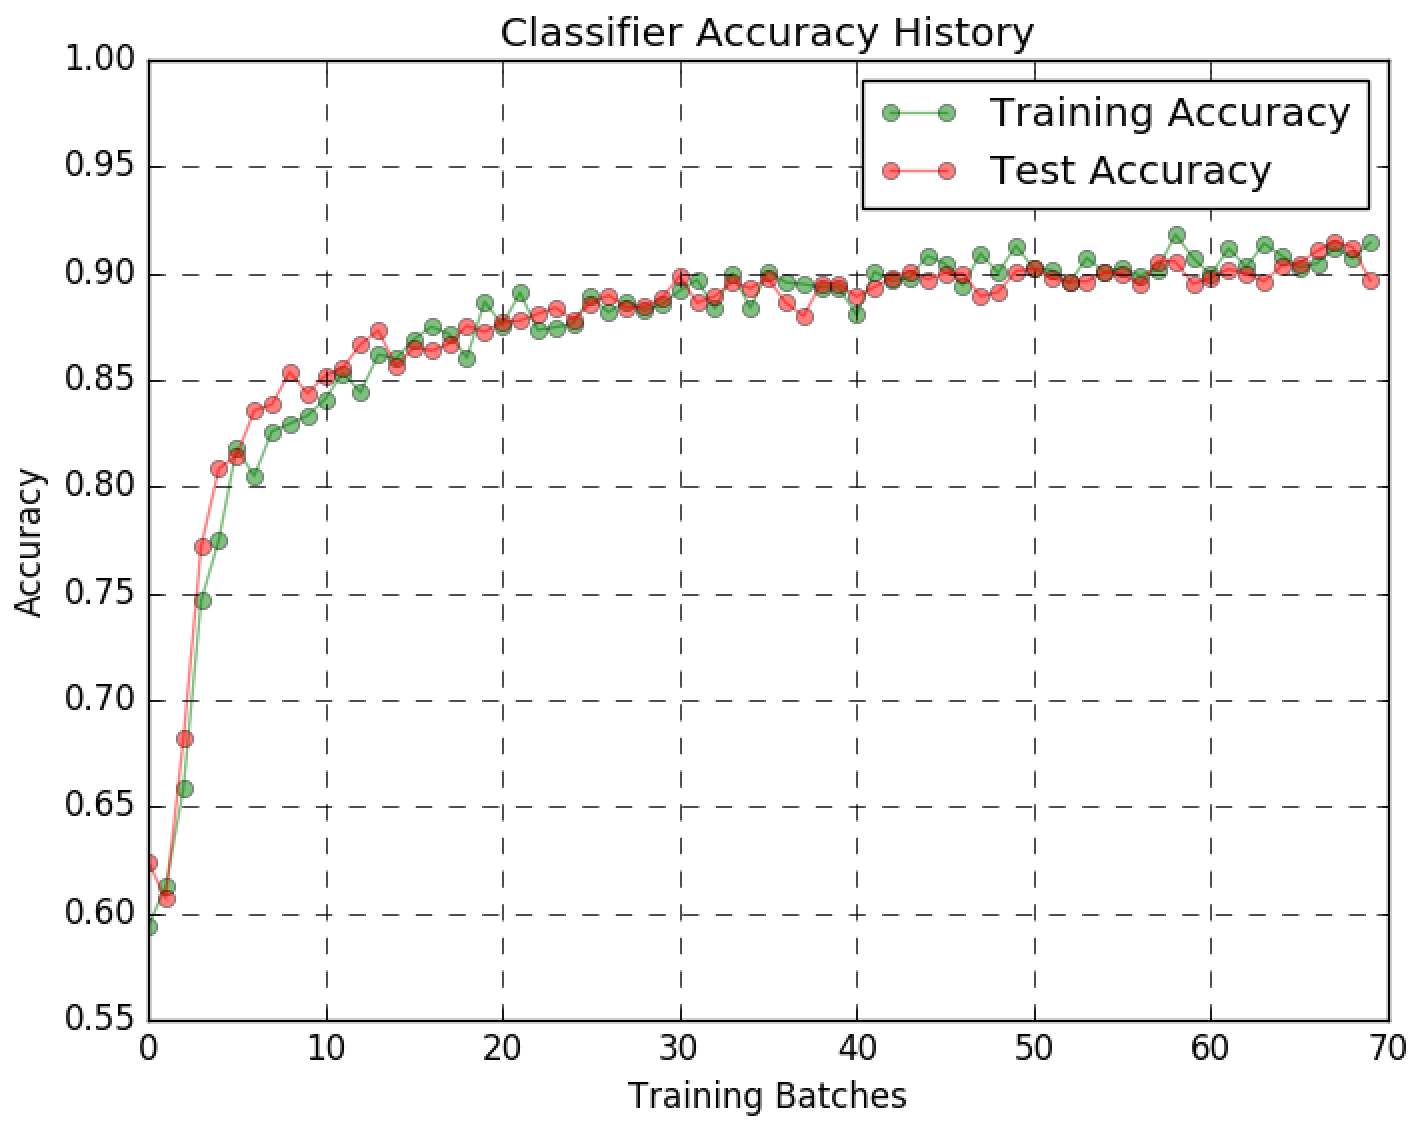
\includegraphics[width=0.45\textwidth]{Images/Calo/accuracy_large_window.png}
    \includegraphics[width=0.45\textwidth]{Images/Calo/loss_large_window.png}
    \caption{Training history for different choices of the input 3D array zise: Accuracy (left) and loss (right) as a function of the training batch for photon/neutral pion classification, using a 25x25x25 (top) and 51x51x25 (bottom) ECAL window size.\label{fig:classification_window}}
\end{figure*}
\chapter{Particle Reconstruction}
\label{sec:reco}

\section{The Tasks}

Our first problem, particle reconstruction, is a crucial part of any high-energy physics analysis. Here, we investigate an end-to-end ML model based on computer vision techniques, where we treat the calorimeter shower as a 3D image. Using a combined architecture, we simultaneously perform particle identification and energy measurement.

When dealing with particle reconstruction, one is interested in identifying a particle's type (electron, photon, etc.) and its momentum. An end-to-end application aiming to provide a full reconstruction of a given particle should thus be able to simultaneously solve a multi-class classification problem and a regression problem. In our study, we filter the REC dataset to make the classification task non-trivial, as described in Section~\ref{sec:data}. Since differentiating charged and uncharged particles is trivial, we judged the classification of our model on its ability to distinguish electrons from charged pions, and photons from neutral pions.

Our reconstruction networks were thus given the following three tasks:
\begin{itemize}
\item {\bf Identify electrons over a background of charged pions}: Charged pions are the most abundant particles produced in LHC collisions. They are typically located in jets, which are collimated sprays resulting from the showering and hadronization processes of quarks and gluons. On the other hand, electrons are rarely produced, and their presence is typically an indication of an interesting event occurring in the collision. A good electron identification algorithm should aim at misidentifying at most 1 in 10,000 pions as an electron. In order to increase the difficulty of our ML problem and to approach the kind of task that one faces at the LHC, we apply the HCAL/ECAL energy ratio cut as described in Section~\ref{sec:data}.
\item {\bf Identify photons over a background of neutral pions}: At particle colliders, the main background to photon identification comes from neutral pions decaying to photon pairs. In general, a generic $\gamma/\pi^0$ classification task is relatively easy, since the presence of two nearby clusters is a clear signature of $\pi^0$. Thus, we focus on events with high $\pi^0$ momentum, using the opening angle selection described in Section~\ref{sec:data}.
\item {\bf Energy measurement}: Once the particle is identified, it is very important to accurately determine its energy (and by extension, its momentum), since this allows physicists to calculate all the relevant high-level features, such as the mass of new particles that generated the detected particles when decaying. In this study, we address this problem on the same dataset used for the classification tasks, restricting the focus to range of energies from 2 to 500 GeV, and at various incident angles ($\eta$). Regression results using various neural network architectures were compared with results from linear regression, comparing both resolution and bias. The models we consider are designed to return the full particle momentum (energy, $\eta$, and $\phi$) of the incoming particle momentum. At this stage, this functionality is not fully exploited and only the energy determination is considered. An extension of our work to include the determination of $\eta$ and $\phi$ could be the matter of future studies.
\end{itemize}

\section{Baselines}

\subsection*{Classification Baseline}\label{app:BDT}

Boosted decision trees were chosen as the baseline of comparison for our classification task, due to their popularity in HEP experiments. Decision trees are effective in producing optimal cut-based decisions based on input features. A BDT is able to increase classification accuracy and stability by aggregating the results from multiple trees. Since a BDT optimizes cut selections, but still depends on the use of traditional pre-calculated features, we are able to use the BDT as a stand-in for standard HEP algorithms using feature-based cuts.

In a previous study~\cite{NIPS}, we compared the performance of a neural model taking energy cell info as input, a feature-based neural model, and a feature-based BDT. In that context, we demonstrated that feature-based BDTs and neural networks performed equally well. Thus, we do not compare feature-based neural networks in this paper, and instead only use feature-based BDTs to represent current state-of-the-art classification algorithms.

The features we use in our baseline BDT classification model~\cite{NIPS} are ones commonly used to characterize particle showers. One additional feature we added is R9, which measures the largest fraction of energy contained within a 3x3 window in a z-axis projection of the shower. This quantity provides a measure of the "concentration" of a shower within a small region. For values near 1, the shower is highly collimated within a single region, as in electromagnetic showers. Smaller values are typical of more spread out showers, as for hadronic and multi-prong showers. A comparison of R9 values between photons and neutral pions can be seen in Figure~\ref{fig:R9}, with examples of events with different R9 values being shown in Figure~\ref{fig:R9_examples}. After training, the discriminating power of various features can be seen in Figure~\ref{fig:BDT_ranking}.

\begin{figure}[htbp]
\centering
\includegraphics[width=0.6\textwidth]{Images/Calo/R9_ratios.png}
\caption{Comparison of R9 distributions between photon and neutral pion events. Photons tend to have more centralized energy depositions.
\label{fig:R9}}
\end{figure}

\begin{figure}[htbp]
\centering
\includegraphics[width=0.4\textwidth]{Images/Calo/R9_0p42.png}
\includegraphics[width=0.4\textwidth]{Images/Calo/R9_0p75.png}
\caption{(Left) (x,y) projection of an event with R9=0.42. (Right) (x,y) projection of an event with R9=0.75.}
\label{fig:R9_examples}
\end{figure}

\begin{figure}[htbp]
\centering
\includegraphics[width=0.7\textwidth]{Images/Calo/BDT_ranking_fixed.png}
\caption{Feature importances for inputs used in BDT training. Values shown are gini importances~\cite{Breiman}.\label{fig:BDT_ranking}}
\end{figure}

\subsection*{Energy Measurement Baseline}\label{app:regression_baseline}

We use linear regression as one of our energy measurement baselines, using ECAL and HCAL total energy as inputs, and where $a$, $b$, and $c$ are trained parameters:

\begin{equation}
E = a \cdot E_{ECAL} + b \cdot E_{HCAL} + c
\label{eq:linreg}
\end{equation}

Linear regression results for each of the particle types are shown in Figure~\ref{fig:reg_linreg}. Each point in the plot represents the mean bias or resolution within an energy bin. In all resolution plots shown in this thesis, the points have been fitted with the following expected resolution function equation:

\begin{equation}
\frac{\sigma(\Delta E)}{E_{\text{true}}} = \frac{a}{\sqrt{E_{\text{true}}}} \oplus b \oplus \frac{c}{E_{\text{true}}}
\label{eq:res}
\end{equation}

\begin{figure}[htbp]
\centering
\includegraphics[width=0.45\textwidth]{Images/Calo/bias_vs_E_allparts_linreg.pdf}
\includegraphics[width=0.45\textwidth]{Images/Calo/res_vs_E_allparts_linreg_fits.pdf}
\caption{Bias (left) and resolution (right) as a function of true energy for linear regression predictions of particle energy for the different particle types, trained on fixed-angle samples. \label{fig:reg_linreg}}
\end{figure}

We also investigated the use of BDTs for energy regression. This application has seen use in some LHC experiments (e.g., to study $H \rightarrow \gamma\gamma$ decays).  We used the XGBoost package in Python, with the following hyperparameters:

\begin{itemize}
\item maximum 1000 iterations, with early stopping if loss doesn't improve on the test set in 10 iterations
\item maximum tree depth of 3
\item minimum child weight of 1 (default)
\item learning rate $\eta = 0.3$ (default)
\end{itemize}

We used the following input features, as we found they gave good performance for electrons, photons, and \pizero. Adding the mean $z$ coordinate to the ECAL and HCAL total energies improved the energy resolution for all energy values, but in particular at high energy, as can be seen in Figure~\ref{fig:reg_xgb_ecalmoms}.

\begin{itemize}
\item total ECAL energy
\item total HCAL energy
\item mean $z$ coordinate of the ECAL shower
\end{itemize}

\begin{figure}[htbp]
\centering
\includegraphics[width=0.45\textwidth]{Images/Calo/bias_vs_E_EleFixed_xgb_ecalmoms_zoom.pdf}
\includegraphics[width=0.45\textwidth]{Images/Calo/res_vs_E_EleFixed_xgb_ecalmoms_fits.pdf}
\caption{Bias (left) and resolution (right) as a function of true energy for the XGBoost regression predictions of particle energy, using different input features for electrons.\label{fig:reg_xgb_ecalmoms}}
\end{figure}

For \chpi, adding the following variables further improved the results:

\begin{itemize}
\item RMS in the $z$ direction of the ECAL shower
\item RMS in the $(x,y)$ plane of the HCAL shower
\item mean $z$ coordinate of the HCAL shower
\end{itemize}

In addition, for \chpi, around 0.5\% of events were found to have almost no reconstructed energy in the selected calorimeter window.  Including these events adversely affected the algorithm training, so they were removed for all the results shown in this and the following sections. Specifically, the raw ECAL+HCAL energy is required to be at least 30\% of the true generated energy.

The results of the XGBoost baseline are compared against linear regression in Figure~\ref{fig:reg_xgb_linreg}. The performance of XGBoost on electrons, photons, and \pizero\ is similar, achieving relative resolutions of about 6--8\% at the lowest energies and 1.0--1.1\% at the highest energies.  Compared to the baseline linear regression, the resolution improves by a factor of about two at low energy and three to four at high energy.  For \chpi, the resolution after XGBoost regression ranges between 20 and 5.4\%, with a relative improvement over linear regression of up to 40\% at high energy.

\begin{figure}[htbp]
\centering
\includegraphics[width=0.45\textwidth]{Images/Calo/bias_vs_E_allparts_linreg_xgb.pdf}
\includegraphics[width=0.45\textwidth]{Images/Calo/res_vs_E_allparts_linreg_xgb_fits.pdf}
\caption{Bias (left) and resolution (right) as a function of true energy for linear regression and XGBoost  predictions of particle energy for the different particle types.\label{fig:reg_xgb_linreg}}
\end{figure}

One drawback of using a BDT algorithm in a real-world setting is that it can not be used for energy values outside the range of the training set. That is, most tree algorithms do not perform extrapolation. This is an inherent disadvantage of the BDT when compared with the neural networks we present in this paper. However, despite this drawback, we use BDT results as a second baseline for comparison in our energy measurement task.

\section{Architecture and Training Details}

As mentioned before, we use a neural architecture which simultaneously performs both particle classification and energy regression. This combined network is trained using the ECAL and HCAL cell arrays as well as the total ECAL energy and total HCAL energy as inputs. The training loss function is written as the sum of a binary cross entropy for particle identification and a mean-square error loss for energy regression. Through experimentation, we found that multiplying the energy component of the loss function by a factor of 200 gave the best results, as it was easier to quickly achieve low loss values for energy regression.

We compare three different architectures for our reconstruction model:

\begin{itemize}
\item A dense (i.e, fully connected) neural network (DNN).
\item A 3D convolutional network (CNN).
\item A network based on GoogLeNet (GN)~\cite{GoogLeNet}, using layers of inception modules.
\end{itemize}

The architecture of each model is defined with a number of floating parameters (e.g. number of hidden layers), which are refined through hyperparameter optimization, as described in Section~\ref{sec:hpscan}. Each model returns three numbers. After applying a softmax activation, two of these elements are interpreted as the classification probabilities of the current two-class problem. The third output is interpreted as the energy of the particle.

Here we describe in detail the three model architectures:

\begin{itemize}
    \item In the DNN model we first flatten our ECAL and HCAL inputs into 1D arrays. We then concatenate these array along with the total ECAL energy, total HCAL energy, estimated $\phi$, and estimated $\eta$, for an array of total size $25 \times 25 \times 25 + 11 \times 11 \times 60 + 4 = 22889$ inputs. This array is fed as input to the first layer of the DNN, followed by a number of hidden layers each followed by a ReLU activation function and a dropout layer. The number of neurons per hidden layer and the dropout probability are identical for each relevant layer. The number of hidden layers, number of hidden neurons per layer, and dropout rate are hyperparameters, tuned as described in the next session.  Finally, we take the output from the last dropout layer, append the total energies and estimated angles again, and feed the concatenated array into a final hidden layer, which results in a three-element output. 
    \item The CNN architecture consists of one 3D convolutional layer for each of the ECAL and HCAL inputs, each followed by a ReLU activation function and a max pooling layer of kernel size $2 \times 2 \times 2$. The number of filters and the kernel size in the ECAL convolutional layer are treated as optimized hyperparameter (see next session). The HCAL layer is fixed at 3 filters with a kernel size of $2 \times 2 \times 6$. The two outputs are then flattened and concatenated along with the total ECAL and HCAL energies, as well as the estimated $\phi$ and $\eta$ coordinates of the incoming particle. The resulting 1D array is passed to a sequence of dense layers each followed by a ReLU activation function and dropout layer, as in the DNN model. The number of hidden layers and the number of neurons on each layer are considered as hyperparameters to be optimized. The output layer consists of three numbers, as for the DNN model. We found that adding additional convolutional layers to this model beyond the first had little impact on performance. This may be because a single layer is already able to capture important information about localized shower structure, and reduces the dimensionality of the event enough where a densely connected net is able to do the rest.
    \item The third model uses elements of the GoogLeNet~\cite{GoogLeNet} architecture. This network processes the ECAL input array with a 3D convolutional layer with 192 filters, a kernel size of 3 in all directions, and a stride size of 1. The result is batch-normalized and sent through a ReLU activation function. This is followed by a series of inception and MaxPool~\cite{conv} layers of various sizes, as will be described in detail below. The output of this sequence is concatenated to the total ECAL energy, the total HCAL energy, the estimated $\phi$ and $\eta$ coordinates, and passed to a series of dense layers like in the DNN architecture, to return the final three outputs. The number of neurons in the final dense hidden layer is the only architecture-related hyperparameter for the GN model. Due to practical limitations imposed by memory constraints, this model does not take the HCAL 3D array as input. This limitation has a small impact on the model performance, since the ECAL array carries the majority of the relevant information for the problems at hand.
\end{itemize}

On all models, the regression task is facilitated by using skip connections to directly append the input total ECAL and HCAL energies to the last layer. The impact of this architecture choice on regression performance is described later in this chapter. In addition to using total energies, we also tested the possibility of using 2D projections of the input energy arrays, summing along the $z$ dimension (detector depth). This choice resulted in worse performance (as described later in this chapter) and was discarded.

\subsection*{GoogLeNet-Based Model Architecture Details}

In our GoogLeNet architecture, we use inception modules. In these modules, inputs go through four separate branches and are then concatenated together. For an inception layer denoted as Inception(A, B, C, D, E, F, G) the branches are defined as follows:

\begin{itemize}
    \item Branch 1: A simple $1 \times 1 \times 1$ convolution, taking A input channels to B output channels. This is followed by a batch normalization and a ReLU activation function.
    \item Branch 2: A $1 \times 1 \times 1$ convolution followed by a $3 \times 3 \times 3$ convolution. The first convolution takes A input channels to C output channels, followed by batch normalization and ReLU. This then goes to the next convolution layer, which outputs D channels using a kernel of size $3 \times 3 \times 3$. This is again followed by batch normalization and ReLU.
    \item Branch 3: A $1 \times 1 \times 1$ convolution followed by a $5 \times 5 \times 5$ convolution. The details are the same as for the other branches, but the first convolution takes A input channels to E output channels, and the next convolution outputs F channels.
    \item Branch 4: A max pool of kernel size $3 \times 3 \times 3$ is followed by a convolution of kernel size $1 \times 1 \times 1$ that takes A input channels to G output channels. This is followed once again by batch normalization and ReLU.
\end{itemize}

Here are full details for each layer of the GoogLeNet-based architecture:

\begin{itemize}
    \item Apply instance normalization to ECAL input.
    \item Convolution with 3D kernel of size 3, going from 1 input channel to 192 channels, with a padding of 1. This is followed by batch normalization and ReLU.
    \item Inception(192,  64,  96, 128, 16, 32, 32)
    \item Inception(256, 128, 128, 192, 32, 96, 64)
    \item Max pooling with a 3D kernel of size 3, a stride of 2, and padding of 1.
    \item Inception(480, 192,  96, 208, 16,  48,  64)
    \item Inception(512, 160, 112, 224, 24,  64,  64)
    \item Inception(512, 128, 128, 256, 24,  64,  64)
    \item Inception(512, 112, 144, 288, 32,  64,  64)
    \item Inception(528, 256, 160, 320, 32, 128, 128)
    \item Max pooling with a 3D kernel of size 3, a stride of 2, and padding of 1.
    \item Inception(832, 256, 160, 320, 32, 128, 128)
    \item Inception(832, 384, 192, 384, 48, 128, 128)
    \item Average pooling with a 3D kernel of size 7 and a stride of 1.
    \item The output array is flattened and concatenated with input $\phi$, $\eta$, total ECAL energy, and total HCAL energy.
    \item A densely connected layer with 1024 outputs, followed by ReLU.
    \item The output array is once again concatenated with the same input values.
    \item A final densely connected layer outputs 5 values, as in the architectures of the other two models.
\end{itemize}

The full architecture is shown in Figure~\ref{fig:gn_with_inceptin}.

\begin{figure}[htbp]
\centering
\includegraphics[width=0.45\textwidth]{Images/Calo/GN_architecture.png}
\includegraphics[width=0.45\textwidth]{Images/Calo/inception_architecture.png}
\caption{GoogLeNet-based architecture (top) and component inception architecture (bottom).
}
\label{fig:gn_with_inceptin}
\end{figure}

\subsection*{Use of HCAL in Reconstruction}

Since the GoogLeNet architecture was quite large and required significant memory usage and computational power, we decided to investigate the possibility of leaving out HCAL cell-level information, since most of the particle shower occurs in the ECAL. After optimizing our DNN, we took our best-performing DNN architecture and ran ten training sessions with HCAL information, and ten training sessions without HCAL. Averaged training curves from these runs are shown in Figures~\ref{fig:HCAL_study_elechpi} and~\ref{fig:HCAL_study_gammapi0}. These studies demonstrated that including the HCAL caused little to no improvement in classification accuracy. For memory purposes, we thus kept HCAL cell-level information out of our GN architecture. Summed HCAL energy was still fed as an input to the combined classification-regression net, for use in energy regression.

We must note here that though HCAL information is useful for particle reconstruction in general, the reason we do not see much use for it here is because we are mostly looking at events where the majority of energy is deposited in the ECAL. This is particularly true due to the HCAL/ECAL ratio we have applied to electron/charged pion events.

\begin{figure}[htbp]
\centering
\includegraphics[width=0.45\textwidth]{Images/Calo/HCAL_study_elechpi_accuracy.png}
\includegraphics[width=0.45\textwidth]{Images/Calo/HCAL_study_elechpi_loss.png}
\caption{Accuracy and loss curves for electron/charged pion classification, with and without HCAL cells, using best DNN architecture.}
\label{fig:HCAL_study_elechpi}
\end{figure}

\begin{figure}[htbp]
\centering
\includegraphics[width=0.45\textwidth]{Images/Calo/HCAL_study_gammapi0_accuracy.png}
\includegraphics[width=0.45\textwidth]{Images/Calo/HCAL_study_gammapi0_loss.png}
\caption{Accuracy and loss curves for photon/neutral pion classification, with and without HCAL cells, using best DNN architecture.}
\label{fig:HCAL_study_gammapi0}
\end{figure}

\subsection*{Regression with Large Sample Windows}

We saw earlier that classification was not affected by a larger calorimeter window. We wanted to see the effects of using a smaller window on reconstruction as well. We found that for both DNN and CNN, to achieve the best performance for energies above 150~GeV, a minimum $(x,y)$ size of 25x25 in the ECAL and 5x5 in the HCAL is needed. For energies below 150~GeV, the optimal performance is observed for a window size of 51x51 in the ECAL and 11x11 in the HCAL. This is presumably due to wider showers at low energy.  The impact of the choice of window size is shown for DNN in Figure~\ref{fig:reg_dnn_numcells}, with the results for CNN being similar.  Drawbacks to the larger window size, however, include larger files, more memory usage, and that training takes about 5 times longer per epoch.

\begin{figure}[htbp]
\centering
\includegraphics[width=0.45\textwidth]{Images/Calo/bias_vs_E_EleFixed_nn_numcells_zoom.pdf}
\includegraphics[width=0.45\textwidth]{Images/Calo/res_vs_E_EleFixed_nn_numcells_fits.pdf}
\caption{Bias (left) and resolution (right) as a function of true energy for DNN energy predictions for electrons, with varying input window sizes.
}
\label{fig:reg_dnn_numcells}
\end{figure}

Showers for \chpi\ were observed to be wider than the other particle types, especially at low energies, and so we compare the effect of the calorimeter window size choice for \chpi\ in Figure~\ref{fig:reg_nn_numcells_chpi_large_window}. The wider window of 51x51 in $(x,y)$ in the ECAL and 11x11 in the HCAL gives better performance, especially at the lowest energies where the resolution is improved by a factor of about 2 over the smaller window size (25x25 ECAL, 5x5 HCAL).

\begin{figure}[htbp]
\centering
\includegraphics[width=0.45\textwidth]{Images/Calo/bias_vs_E_ChPiFixed_Cut30_nn_numcells.pdf}
\includegraphics[width=0.45\textwidth]{Images/Calo/res_vs_E_ChPiFixed_Cut30_nn_numcells_fits.pdf}
\caption{Bias (left) and resolution (right) as a function of true energy for energy predictions for \chpi, comparing calorimeter window sizes for the CNN and DNN models.
}
\label{fig:reg_nn_numcells_chpi_large_window}
\end{figure}

Overall, though the larger window did make a bit of difference, the improvement was not large enough to overcome the downsides, and we decided to stick with smaller windows for training.

\subsection*{Skip Connections}

A design choice that improved convergence time, and improved performance for the CNN, was including ``skip connections'' for the total ECAL and HCAL energies in the network.  In addition to the individual cell energy values, the total ECAL and HCAL energy values are given as inputs to both the first dense layer and to the last output layer.  The weights for these energy values are initialized to 1, as linear regression with coefficients near 1 is observed to reasonably reproduce the true energy values.  The impact of adding skip connections on performance using a CNN architecture for a fixed number of 5 training epochs is shown in Figure~\ref{fig:reg_cnn_skip}.

\begin{figure}[htbp]
\centering
\includegraphics[width=0.45\textwidth]{Images/Calo/bias_vs_E_EleFixed_cnn_skip_zoom.pdf}
\includegraphics[width=0.45\textwidth]{Images/Calo/res_vs_E_EleFixed_cnn_skip_fits.pdf}
\caption{Bias (left) and resolution (right) as a function of true energy for CNN energy predictions for electrons, with or without skip connections in the architecture.
}
\label{fig:reg_cnn_skip}
\end{figure}

\subsection*{Training Using Energy Summed in z}

For regression, we tried using only the energy summed in layers in the $z$ direction, instead of the full array of cell energies, as the mean $z$ coordinate was seen to be the most important additional feature in the XGBoost baseline.  The performance is better than the XGBoost baseline at high energies but worse than using the full cell-level information, as shown in Figure~\ref{fig:reg_dnn_inputs}.

\begin{figure}[htbp]
\centering
\includegraphics[width=0.45\textwidth]{Images/Calo/bias_vs_E_EleFixed_nn_inputs_zoom.pdf}
\includegraphics[width=0.45\textwidth]{Images/Calo/res_vs_E_EleFixed_nn_inputs_fits.pdf}
\caption{Bias (left) and resolution (right) as a function of true energy for DNN energy predictions for electrons, using as input either the energy summed in layers of $z$, or the full cell information.\label{fig:reg_dnn_inputs}}
\end{figure}

\section{Hyperparameter Scans}\label{sec:hpscan}

In order to fine-tune our models, we scanned over a hyperparameter space for each architecture. In addition to architecture parameters, learning rate and decay rate were additional hyperparameters for each architecture. For simplicity, we used classification accuracy for the $\gamma$ vs. $\pi^0$ problem as a metric to determine the overall best hyperparameter set for each architecture. This is because a model optimized for this task was found to generate good results for the other tasks as well, since $\gamma$ vs. $\pi^0$ classification was found to be the most difficult problem.

Training was performed at each hyperparameter point ten times, in order to obtain an estimate of the uncertainty associated with each quoted performance value. For each scan point, the DNN and CNN architectures trained on 400,000 events, using another sample of 400,000 events for testing. DNN and CNN scan points trained for three epochs each, taking about seven hours each. GN trained on 100,000 events and tested on another 100,000. Due to a higher training time, each GN scan point only trained for a single epoch, taking about twenty hours.

For CNN and DNN training, we used batches of 1,000 events when training. However, due to GPU memory limitations, we could not do the same with GN. Instead, we split each batch into 100 minibatches of ten events each. A single minibatch was loaded on the GPU at a time, and gradients were added up after back-propagation. We waited until after each batch was fully calculated to update network weights using the combined gradients. The best settings were found to be as follows:

\begin{itemize}
    \item For DNN, 4 hidden layers, 512 neurons per hidden layer, a learning rate of 0.0002, decay rate of 0, and a dropout probability of 0.04.
    \item For CNN, 4 hidden layers and 512 neurons per hidden layer, a learning rate of 0.0004, decay rate of 0, a dropout probability of 0.12, 6 ECAL filters with a kernel size of $6 \times 6 \times 6$.
    \item For GN, 1024 neurons in the hidden layer, 0.0001 learning rate, and 0.01 decay rate. 
\end{itemize}
%For CNN and GN, a very mild dependence on the number of neurons per hidden layer is observed. 

\begin{figure*}[htbp]
\centering
\includegraphics[width=0.45\textwidth]{Images/Calo/DNN_hl_nhl.pdf}
\includegraphics[width=0.45\textwidth]{Images/Calo/DNN_lr_dp.pdf} \\
\includegraphics[width=0.45\textwidth]{Images/Calo/CNN_lr_dp.pdf}
\includegraphics[width=0.45\textwidth]{Images/Calo/CNN_nECALfilt_nECALkern.pdf} \\
\includegraphics[width=0.45\textwidth]{Images/Calo/GN_nhl_lr.pdf}
\includegraphics[width=0.45\textwidth]{Images/Calo/GN_lr_dr.pdf}
\caption{Selected hyperparameter scan results for DNN (top), CNN (center), and the GoogLeNet-based architecture (bottom). In each figure, the classification accuracy is displayed as a function of the hyperparameters reported on the two axes.}
\label{fig:scan_hyperparameter}
\end{figure*}

The DNN, CNN, and GN-based models had 9823774 ($\sim$10M), 3003692 ($\sim$3M), and 14956286 ($\sim$15M) trainable parameters respectively after the hyperparameter scans.

Selected hyperparameter scan slices are shown in Figure~\ref{fig:scan_hyperparameter}. 
These 2D scans were obtained setting all values besides the two under consideration (i.e., those on the axes) to be fixed at default values: a dropout rate of 0.08, a learning rate of 0.0004, a decay rate of 0.04, three dense layers for CNN and DNN, and 512 neurons per hidden layer. For GN, the default number of ECAL filters was 3, with a kernel size of 4.
%An ECAL window size of 25 was used in all instances, to allow fair comparison between DNN, CNN, and GN, as larger ECAL sizes posed a memory problem when training GN.

After performing the hyperparameter scan, we trained each architecture using its optimal hyperparameters for a greater number of epochs. The evolution of the training and validation accuracy as a function of the batch number for these extended trainings is shown in Figure~\ref{fig:training_curves_comparison_gamma_pi0}.

\begin{figure}[htbp]
\centering
\includegraphics[width=0.45\textwidth]{Images/Calo/DNN_accuracy_batches_long.png}
\includegraphics[width=0.45\textwidth]{Images/Calo/CNN_accuracy_batches_long.png}
\includegraphics[width=0.45\textwidth]{Images/Calo/GN_accuracy_batches_long.png}
\caption{Training curves for best DNN (top), CNN (middle), and GoogLeNet (bottom) hyperparameters, trained on variable-angle $\gamma$/$\pi^0$ samples. We see that the DNN over-trains quickly and saturates at a relatively low accuracy, while the CNN takes longer to over-train and reaches a higher accuracy, and GoogLeNet performs best of all. Each 400 batches corresponds to a single epoch.}
\label{fig:training_curves_comparison_gamma_pi0}
\end{figure}
\chapter{Reconstruction Results}

\section{Classification}

We apply the best architectures (as found via the hyperparameter scans in the previous section) separately to our electron vs. charged pion and photon vs. neutral pion reconstruction problems.

Figure~\ref{fig:architectures_ROC_comparisons} shows ROC curve comparisons for the two classification tasks. As expected, the electron vs. charged pion classification problem was found to be a simple task, resulting in an area under the curve (AUC) close to $100\%$. For a baseline comparison, the curve obtained for a BDT is also shown. This BDT was optimized using the {\it scikit-optimize} package~\cite{skopt}, and was trained using high-level features computed from the raw 3D arrays. It represents the performance of current (non-deep-learning) ML approaches on these problems.

\begin{figure}[htbp]
\centering
\includegraphics[width=0.45\textwidth]{Images/Calo/architectures_ROC_comparison_gamma_pi0_long.pdf}
\includegraphics[width=0.45\textwidth]{Images/Calo/architectures_ROC_comparison_ele_chpi_xlog.pdf}
\caption{ROC curve comparisons for $\gamma$ vs. $\pi^0$ (left) and $e$ vs. $\pi^\pm$ (right) classification using DNN, CNN, BDT, and GoogLeNet (GN). Samples include particle energies from 2 to 500 GeV, and an inclusive $\eta$ range.}
\label{fig:architectures_ROC_comparisons}
\end{figure}

Our deep learning models outperform the BDT, with the GN architecture performing best on both problems. Figure~\ref{fig:accuracy_bins} shows the best-model performance as a function of the energy and $\eta$ of the incoming particle, for both classification problems. These figures show that classification accuracy is maintained over a wide range of particle energies and angles. The models appear to perform a bit worse at higher energies for the photon vs. neutral pion case, due to the fact that the pion to two photon decay becomes increasingly collimated at higher energies. Similarly, the performance is slightly worse when particles impact the detector perpendicularly than when they enter at a wide angle, because the shower cross section on the calorimeter inner surface is reduced at $90^{\mathrm o}$, making it harder to distinguish shower features.

\begin{figure*}[htbp]
\centering
\includegraphics[width=0.45\textwidth]{Images/Calo/gamma_pi0_accuracy_energy_bins.pdf}
\includegraphics[width=0.45\textwidth]{Images/Calo/gamma_pi0_accuracy_eta_bins.pdf} \\
\includegraphics[width=0.45\textwidth]{Images/Calo/ele_chpi_accuracy_energy_bins.pdf}
\includegraphics[width=0.45\textwidth]{Images/Calo/ele_chpi_accuracy_eta_bins.pdf}
\caption{Classification accuracy of best performing network for $\gamma$ vs. $\pi^0$ (top) and $e$ vs. $\pi^\pm$ (bottom), in bins of energy (left) and $\eta$ (right).}
\label{fig:accuracy_bins}
\end{figure*}

\section{Regression}

Figure~\ref{fig:reg_dnn_vs_cnn_variable} shows the energy regression performance for each particle type, using each hyperparameter-optimized architecture. We compare against a linear regression and a BDT (labelled as "XGBoost") baseline, as described previously.

\begin{figure*}[htbp]
\centering
\includegraphics[width=0.45\textwidth]{Images/Calo/bias_vs_E_Ele_variable.pdf}
\includegraphics[width=0.45\textwidth]{Images/Calo/res_vs_E_Ele_variable.pdf} \\
\includegraphics[width=0.45\textwidth]{Images/Calo/bias_vs_E_ChPi_variable.pdf}
\includegraphics[width=0.45\textwidth]{Images/Calo/res_vs_E_ChPi_variable.pdf} \\
\includegraphics[width=0.45\textwidth]{Images/Calo/bias_vs_E_Gamma_variable.pdf}
\includegraphics[width=0.45\textwidth]{Images/Calo/res_vs_E_Gamma_variable.pdf}\\
\includegraphics[width=0.45\textwidth]{Images/Calo/bias_vs_E_Pi0_variable.pdf}
\includegraphics[width=0.45\textwidth]{Images/Calo/res_vs_E_Pi0_variable.pdf}
\caption{Regression bias (left) and resolution (right) as a function of true energy for energy predictions on the REC dataset with variable-angle incident angle. From top to bottom: electrons, charged pions, photons, and neutral pions. Algorithms compared are linear regression, XGBoost (BDT), DNN, CNN, and GoogLeNet (GN).\label{fig:reg_dnn_vs_cnn_variable}}
\end{figure*}

Since the energy regression problem is not as complex as the classification problem, the three architectures (DNN, CNN, GN) perform fairly similarly, with the exception of the GN performance on \chpi, which is a bit worse. The performance is overall worse for \chpi, both with the networks and with the benchmark baselines (linear regression and XGBoost).

A closer look at the performance boost given by each network can be obtained examining the case of particles entering the calorimeter inner surface at $90^{\mathrm o}$, i.e. with $\eta=0$~\footnote{For these additional fixed-angle regression plots, we did not train GoogLeNet architectures.}. In this case, the problem is more constrained and both the networks and the baseline algorithms are able to perform accurately. The results for fixed angle samples are shown in Figure~\ref{fig:reg_dnn_vs_cnn_fixed}.

\begin{figure*}[htbp]
\centering
\includegraphics[width=0.45\textwidth]{Images/Calo/bias_vs_E_EleFixed_nn_vs_cnn_zoom.pdf}
\includegraphics[width=0.45\textwidth]{Images/Calo/res_vs_E_EleFixed_nn_vs_cnn_fits.pdf} \\
\includegraphics[width=0.45\textwidth]{Images/Calo/bias_vs_E_ChPiFixed_Cut30_nn_vs_cnn.pdf}
\includegraphics[width=0.45\textwidth]{Images/Calo/res_vs_E_ChPiFixed_Cut30_nn_vs_cnn_fits.pdf} \\
\includegraphics[width=0.45\textwidth]{Images/Calo/bias_vs_E_GammaFixed_nn_vs_cnn_zoom.pdf}
\includegraphics[width=0.45\textwidth]{Images/Calo/res_vs_E_GammaFixed_nn_vs_cnn_fits.pdf} \\
\includegraphics[width=0.45\textwidth]{Images/Calo/bias_vs_E_Pi0Fixed_nn_vs_cnn_zoom.pdf}
\includegraphics[width=0.45\textwidth]{Images/Calo/res_vs_E_Pi0Fixed_nn_vs_cnn_fits.pdf}
\caption{Regression bias (left) and resolution (right) as a function of true energy for energy predictions on the REC dataset with fixed incident angle ($90^\mathrm{o}$). From top to bottom: electrons, charged pions, photons, and neutral pions.\label{fig:reg_dnn_vs_cnn_fixed}}
\end{figure*}

\subsection*{Cross Training on Different Particle Types}

All the tests so far have assumed that we know exactly what type of particle led to the reconstructed energy deposits.  In a real world situation, the particle identities are not known with complete confidence.  To see how the algorithms above would cope with that situation, we tried training each algorithm on an input sample of electron events, and then we used the trained algorithm to predict the energies for other particle types.

The results are shown in Figure~\ref{fig:reg_nn_cross_gamma} for predicting photon energies and Figure~\ref{fig:reg_nn_cross_pi0} for predicting \pizero\ energies, and are compared to algorithms that are both trained and tested on the same particle type.  In each case, a DNN or CNN trained on electrons is able to achieve the same resolution as a CNN trained on photons or \pizero.  The bias is slightly larger in some cases.

\begin{figure}[hbp]
\centering
\includegraphics[width=0.45\textwidth]{Images/Calo/bias_vs_E_EleGammaFixed_nn_cross_zoom.pdf}
\includegraphics[width=0.45\textwidth]{Images/Calo/res_vs_E_EleGammaFixed_nn_cross_fits.pdf}
\caption{Bias (left) and resolution (right) as a function of true energy, for electrons and photons.  The particles used to train and test each algorithm are given in the legend.
}
\label{fig:reg_nn_cross_gamma}
\end{figure}

\begin{figure}[htbp]
\centering
\includegraphics[width=0.45\textwidth]{Images/Calo/bias_vs_E_ElePi0Fixed_nn_cross_zoom.pdf}
\includegraphics[width=0.45\textwidth]{Images/Calo/res_vs_E_ElePi0Fixed_nn_cross_fits.pdf}
\caption{Bias (left) and resolution (right) as a function of true energy, for electrons and \pizero.  The particles used to train and test each algorithm are given in the legend.
}
\label{fig:reg_nn_cross_pi0}
\end{figure}

Models trained on electrons, photons, or \pizero\ were found to not describe \chpi\ well at all.  This is not surprising given that \chpi\ has a hadronic shower, with a large fraction of energy deposited in the HCAL, compared to the other particles depositing almost all of their energy in the ECAL.

We also checked whether the energy regression was different for photons that have converted into an $e^{+}e^{-}$ pair through interaction with the detector material.  These conversion photons comprise about 9\% of the photon sample.  We tried training and/or evaluating regression models separately on converted photons compared to all photons (which are dominated by unconverted).  The results are shown for XGBoost in Figure~\ref{fig:reg_xgb_conv_gamma} and for CNN/DNN models in Figure~\ref{fig:reg_nn_conv_gamma}.  Worse resolution is seen in each case for converted photons below around 100~GeV, which can be attributed to the subsequent electrons forming two showers instead of one in the calorimeter.  With XGBoost, the resolution remains the same for converted photons when training on the full sample, while for CNN or DNN, the resolution is worse below around 100~GeV.  The bias is also worse for converted photons at lower energy when training on all photons.

\begin{figure}[htbp]
\centering
\includegraphics[width=0.45\textwidth]{Images/Calo/bias_vs_E_GammaFixed_xgb_convs.pdf}
\includegraphics[width=0.45\textwidth]{Images/Calo/res_vs_E_GammaFixed_xgb_convs_fits.pdf}
\caption{Bias (left) and resolution (right) as a function of true energy, for photons using XGBoost regression.  We look at the photon sample when split up by conversions.
}
\label{fig:reg_xgb_conv_gamma}
\end{figure}

\begin{figure}[htbp]
\centering
\includegraphics[width=0.45\textwidth]{Images/Calo/bias_vs_E_GammaFixed_nn_convs.pdf}
\includegraphics[width=0.45\textwidth]{Images/Calo/res_vs_E_GammaFixed_nn_convs_fits.pdf}
\caption{Bias (left) and resolution (right) as a function of true energy, for photons using CNN or DNN regression.  We look at the photon sample when split up by conversions.
}
\label{fig:reg_nn_conv_gamma}
\end{figure}

\section{Resampling to ATLAS and CMS Geometries}\label{sec:resampling}

In addition to the results presented so far, we show in this section how the end-to-end reconstruction would perform on calorimeters with granularity and geometry similar to those of the ATLAS and CMS calorimeters. Since the REC dataset (see Section~\ref{sec:data}) is generated using the geometry of the proposed LCD detector, it has a much higher granularity than the current-generation ATLAS and CMS detectors. To visualize how our calorimeter data would look with a coarser detector, we linearly extrapolate the contents of each event to a different calorimeter geometry, using a process we have termed "resampling". To keep the resampling procedure simple, we discard the HCAL information and consider only the ECAL 3D array.

A not-to-scale example of the full procedure is shown in Figure~\ref{fig:resampling}. In this example, we resample the input to a regular square grid with lower granularity than the input data. The operation is simplified in the figure, in order to make the explanation easy to visualize. The actual ATLAS and CMS calorimeter geometries are more complex than a regular array, as described in Table~\ref{tab:resampling_geometry}.

\begin{figure}[htbp]
    \centering
    \includegraphics[scale=0.3, clip]{Images/Calo/resampling.png}
    \caption{Example of the resampling procedure used to emulate CLIC data on a different detector geometry (the example shown here is simply a larger grid). First, we extrapolate hit information from one geometry to another (top). Next, we extrapolate back to the original geometry (bottom). This allows us to emulate the rougher granularity of the second geometry, while keeping data array sizes constant and enabling us to use the models we have already developed for the CLIC dataset. Note that some information is lost at the edges.}
    \label{fig:resampling}
\end{figure}

\begin{table*}[htbp]
\centering
\caption{Detailed description of the three detector geometries used in this study: the baseline CLIC ECAL~\cite{CLIC_geometry} and the ATLAS~\cite{Aad:2008zzm} and CMS~\cite{Chatrchyan:2008aa} ECALs.\label{tab:resampling_geometry}}
\begin{tabular}{c|c|ccc|c}
\hline
\multirow{2}{*}{Parameter} & \multirow{2}{*}{\textbf{CLIC}} & \multicolumn{3}{c|}{\textbf{ATLAS}} & \multirow{2}{*}{\textbf{CMS}} \\
            &               & 1st layer & 2nd layer & 3rd layer & \\
\hline
$\Delta \eta$         & 0.003  & 0.025 /8 & 0.025 & 0.5   & 0.0175 \\
$\Delta \phi$         & 0.003  & 0.1      & 0.025 & 0.025 & 0.0175 \\
Radiation Length [cm] & 0.3504 & 14       & 14    & 14    & 0.8903 \\
Moliere radios [cm]   & 0.9327 & 9.043    & 9.043 & 9.043 & 1.959  \\
\hline 
\end{tabular}
\end{table*}

In the resampling process, we first extrapolate each energy value from the grid of CLIC cells to a different geometry. To do so, we scale the content of each CLIC cell to the fraction of overlap area between the CLIC cell and the cell of the target geometry. When computing the overlap fraction, we take into account the fact that different materials have different properties (Moliere radius, interaction length, and radiation length). For instance, CLIC is more fine-grained than CMS or ATLAS detectors, but the Moliere radius of the CLIC ECAL is much smaller than in either of those detectors. This difference determines an offset in the fine binning. Thus, when applying our resampling procedure we normalize the cell size by the detector properties. The Moliere radius is used for $x$ and $y$ re-binning, and radiation length is used for the $z$ direction. At this point we have a good approximation for how the event would look in a calorimeter with the target geometry.

To complete the resampling process, we invert the procedure to go back to our original high-granularity geometry. This last step allows us to keep using the model architectures that we have already optimized. It adds no additional information that would not be present in the low-granularity geometry. This up-sampling also allows us to deal with the irregular geometry of the ATLAS calorimeter by turning it into a neat grid. With no up-sampling, it would not be possible to apply the CNN and GN models. This procedure was validated by comparing total energies before and after resampling, and by visually comparing resampled grids. The energy matches for events were not exact, due to losses at the edge of the resampling grid, and the shower resolutions became much less granular after resampling, but overall the energies and distributions matched before and after the procedure was applied.

%\begin{center}
%\begin{tabular}{ l | c c c c c }
% Detector & Cell Size ($\Delta\eta\times\Delta\phi$) & Image Size & Material & $\Chi_0$ [cm] & $R_M$ [cm] \\ 
%\hline
%CLIC          & $0.003\times0.003$     & $25\times25\times25$ & tungsten & 0.35 & 0.92       \\
%CMS           & $0.0175\times0.0175$   & $5\times5\times1$    & lead tungstate & 0.89 & 1.96 \\  
%ATLAS layer 1 & $0.003\times0.1$       & & & & \\
%\caption{Calorimeter properties for the three detector geometries considered. UPDATE FORMAT TO FIT IN ONE COLUMN AND ADD ATLAS 3 LAYERS}
%\end{tabular}
%\end{center}

The resampling procedure comes with a substantial simplification of the underlying physics process. First of all, the information at the edge of the grid is imperfectly translated during the resampling process, leading to worse performance than what could theoretically be achieved in the actual CMS and ATLAS detectors. Also, this simple geometrical rescaling doesn't capture many other detector characteristics. For example, the CMS ECAL detector has no depth information, but being homogeneous it provides a very precise energy measurement. Our resampling method only captures geometric effects, and would not be able to model the improvement in energy resolution. Furthermore, we are unable to include second-order effects such as gaps in the detector geometries. Despite these limitations, one can still extract useful information from the resampled datasets, comparing the classification and regression performances of our neural architectures on different detector geometries.

Comparisons of classification ROC curves between network architectures and our BDT baseline are shown in Figure~\ref{fig:class_ROC_ATLAS_CMS} for ATLAS-like and CMS-like geometries. Here we can see that the previously observed performance ranking still holds true. The GN
model performs best, followed by the CNN, then the DNN. All three networks outperform the BDT baseline. The effect is less pronounced after the CMS-like resampling, due to the low granularity and the single detector layer in the z direction.

\begin{figure}[htbp]
    \centering
    \includegraphics[width=0.45\textwidth]{Images/Calo/classification_ROC_ATLAS.pdf}
    \includegraphics[width=0.45\textwidth]{Images/Calo/classification_ROC_CMS.pdf}
    \caption{ROC curve comparisons for variable-angle $\gamma$/$\pi^0$ classification on data resampled to ATLAS-like (left) and CMS-like (right) geometries. Algorithms compared are DNN, CNN, GoogLeNet (GN), and BDT.}
    \label{fig:class_ROC_ATLAS_CMS}
\end{figure}

Regression results are shown in Figure~\ref{fig:reg_resampled_gamma_ATLAS_CMS} and~\ref{fig:reg_resampled_pi0_ATLAS_CMS}, for photons and neutral pions (we did not train electrons or charged pions for this comparison). Here we have included the regression baselines, DNN networks, and CNN networks, but not GN (which we did not train on resampled data). The results obtained for the ATLAS-like resampling match those on the REC dataset, with DNN and CNN matching the BDT outcome in terms of bias and surpassing it in resolution. With the CMS-like resampling the neural networks match but do not improves over the BDT energy regression resolution. Once again, this is due to the low spatial resolution in the CMS-like geometry, especially due to the lack of $z$ segmentation. We are unable to model the improved energy resolution from the actual CMS detector, so these energy regression results are based on geometry only.

\begin{figure*}[htbp]
\centering
\includegraphics[width=0.45\textwidth]{Images/Calo/bias_vs_E_Gamma_variable_ATLAS.pdf}
\includegraphics[width=0.45\textwidth]{Images/Calo/res_vs_E_Gamma_variable_ATLAS.pdf} \\
\includegraphics[width=0.45\textwidth]{Images/Calo/bias_vs_E_Gamma_variable_CMS.pdf}
\includegraphics[width=0.45\textwidth]{Images/Calo/res_vs_E_Gamma_variable_CMS.pdf}
\caption{Bias (left) and resolution (right) as a function of true energy for energy predictions for photons, on variable-angle samples resampled to ATLAS-like (top) and CMS-like (bottom) geometries. \label{fig:reg_resampled_gamma_ATLAS_CMS}}
\end{figure*}

\begin{figure*}[htbp]
\centering
\includegraphics[width=0.45\textwidth]{Images/Calo/bias_vs_E_Pi0_variable_ATLAS.pdf}
\includegraphics[width=0.45\textwidth]{Images/Calo/res_vs_E_Pi0_variable_ATLAS.pdf} \\
\includegraphics[width=0.45\textwidth]{Images/Calo/bias_vs_E_Pi0_variable_CMS.pdf}
\includegraphics[width=0.45\textwidth]{Images/Calo/res_vs_E_Pi0_variable_CMS.pdf}
\caption{Bias (left) and resolution (right) as a function of true energy for energy predictions for \pizero, on variable-angle samples resampled to  ATLAS-like (top) and CMS-like (bottom) geometries.\label{fig:reg_resampled_pi0_ATLAS_CMS}}
\end{figure*}
\chapter{Shower Generation Using GAN}\label{sec:GAN}

\section{The Problem}

In addition to actual collision data, physics analyses typically require extremely detailed and precise simulations of collisions, generated using software packages such as GEANT4\cite{GEANT4}. This simulated data is used to develop and test analysis techniques. These simulations involve the physics governing the interaction of particles with matter in the calorimeters, and are generally very CPU intensive. In some cases, such as the ATLAS experiment, simulation currently requires roughly half of the experiment's computing resources\cite{GEANT_usage}. This fraction is expected to increase significantly for the HL-LHC. These challenges require novel computational and algorithmic techniques, which has prompted recent efforts in HEP to apply modern ML to calorimetry~\cite{ML1,ML2,ML3,ML4}.

It is common in HEP to generate large amounts of detailed synthetic data from Monte Carlo simulations. This simulated data allows physicists to determine the expected outcome of a given experiment based on known physics. Having this prior expectation, one can reveal the presence of new phenomena by observing an otherwise inexplicable difference between real and simulated data. An accurate simulation of a detector response is a computationally heavy task, currently taking a significant fraction of the overall computing resources in a typical HEP analysis. Thus we also investigate the use of ML algorithms to speed up the event simulation process. In particular, we build a generative model to simulate detector showers, similar to those on which we train the end-to-end reconstruction algorithm. Such a generator could drastically reduce Monte Carlo simulation time, and turn event generation into an on-demand task.

In order to create realistic calorimetric shower data, we train a generative adversarial network (GAN) on the GEN dataset defined in Section~\ref{sec:data}. Due to training time constraints, we have restricted the current study to ECAL showers for incoming electrons with energy between 100 and 200 GeV. However, we have performed initial studies on expanded energies from 2 to 500 GeV, and will extend on these results in future publications. The task is to create a model that can take an electron's energy and flight direction as inputs and generate a full ECAL shower, represented as a $51 \times 51 \times 25$ array of energy deposits along the trajectory of the incoming electron. 
%Our reconstruction net (described below) is used as a discriminator during training, in order to effectively match GAN products to the GEN dataset. 
The advantage of using a GAN is that it's much faster and less computationally intense than traditional Monte Carlo simulation, and the results may more accurately reproduce physical behavior if the GAN is trained on real data.

\subsection*{The Approach}

Generative Adversarial Networks are composed of two networks, a discriminator and a generator. Our model, 3DGAN, implements an architecture inspired by the auxiliary classifier GAN~\cite{acgan}. The generator takes as input a specific particle type, flight direction, and energy, and generates the 3D image of an energy deposit using an auxiliary input vector of random quantities (latent vector). 
The output has the same format as the 3D array of ECAL hits in the GEN sample (see Section~\ref{sec:data}). The discriminator network receives as input an ECAL 3D array and classifies it as {\it real} (coming from the GEANT4-generated GEN dataset) or {\it fake} (produced by the generator).

 Our initial 3DGAN prototype~\cite{NIPS} successfully simulated detector outputs for electrons which were orthogonally incident to the calorimeter surface. In addition, the discriminator performed an auxiliary regression task on the input particle energy. This task was used to cross check the quality of the generation process. 
 
 In this study, we consider a more complex dataset, e.g., due to the variable incident angle of the incoming electron on the inner ECAL surface. To monitor this additional complexity, we include more components in the loss function, related to the regression of the particle direction and the pixel intensity distribution (energy deposition in cells). This will be described in more detail below.

Before training our GAN, we pre-processed the GEN dataset by replacing each cell energy content $E$ with $E^\alpha$, where $\alpha<1$ is a fixed hyperparameter. This pre-processing compensates for the large energy range (about 7 orders of magnitude) covered by individual cell energies, and mitigates some performance degradation we previously observed at low energies. After testing for different values of $\alpha$, we observed optimal performance for $\alpha=0.85$.

\begin{figure*}[htbp]
\centering
    \includegraphics[scale=0.65, trim={0cm 6cm 3.5cm 1.8cm}]{Images/Calo/gan_model_alt_upsampling.pdf}
    \caption{3DGAN generator and discriminator network architectures}
    \label{fig:GAN_arch}
\end{figure*}

\subsection*{GAN Architecture}
\label{sec:GANarch}

The 3DGAN architecture is based on 3-dimensional convolutional layers~\cite{conv}, as shown in Figure~\ref{fig:GAN_arch}. The generator takes as input a vector with a desired particle energy and angle, and concatenates a latent vector of 254 normally distributed random numbers. This goes through a set of alternating upsampling and convolutional layers. The first convolution layer has $64$ filters with $6 \times 6 \times 8$ kernels. The next two convolutional layers have $6$ filters of $5 \times 8 \times 8$ and $3 \times 5 \times 8$ kernels, respectively. The last convolutional layer has a single filter with a $2 \times 2 \times 2$ kernel. The first three layers are activated by leaky ReLU functions~\cite{LeakyReLU}, while ReLU functions~\cite{ReLU} are used for the last layer. Batch normalization~\cite{batchnorm} and upscaling layers were added after the first and second convolutional layers.

The discriminator takes as input a $51  \times 51  \times 25$ array and consists of four 3D convolutional layers. The first layer has $16$ filters with $5 \times 6 \times 6$ kernels. The second, third, and fourth convolutional layers each have $8$ filters with $5 \times 6 \times 6$ kernels. There are leaky ReLU activation functions in each convolutional layer. Batch normalization and dropout~\cite{dropout} layers are added after the second, third, and fourth convolutional layers. The output of the final convolution layer is flattened and connected to two output nodes: a classification node, activated by a sigmoid and returning the probability of a given input to be true or fake; and a regression node, activated by a linear function and returning the input particle energy.
The 3DGAN model is implemented in KERAS~\cite{keras} and Tensorflow~\cite{tensorflow2015-whitepaper}.

Aside from the architecture shown here, we also tested the use of a Wasserstein GAN~\cite{wgan}, but found no practical advantage in terms of computational speed-up or training performance.

\section{Training and Results}
The 3DGAN loss function
\begin{equation}
    L_{Tot} = W_{G}L_{G} + W_{P}L_{P} + W_{A}L_{A} + W_{E}L_{E} + W_{B}L_{B} 
\label{eq:loss}
\end{equation}
is built as a weighted sum of several terms: a binary cross entropy ($L_{G}$) function of the real/fake probability returned by the discriminator, mean absolute percentage error terms (MAPE) related to the regression of the primary-particle energy ($L_{P}$) , the total deposited energy ($L_{E}$) and the binned pixel intensity distribution ($L_{B}$), and a mean absolute error (MAE) for the incident angles measurement ($L_{A}$). The binary cross entropy term, percentage errors and absolute error are weighted by $3.0$, $0.1$ and $25$ respectively. The weights $W$ are tuned to balance the relative importance of each contribution. The predicted energy and incident angle provide a feedback on the conditioning of the image. The binned pixel intensity distribution loss compares the counts in different bins of pixel intensities. 

The model training is done using the RMSprop~\cite{rmsProp} optimiser. We alternately train the discriminator on a batch of real images and a batch of generated images, applying label switching. We then train the generator while freezing the discriminator weights.

Figure~\ref{fig:GEANT4_events} shows a few events from the GEN data set. The events were selected to cover both ends of the primary-particle energy and angle spectrum. Figure~\ref{fig:GAN_events} presents the corresponding generated events with the same primary particle energy and angle as the GEN events in Figure~\ref{fig:GEANT4_events}. Initial visual inspection shows no obvious difference between the original and GAN generated images. A detailed validation based on several energy-shape related features confirms these results. We discuss a few examples below.

\begin{figure}[htbp]
    \includegraphics[width=0.48\textwidth]{Images/Calo/GAN_g4_events.pdf}
    \caption{GEN sample: electrons with different primary particle energies and angles.}
    \label{fig:GEANT4_events}
\end{figure}

\begin{figure}[htbp]
    \includegraphics[width=0.48\textwidth]{Images/Calo/GAN_gan_events.pdf}
    \caption{GAN generated electrons with primary energies and angles corresponding to the electrons showed in Figure~\ref{fig:GEANT4_events}.}
    \label{fig:GAN_events}
\end{figure}

The top row in Figure~\ref{fig:GAN_features1} shows the ratio between the total energy deposited in the calorimeter and the primary particle energy as a function of the primary particle energy (we refer to it as "sampling fraction") for different angle values. 3DGAN can nicely reproduce the expected behaviour over the whole energy spectrum. The second row in Figure~\ref{fig:GAN_features1} shows the number of hits above a $3 \times 10^{-4}$ MeV threshold: the GAN prediction is slightly broader than the Monte Carlo, consistently with the slight overestimation on the shower shapes distributions (\ref{fig:GAN_features2}).  Figure~\ref{fig:GAN_features1} also shows the calorimeter shower shapes projected onto the x, y, and z axes. Here, z is the axis pointing into the calorimeter, perpendicular to its surface. The agreement is very good, and in particular 3DGAN is able to mimic the way the energy distributions changes with incident angle. 
Figure~\ref{fig:GAN_features2} shows some additional features aimed at defining the shape of the deposited energy distribution. In particular the second moments along the x,y and z axes are shown on the first column, measuring the width of the deposited energy distribution along those axes. The second column shows the way the energy is deposited along the depth of the calorimeter, by splitting the calorimeter in three parts along the longitudinal direction and measuring the ratios between the energy deposited in each third  and the total deposited energy. Finally, the third column in Figure~\ref{fig:GAN_features2} highlights the tails of the "energy shapes". It can be seen that, while the core of the distribution is perfectly described by 3DGAN, the network tends to overestimate the amount of energy deposited at the edges of the volume. It should be noted however that energy depositions in those cells are very sparse. 
\iffalse
\begin{figure}
    \centering
    \includegraphics[scale=0.3]{Images/Calo/GAN_feature_ECAL_E.png}
    \includegraphics[scale=0.3]{Images/Calo/GAN_feature_ECAL_nHits.png}
    \includegraphics[scale=0.3]{Images/Calo/GAN_feature_ECAL_ratioFirstLayerToSecondLayerE.png}
    \includegraphics[scale=0.3]{Images/Calo/GAN_feature_ECAL_ratioFirstLayerToTotalE.png}
    \includegraphics[scale=0.3]{Images/Calo/GAN_feature_ECALmomentX1.png}
    \includegraphics[scale=0.3]{Images/Calo/GAN_feature_ECALmomentX2.png}
    \includegraphics[scale=0.3]{Images/Calo/GAN_feature_ECALmomentX3.png}
    \includegraphics[scale=0.3]{Images/Calo/GAN_feature_ECALmomentY1.png}
    \includegraphics[scale=0.3]{Images/Calo/GAN_feature_ECALmomentZ1.png}
    \includegraphics[scale=0.3]{Images/Calo/GAN_feature_R9.png}
    \caption{GAN vs. GEANT comparisons for various features. {\bf theta should be $\theta$.}
    \label{fig:GAN_features}}
\end{figure}
\fi
\begin{figure}
    \centering
    \includegraphics[width=0.48\textwidth, trim={4cm 0cm 9cm 0cm}, clip=true]{Images/Calo/features_1_rev.pdf}
    \caption{GEANT4 vs. GAN comparison for sampling fraction, number
      of hits and shower shapes along x,y,z axis for different angle
      bins with 100-200 GeV primary particle energies.
      \label{fig:GAN_features1}}
\end{figure}

\begin{figure}
    \centering
    \includegraphics[width=0.48\textwidth, trim={1cm 0cm 7cm 0cm}, clip=true]{Images/Calo/features_2_rev.pdf}
    \caption{GEANT4 vs. GAN comparison for shower width (second
      moment) in x,y,z, ratio of energy deposited in parts along
      direction of particle traversal to total energy and shower
      shapes along x,y,z axis in log scale for 100-200 GeV primary
      particle energies and 60-120 degrees $\theta$.
      \label{fig:GAN_features2}}
\end{figure}

The 3DGAN training runs in around $1.5$ hours per epoch on a single NVIDIA GeForce GTX 1080 card for $60$ epochs. The simulation  time  on a Intel  Xeon 8180  is about $13$ ms/particle  and it goes down to about $4$ ms/particle on a NVIDIA  GeForce  GTX  1080. For  comparison  GEANT4  simulation takes  about $17$ seconds  per  particle on  a  Intel  Xeon  8180 (currently  it  is  not  possible  to  run a full  GEANT4-based  simulation  on  GPUs). Thus our GAN represents a potential simulation speedup of over 4,000 times for this specific aspect of the event simulation.

When given as input to a particle regression and reconstruction model (see section~\ref{sec:reco}), this dataset produces the same output as the original GEANT4 sample, as described in Appendix~\ref{appendix:RECO_on_GAN}.

\subsection*{3DGAN Showers}

\begin{figure}
    \centering
    \includegraphics[scale=0.4, trim={0.5cm 0.1cm 0 1.1cm}, clip]{Images/Calo/GAN_GEANT_energy_regression_comparison.pdf}
    \caption{Predicted vs. true particle energy for GAN and GEANT
      images. Predictions were made using the reconstruction tool described in section~\ref{sec:reco}. This plot was made using 2213 electron events of each type (GAN and GEANT).\label{fig:GAN_regression}}
\end{figure}

\begin{figure}
    \centering
    \includegraphics[scale=0.4, trim={0.5cm 0.1cm 0 1.1cm}, clip]{Images/Calo/GAN_GEANT_class_accuracy_comparison.pdf}
    \caption{Predicted particle type (electron vs. charge pions) for GAN and GEANT images. There were 2213 electron events for each
      type.\label{fig:GAN_classification}}
\end{figure}

In order to further validate the GAN image quality we run the 3D CNN reconstruction network described in section~\ref{sec:reco} on the 3DGAN output and compare the response to the results obtained by running the tool on Monte Carlo data. Figure~\ref{fig:GAN_regression} shows a comparison of the energy resolution obtained on GAN and GEANT4 images. The predicted energy shows a reasonable agreement for the mean while the resolution for GAN images seems to be broader than for GEANT4 images. The classification accuracy presented in Figure~\ref{fig:GAN_classification} is very high (close to $100\%$) for both GAN and GEANT4 events.
\chapter{Conclusion and Future Work}\label{sec:conclusion}

This paper shows how deep learning techniques could outperform traditional and resource-consuming techniques in  tasks typical of physics experiments at particle colliders, such as particle shower simulation and reconstruction in a calorimeter.
We consider several model architectures, notably 3D convolutional neural networks, and we show competitive performance, matched to short execution time. In addition, this strategy comes with a GPU-friendly computing solution and would fit the current trends in particle physics towards heterogeneous computing platforms. 

We confirm findings from previous studies of this kind. On the other hand, we do so utilizing a fully accurate detector simulation, based on a complete GEANT4 simulation of a full particle detector, including several detector components, magnetic field, etc. In addition, we design the network so that different tasks are performed by a single architecture, optimized through an hyperparameter scan. 

We look forward to the development of similar solutions for current and future particle detectors, for which this kind of end-to-end solution could be extremely helpful. 

\part{Identifying  Heavy-Flavor  Leptons  Using  Recurrent  Neural Nets}
\chapter{The Problem Statement}

For many analyses involving leptons, we're interested in knowing whether each lepton was produced during the initial hard-scatter collision (prompt lepton), or whether it came into being slightly afterwards, when a heavier particle such as a b-quark decayed into lighter particles (heavy-flavor lepton). This information is particularly important in analyses involving low-energy leptons, where ttbar is a major background. We often require sensitivity to low-energy leptons in compressed-mass searches, where the difference in mass between hypothesized particles is small, and thus their decay products are low energy.

When leptons come from quark decay, they are often surrounded by a shower of other particles when they reach the detector. Thus, we often use lepton-isolation algorithms to determine whether leptons are prompt or heavy-flavor.

\section{Previous Approaches}

Common algorithms for determining lepton isolation include ptcone and its variants such as ptvarcone. These algorithms simply draw a cone around each lepton (with the collision point as the vertex of the cone) and add up the energy of all the other stuff inside that cone. If the ratio of non-lepton energy vs. lepton energy is above a certain threshold, the lepton is marked as non-isolated (and thus as having come from a heavy decay). The size of the cone and cutoff threshold may vary with lepton energy and other factors, but for the most part the ptcone class of algorithms describe a simple sum and ratio. Similarly, the etcone class of algorithms behaves similarly, but using calorimeter clusters rather than tracks.

There have also been investigations into other sorts of algorithms, such as the Prompt Lepton Tagger tool (PLT). The PLT algorithm calculates a set of features for each lepton, and uses these features to train a boosted decision tree (BDT). The results have been shown to outperform cone-based methods.

In this study we investigate the use of a recurrent neural net (RNN) evaluated on full track and calorimeter information for all particles surrounding a lepton. Rather than using a simple sum-and-ratio technique, or using BDT on a small number of calculated features, we use a deep learning algorithm to analyze all relevant information in an event in order to perform the best classification possible.

\section{Project Status}

This section describes a work in progress. I began this project during the course of my thesis, and have passed it on to two new graduate students in Professor Ben Hooberman's lab, Kai Zheng and Cunwei Fan. So far, we have used tracks in our lepton classification algorithm, though we are working on adding calorimeter information. We describe here the current status of the project, as well as planned future work. The codebase used in this project can be found on GitHub at github.com/ BucketOfFish/LeptonIsolation. All training is performed with PyTorch.

\chapter{Data Preparation}

In this section, we explain how we prepared training and test data to use with our RNN, including what filtering and cleaning steps samples had to pass, and technical details on data formatting. We also conducted preliminary examinations, where we performed brief sanity checks concerning the contents of the data.

\section{Event Generation}

Our studies so far have used MC samples, generated for both the ttbar process, and for a Higgsino SUSY process which may be used in an actual soft-lepton analysis. We also plan to gather and use ttbar data samples in the future, via tag-and-probe techniques.

In ttbar events, a top and anti-top quark pair are produced. The top quark quickly decays, almost always into a W boson and bottom quark. About one-third of the time, the W boson will then decay into an antilepton and its associated neutrino. The antitop quark goes through the corresponding antimatter decay chain. Thus, the final product of the ttbar process contains either zero, one, or two heavy-flavor leptons (or antileptons) along with a shower of other particles. Any bottom quarks coming from the ttbar decay may further decay into heavy-flavor leptons, which are identifiable by their displaced point of origin, since the bottom quark is long-lived, and moves a bit away from the collision point before decaying.

Prompt leptons are produced via short-lived processes at the point of collision. Production of these leptons are not specific to the ttbar process~\cite{bodek}, and they may be present in an event along with heavy-flavor leptons.

It must be noted here that in this analysis, leptons and their antipartners are treated identically. That is, an electron and positron are classified identically, and a muon is classified the same as an antimuon.

\section{Lepton-Track Association}

Each collision event could thus contain numerous leptons, along with many thousands of particle tracks left in the detector. Each particle in the event can also leave energy deposits in the two calorimeters present in the detector. For our training and test data, we wanted to look at one lepton at a time, along with all the track and calorimeter data in some region around it.

To do this, we first began with AOD-format data, which contained all information from a collision. For each event, we saved information for the top 20 most energetic electrons, and the top 20 most energetic muons. For these leptons, we stored pdgID and truthType, which are truth information (lepton flavor - electron vs. muon, and lepton isolation - heavy flavor vs. prompt). We also stored pT, eta, phi, d0, and z0, which are energy and geometric variables assigned to the lepton via particle and track reconstruction algorithms. Furthermore, we stored information for the tracks and calorimeter clusters in each event. For tracks, we saved charge, energy, curvature, impact, and reconstruction information. For calorimeter clusters, we stored energy, location, and shower shape information.

Next, for each lepton we made a list of all tracks and calo clusters in that lepton's event which were within a $\Delta R = \sqrt{\Delta\eta^2 + \Delta\phi^2}$ radius of 0.5. Using this information, for each lepton we calculated and stored ptcone, ptvarcone, etcone, etvarcone, and PLT values, in order to compare the performance of these algorithms against our RNN. For each track and calo cluster we also calculated and stored the differences in angle and reconstructed origin between the object and its associated lepton ($\Delta\phi$, $\Delta\eta$, $\Delta d0$, and $\Delta z0$, etc.).

Leptons and tracks also had to pass quality cuts. Lepton objects were reconstructed by various algorithms from detector data, and tagged by the algorithms with reconstruction likelihoods. We chose electrons which contained the "DFCommonElectronsLHMedium" decorator, and muons which passed the MuonSelectionTool set at medium. Tracks were required to pass the same cuts used by the ptcone and ptvarcone tools~\cite{run2isolation}~\cite{trackingcp}, which are fairly standard object selections. Calorimeter clusters had to pass similar cuts as well, but using the etcone and etvarcone tools. Furthermore, we only kept leptons which had at least one associated good track or calo cluster in the surrounding region.

Finally, we balanced prompt and heavy-flavor classes, keeping an equal number of samples for each. After these selections were applied, we were left with a set of MC events which we could use for training our algorithms.

\section{Data Examination}
 
Some feature examinations between prompt and heavy-flavor leptons are shown below. In Figure~\ref{fig:lep_features}, we see some comparisons for a few features of the leptons themselves, and in Figure~\ref{fig:track_features}, we see comparisons for a few features of their associated tracks.

\begin{figure}[htbp]
    \centering
    \includegraphics[width=0.45\textwidth]{Images/RNN/lep_eta.png}
    \includegraphics[width=0.45\textwidth]{Images/RNN/lep_ntracks.png}
    \includegraphics[width=0.45\textwidth]{Images/RNN/lep_pT.png}
    \includegraphics[width=0.45\textwidth]{Images/RNN/lep_z0.png}
    \caption{Comparisons of some features between isolated and heavy-flavor leptons.}
    \label{fig:lep_features}
\end{figure}

\begin{figure}[htbp]
    \centering
    \includegraphics[width=0.45\textwidth]{Images/RNN/track_dEta.png}
    \includegraphics[width=0.45\textwidth]{Images/RNN/track_dPhi.png}
    \includegraphics[width=0.45\textwidth]{Images/RNN/track_dR.png}
    \includegraphics[width=0.45\textwidth]{Images/RNN/track_pT.png}
    \caption{Comparisons of some features between tracks associated with isolated and heavy-flavor leptons.}
    \label{fig:track_features}
\end{figure}

Next, to demonstrate that our object selections are performed correctly, and are appropriate for comparison with existing techniques, we recalculated several cone-based values using our filtered objects. Our recalculated values are compared against the values provided by the cone-based tools in Figure~\ref{fig:cone_compare}.

\begin{figure}[htbp]
    \centering
    \includegraphics[width=0.45\textwidth]{Images/RNN/electron_ptcone20.png}
    \includegraphics[width=0.45\textwidth]{Images/RNN/electron_ptvarcone20.png}
    \includegraphics[width=0.45\textwidth]{Images/RNN/electron_ptvarcone30.png}
    \includegraphics[width=0.45\textwidth]{Images/RNN/electron_ptvarcone40.png}
    \includegraphics[width=0.45\textwidth]{Images/RNN/muon_ptcone20.png}
    \includegraphics[width=0.45\textwidth]{Images/RNN/muon_ptvarcone20.png}
    \includegraphics[width=0.45\textwidth]{Images/RNN/muon_ptcone40.png}
    \includegraphics[width=0.45\textwidth]{Images/RNN/muon_ptvarcone40.png}
    \caption{Comparisons of cone-based values, as provided by the official tools, and as recalculated using our objects. We have a mismatch of about $0.1\%$ for muons only. This demonstrates that our object selection is proper for comparison with existing techniques.}
    \label{fig:cone_compare}
\end{figure}

\chapter{Results and Future Work}

We decided to first use a recurrent neural net to approach this problem due to the variable number of tracks associated with each lepton. This naturally led to the question of how to order the tracks. We performed experiments with multiple types of ordering, including in increasing energy, in decreasing energy, in increasing $\Delta R$ from the lepton, and in decreasing $\Delta R$. We found that the ordering didn't really have too much of an effect on the final performance, which is sensible due to the somewhat low number of typical tracks associated with each lepton.

We also looked at using different types of net architectures, including a basic RNN, an LSTM, and a GRU. On top of that we also looked at non-ordered variable-input-size architectures, including deep sets and set transformers. These studies are still ongoing, but the current best results are shown in Figure~\ref{fig:RNN_results}.

\begin{figure}[htbp]
    \centering
    \includegraphics[trim=0 70 0 70, clip,width=\textwidth]{Images/RNN/ROC.pdf}
    \caption{ROC results using our current best architecture, compared against results from cone-based algorithms, and against PLT. These results have been superceded due to recent upgrades to PLT, so the gap in performance is now much smaller.}
    \label{fig:RNN_results}
\end{figure}

These results have been superceded in recent months due to updates to PLT, where the algorithm now also uses an RNN algorithm as one of its BDT inputs. In particular, the algorithm now uses an RNN-based b-tagger, which uses much of the track information we depend on. Thus, the gap in performance is now much smaller than shown in Figure~\ref{fig:RNN_results}. However, we hope to regain a performance gap when we integrate the calorimeter information into the net.

The grad students now in charge of the project are currently looking at methods of combining track and calorimeter information beyond simply having two separate nets connected by a linear final layer. We are also investigating a change in scope of the project, to specifically target soft leptons, which the PLT is weakly sensitive to. %[text/images/citations]

\part{Other Projects}
\chapter{FTk}

Another aspect of the high-pileup environment of the HL-LHC is a vast increase in number of tracks per event. Existing track reconstruction hardware and software will not be able to keep up with this environment. This resulted in a proposal for the fast tracker (FTk) upgrade for ATLAS \cite{FTk}. The FTk is an FPGA-based method for performing online track reconstruction, for use in the inner detector. It would lie between the Level 1 and HLT triggers, as shown in Figure~\ref{fig:FTk_location}.

\begin{figure}[htbp]
    \centering
    \includegraphics[width=\linewidth]{Images/Other/FTk_location.png}
    \caption{The fast tracker (FTk) lies between the Level 1 and HLT triggers.}
    \label{fig:FTk_location}
\end{figure}

I worked on the extrapolator (EXP) portion of the FTk with Professor Mark Neubaeur's team. The EXP is responsible for reconstructing 12-layer tracks (for the 12 layers of the inner detector) using preliminary 8-layer tracks and a collection of hits from the other 4 layers. A simplified layout of the FTk is shown in Figure~\ref{fig:FTk_layout}. Here we see that hits from the first 8 layers of the tracker are passed into the auxillary (AUX) board, which rapidly reconstructs candidate tracks via low-resolution pattern matching from a bank. The data formatter (DF) board sends hits from the other 4 layers to the EXP, which is then in charge of extrapolating the AUX track candidates to find matching hits on the DF layers. These hits are then used to reconstruct full tracks via the track fitter (TF), to which we then apply goodness-of-fit filtering and duplicate removal via the Hit Warrior (HW).

\begin{figure}[htbp]
    \centering
    \includegraphics[width=\linewidth]{Images/Other/FTk_layout.png}
    \caption{The rough structure of the FTk.}
    \label{fig:FTk_layout}
\end{figure}

For this project, I developed a new data storage mechanism, called the HXMPP, for allowing the EXP to retrieve and organize hits. This structure was written in Verilog. It had to ensure uninterrupted data flow, being able to store and retrieve location-indexed DF hit data at 200 MHz, as well as being able to clear the memory in between events.

The logical structure of the EXP is shown in Figure~\ref{fig:EXTF}. Here, the incoming AUX info is parsed into tracks, as well as a sector ID indicating the location of the track within the detector. This info is used to retrieve matrix extrapolation constants, which are then used with the 8 AUX hits to calculate rough hit positions on the 4 DF layers. Simultaneously, the DF board sends info to the HXMPP, which is located in the bottom left corner of the diagram. The HXMPP stores the DF info, and sends it on demand when requested. Each hit is associated with a rough location, called the super-strip ID (SSID), which is used to store and retrieve the hit data. The AUX hits and matched DF hits are then passed to the track fitter for full track reconstruction.

\begin{figure}[htbp]
    \centering
    \includegraphics[width=\linewidth]{Images/Other/EXTF.png}
    \caption{The rough structure of the EXP.}
    \label{fig:EXTF}
\end{figure}

The main design objectives of the HXMPP were to be light on memory usage, and to be able to read and write new hits on every clock cycle. Reducing the memory usage was important for FPGA chip routing purposes, as having a large data storage unit in the center of the chip would make it impossible for us to hit our target processing speed. To reduce memory footprint, I implemented a new three-table structure, as shown in Figure~\ref{fig:HXMPP}.

\begin{figure}[htbp]
    \centering
    \includegraphics[width=\linewidth]{Images/Other/HXMPP.png}
    \caption{The rough structure of the HXMPP.}
    \label{fig:HXMPP}
\end{figure}

In this structure, we have a table called the hit new memory (HNM), which consists of 128 rows of 512 bits each. These bits, consisting of zeros and ones, indicate whether each SSID in the range of an EXP board has seen any new hits in the course of an event. This table is cleared in between each event, which takes 128 clock cycles. We then have a hit count memory (HCM) table with a row corresponding to each bit in the HNM, and which stores a pointer to the hit list memory (HLM) table as well as a counter indicating how many hits have been processed in that SSID during the event. The HCM and HLM can store up to 4 hits per SSID per event, and the rest are discarded. The HLM is a table with 8192 rows, with each row storing hit info for up to 4 hits.

This structure requires us to clear only the HNM between events, and only needs us to store a pointer to the next available HLM row, which is also cleared in between events. Reading from or writing to a table requires three clock cycles, and writing from each table requires a read operation first, after which the retrieved row data is updated and re-stored. Thus, in order to handle situations where multiple successive hits wish to write to the same SSID, I implemented a queuing system that allowed the HXMPP to handle simultaneous writes to a row. This system was then able to perform a read or write on every clock cycle. The code for this project is available at \url{https://github.com/BucketOfFish/HXMPP_v2}. %[text/images/citations]
\chapter{Pixel Detectors} %[text/images/citations]
\chapter{Vertex Reconstruction}

In the next decade, the planned High Luminosity Large Hadron Collider (HL-LHC) upgrade~\cite{Apollinari:2284929} will enhance
the experimental sensitivity to rare phenomena by increasing the number of collected proton-proton collisions by a factor of ten.

First, I worked on investigating methods for improving vertex reconstruction for use in future high-pileup environments, as part of the vertex reconstruction group at ATLAS. The approach we used was based on dividing physical space into a grid of three-dimensional pixels, and using reconstructed tracks to "fill in" those pixels and generate a 3D image. The resulting image was then Fourier transformed, filtered to remove high frequencies, reverse Fourier transformed, and collapsed along the beam axis, resulting in a 1D function where the peaks corresponded to potential vertex locations (vertex "seeds"). Tracks were then associated with their nearest seeds, and from each cluster of tracks we fit a final vertex. I performed performance comparisons between the new and old vertexing methods, and did studies based on tuning parameters of the new method. Some of these results were shown in my presentation at the 2015 ATLAS CP Tracking Workshop \cite{vertex}. I also performed studies on using machine-learning methods to better associate tracks with vertex seeds, and to recognize and recombine "split" vertices, though these methods did not show significant improvements over baseline during my time with the project. %[text/images/citations]

\part{Conclusion}
Blah blah this is a conclusion. %[text/images/citations]

\clearpage
\backmatter
\printbibliography

\end{document}